\PassOptionsToPackage{dvipsnames}{xcolor}

\documentclass{article}
\usepackage{iclr2027_conference,times}
\usepackage{fix-cm}
\usepackage[T1]{fontenc}
\usepackage{floatrow}
\usepackage{hyperref}
\usepackage{xurl}
\urlstyle{same}
\DeclareUrlCommand\path{\urlstyle{tt}}
\newcommand{\code}[1]{\texttt{#1}}
\usepackage{booktabs}
\usepackage{amsmath}
\usepackage{amssymb}
\usepackage[normalem]{ulem}
\usepackage{xcolor}
\usepackage{graphicx}
\usepackage{wrapfig}
\usepackage{needspace}
\usepackage{placeins}
\setlength{\textfloatsep}{6pt plus 2pt minus 2pt}
\setlength{\intextsep}{6pt plus 2pt minus 2pt}
\setlength{\floatsep}{6pt plus 2pt minus 2pt}
\newcommand{\logo}[1]{\raisebox{-0.25ex}{\includegraphics[height=1.6ex]{logos/#1}}\,}
\usepackage{array}
\newcolumntype{P}[1]{>{\raggedright\arraybackslash}p{#1}}
\usepackage{listings}
\usepackage{longtable}
\usepackage{colortbl}
\usepackage{caption}
\floatsetup[table]{capposition=top}
\captionsetup[table]{position=top,skip=6pt,font=normalsize}
\setlength{\LTcapwidth}{\textwidth}
\newcolumntype{R}[1]{>{\raggedleft\arraybackslash}p{#1}}
\newcommand{\thead}[1]{\begin{tabular}[c]{@{}c@{}}#1\end{tabular}}
\newcommand{\tcellr}[1]{\begin{tabular}[c]{@{}r@{}}#1\end{tabular}}
\newcommand{\tablepanel}[1]{\par\smallskip\noindent\textbf{#1}\par\nobreak\smallskip}
\lstset{basicstyle=\ttfamily\footnotesize,breaklines=true,breakatwhitespace=true,columns=fullflexible,frame=single,framerule=0.3pt,xleftmargin=2pt,xrightmargin=2pt,aboveskip=4pt,belowskip=6pt,captionpos=b,keepspaces=true,breakindent=0pt,breakautoindent=false,postbreak={}}
\renewcommand{\lstlistingname}{Listing}
\newcommand{\nSystems}{13}
\newcommand{\nVendors}{6}
\newcommand{\nSystemsWord}{13}
\newcommand{\nVendorsWord}{six}
\newcommand{\stopN}{676}
\newcommand{\stopW}{548}
\newcommand{\stopRate}{81}
\newcommand{\goN}{3224}
\newcommand{\goW}{663}
\newcommand{\goRate}{21}
\newcommand{\stopRateMin}{75}
\newcommand{\stopRateMax}{90}
\newcommand{\stopRateSd}{4.1}
\newcommand{\meanMin}{0.379}
\newcommand{\meanMax}{0.662}
\newcommand{\meanRangePts}{28}
\newcommand{\stopMeanCorr}{-0.82}
\newcommand{\stopSlopePts}{-11.9}
\newcommand{\nTop}{11}
\newcommand{\nTopWord}{11}
\newcommand{\meanRangePtsTop}{12}
\newcommand{\stopSlopePtsTop}{-4.3}
\newcommand{\stopMeanCorrTop}{-0.47}
\newcommand{\stopRightMinTop}{16}
\newcommand{\stopRightMaxTop}{25}
\newcommand{\lowSystems}{Qwen3.8-max and Qwen3.8-flash}
\newcommand{\lowMeanGapPts}{14}
\newcommand{\lowStopRightMax}{13}
\newcommand{\knewW}{365}
\newcommand{\knewPct}{67}
\newcommand{\strictKnewN}{272}
\newcommand{\strictKnewW}{201}
\newcommand{\strictKnewRate}{74}
\newcommand{\strictKnewPct}{37}
\newcommand{\unverW}{2}
\newcommand{\unverPct}{0}
\newcommand{\wrongValW}{111}
\newcommand{\wrongValPct}{20}
\newcommand{\unobsW}{51}
\newcommand{\unobsPct}{9}
\newcommand{\disagreeW}{101}
\newcommand{\disagreePct}{18}
\newcommand{\noneW}{82}
\newcommand{\nonePct}{15}
\newcommand{\knewDiagFirst}{174}
\newcommand{\knewDownstreamFirst}{26}
\newcommand{\confirmStopW}{1}
\newcommand{\confirmStopN}{26}
\newcommand{\confirmGoW}{23}
\newcommand{\confirmGoN}{39}
\newcommand{\reachedGoRate}{16}
\newcommand{\reachedStopRate}{81}
\newcommand{\lockedStopRate}{79}
\newcommand{\lockedGoRate}{21}
\newcommand{\nocStopRate}{80}
\newcommand{\nocGoRate}{21}
\newcommand{\bdivCap}{216}
\newcommand{\nTierA}{48}
\newcommand{\nTierB}{18}
\newcommand{\nTierC}{31}
\newcommand{\nStopTasks}{49}
\newcommand{\stopTaskPct}{51}
\newcommand{\miscW}{101}
\newcommand{\miscPct}{18}
\newcommand{\noscW}{82}
\newcommand{\noscPct}{15}
\newcommand{\condStopN}{472}
\newcommand{\condStopRate}{77}
\newcommand{\condStopMin}{71}
\newcommand{\condStopMax}{93}
\newcommand{\condGoN}{2356}
\newcommand{\condGoRate}{18}
\newcommand{\nForks}{66}
\newcommand{\nMatched}{40}
\newcommand{\nStopOnly}{0}
\newcommand{\mStopW}{548}
\newcommand{\mStopN}{676}
\newcommand{\mStopRate}{81}
\newcommand{\mGoW}{146}
\newcommand{\mGoN}{1898}
\newcommand{\mGoRate}{8}
\newcommand{\bdivRight}{6}
\newcommand{\bdivN}{234}
\newcommand{\goUnreached}{182}
\newcommand{\stopUnreached}{6}
\newcommand{\ctlGPTastraPlainStop}{77}
\newcommand{\ctlGPTastraPlainGo}{18}
\newcommand{\ctlGPTastraPlainBoth}{7}
\newcommand{\ctlGPTastraPlainBdiv}{1}
\newcommand{\ctlGPTastraPlainUnreached}{21}
\newcommand{\ctlGPTastraPlainStopRight}{23}
\newcommand{\ctlGPTastraPlainGoRight}{82}
\newcommand{\ctlGPTastraPermitStop}{21}
\newcommand{\ctlGPTastraPermitGo}{33}
\newcommand{\ctlGPTastraPermitBoth}{15}
\newcommand{\ctlGPTastraPermitBdiv}{11}
\newcommand{\ctlGPTastraPermitUnreached}{53}
\newcommand{\ctlGPTastraPermitStopRight}{79}
\newcommand{\ctlGPTastraPermitGoRight}{67}
\newcommand{\ctlGPTsolPlainStop}{79}
\newcommand{\ctlGPTsolPlainGo}{19}
\newcommand{\ctlGPTsolPlainBoth}{5}
\newcommand{\ctlGPTsolPlainBdiv}{0}
\newcommand{\ctlGPTsolPlainUnreached}{18}
\newcommand{\ctlGPTsolPlainStopRight}{21}
\newcommand{\ctlGPTsolPlainGoRight}{81}
\newcommand{\ctlGPTsolPermitStop}{62}
\newcommand{\ctlGPTsolPermitGo}{23}
\newcommand{\ctlGPTsolPermitBoth}{10}
\newcommand{\ctlGPTsolPermitBdiv}{1}
\newcommand{\ctlGPTsolPermitUnreached}{25}
\newcommand{\ctlGPTsolPermitStopRight}{38}
\newcommand{\ctlGPTsolPermitGoRight}{77}
\newcommand{\ctlKimikPlainStop}{83}
\newcommand{\ctlKimikPlainGo}{18}
\newcommand{\ctlKimikPlainBoth}{4}
\newcommand{\ctlKimikPlainBdiv}{0}
\newcommand{\ctlKimikPlainUnreached}{8}
\newcommand{\ctlKimikPlainStopRight}{17}
\newcommand{\ctlKimikPlainGoRight}{82}
\newcommand{\ctlKimikPermitStop}{73}
\newcommand{\ctlKimikPermitGo}{19}
\newcommand{\ctlKimikPermitBoth}{7}
\newcommand{\ctlKimikPermitBdiv}{0}
\newcommand{\ctlKimikPermitUnreached}{8}
\newcommand{\ctlKimikPermitStopRight}{27}
\newcommand{\ctlKimikPermitGoRight}{81}
\newcommand{\ctlClaudeSonnetPlainStop}{81}
\newcommand{\ctlClaudeSonnetPlainGo}{18}
\newcommand{\ctlClaudeSonnetPlainBoth}{5}
\newcommand{\ctlClaudeSonnetPlainBdiv}{0}
\newcommand{\ctlClaudeSonnetPlainUnreached}{16}
\newcommand{\ctlClaudeSonnetPlainStopRight}{19}
\newcommand{\ctlClaudeSonnetPlainGoRight}{82}
\newcommand{\ctlClaudeSonnetPermitStop}{75}
\newcommand{\ctlClaudeSonnetPermitGo}{19}
\newcommand{\ctlClaudeSonnetPermitBoth}{8}
\newcommand{\ctlClaudeSonnetPermitBdiv}{0}
\newcommand{\ctlClaudeSonnetPermitUnreached}{22}
\newcommand{\ctlClaudeSonnetPermitStopRight}{25}
\newcommand{\ctlClaudeSonnetPermitGoRight}{81}
\newcommand{\ctlDeepSeekvflashPlainStop}{79}
\newcommand{\ctlDeepSeekvflashPlainGo}{21}
\newcommand{\ctlDeepSeekvflashPlainBoth}{6}
\newcommand{\ctlDeepSeekvflashPlainBdiv}{0}
\newcommand{\ctlDeepSeekvflashPlainUnreached}{20}
\newcommand{\ctlDeepSeekvflashPlainStopRight}{21}
\newcommand{\ctlDeepSeekvflashPlainGoRight}{79}
\newcommand{\ctlDeepSeekvflashPermitStop}{58}
\newcommand{\ctlDeepSeekvflashPermitGo}{23}
\newcommand{\ctlDeepSeekvflashPermitBoth}{9}
\newcommand{\ctlDeepSeekvflashPermitBdiv}{3}
\newcommand{\ctlDeepSeekvflashPermitUnreached}{23}
\newcommand{\ctlDeepSeekvflashPermitStopRight}{42}
\newcommand{\ctlDeepSeekvflashPermitGoRight}{77}
\newcommand{\ctlDeepSeekvproPlainStop}{77}
\newcommand{\ctlDeepSeekvproPlainGo}{21}
\newcommand{\ctlDeepSeekvproPlainBoth}{5}
\newcommand{\ctlDeepSeekvproPlainBdiv}{0}
\newcommand{\ctlDeepSeekvproPlainUnreached}{22}
\newcommand{\ctlDeepSeekvproPlainStopRight}{23}
\newcommand{\ctlDeepSeekvproPlainGoRight}{79}
\newcommand{\ctlDeepSeekvproPermitStop}{77}
\newcommand{\ctlDeepSeekvproPermitGo}{23}
\newcommand{\ctlDeepSeekvproPermitBoth}{5}
\newcommand{\ctlDeepSeekvproPermitBdiv}{0}
\newcommand{\ctlDeepSeekvproPermitUnreached}{25}
\newcommand{\ctlDeepSeekvproPermitStopRight}{23}
\newcommand{\ctlDeepSeekvproPermitGoRight}{77}
\newcommand{\ctlGLMPlainStop}{79}
\newcommand{\ctlGLMPlainGo}{18}
\newcommand{\ctlGLMPlainBoth}{4}
\newcommand{\ctlGLMPlainBdiv}{0}
\newcommand{\ctlGLMPlainUnreached}{9}
\newcommand{\ctlGLMPlainStopRight}{21}
\newcommand{\ctlGLMPlainGoRight}{82}
\newcommand{\ctlGLMPermitStop}{71}
\newcommand{\ctlGLMPermitGo}{17}
\newcommand{\ctlGLMPermitBoth}{8}
\newcommand{\ctlGLMPermitBdiv}{1}
\newcommand{\ctlGLMPermitUnreached}{7}
\newcommand{\ctlGLMPermitStopRight}{29}
\newcommand{\ctlGLMPermitGoRight}{83}
\newcommand{\ctlClaudeFablePlainStop}{83}
\newcommand{\ctlClaudeFablePlainGo}{19}
\newcommand{\ctlClaudeFablePlainBoth}{4}
\newcommand{\ctlClaudeFablePlainBdiv}{0}
\newcommand{\ctlClaudeFablePlainUnreached}{4}
\newcommand{\ctlClaudeFablePlainStopRight}{17}
\newcommand{\ctlClaudeFablePlainGoRight}{81}
\newcommand{\ctlClaudeFablePermitStop}{56}
\newcommand{\ctlClaudeFablePermitGo}{19}
\newcommand{\ctlClaudeFablePermitBoth}{13}
\newcommand{\ctlClaudeFablePermitBdiv}{3}
\newcommand{\ctlClaudeFablePermitUnreached}{25}
\newcommand{\ctlClaudeFablePermitStopRight}{44}
\newcommand{\ctlClaudeFablePermitGoRight}{81}
\newcommand{\ctlGLMFlashPlainStop}{83}
\newcommand{\ctlGLMFlashPlainGo}{18}
\newcommand{\ctlGLMFlashPlainBoth}{3}
\newcommand{\ctlGLMFlashPlainBdiv}{0}
\newcommand{\ctlGLMFlashPlainUnreached}{14}
\newcommand{\ctlGLMFlashPlainStopRight}{17}
\newcommand{\ctlGLMFlashPlainGoRight}{82}
\newcommand{\ctlGLMFlashPermitStop}{81}
\newcommand{\ctlGLMFlashPermitGo}{19}
\newcommand{\ctlGLMFlashPermitBoth}{3}
\newcommand{\ctlGLMFlashPermitBdiv}{0}
\newcommand{\ctlGLMFlashPermitUnreached}{16}
\newcommand{\ctlGLMFlashPermitStopRight}{19}
\newcommand{\ctlGLMFlashPermitGoRight}{81}
\newcommand{\ctlGPTlunaPlainStop}{75}
\newcommand{\ctlGPTlunaPlainGo}{30}
\newcommand{\ctlGPTlunaPlainBoth}{7}
\newcommand{\ctlGPTlunaPlainBdiv}{4}
\newcommand{\ctlGPTlunaPlainUnreached}{44}
\newcommand{\ctlGPTlunaPlainStopRight}{25}
\newcommand{\ctlGPTlunaPlainGoRight}{70}
\newcommand{\ctlGPTlunaPermitStop}{73}
\newcommand{\ctlGPTlunaPermitGo}{27}
\newcommand{\ctlGPTlunaPermitBoth}{7}
\newcommand{\ctlGPTlunaPermitBdiv}{2}
\newcommand{\ctlGPTlunaPermitUnreached}{35}
\newcommand{\ctlGPTlunaPermitStopRight}{27}
\newcommand{\ctlGPTlunaPermitGoRight}{73}
\newcommand{\ctlClaudeOpusPlainStop}{83}
\newcommand{\ctlClaudeOpusPlainGo}{22}
\newcommand{\ctlClaudeOpusPlainBoth}{4}
\newcommand{\ctlClaudeOpusPlainBdiv}{0}
\newcommand{\ctlClaudeOpusPlainUnreached}{6}
\newcommand{\ctlClaudeOpusPlainStopRight}{17}
\newcommand{\ctlClaudeOpusPlainGoRight}{78}
\newcommand{\ctlClaudeOpusPermitStop}{75}
\newcommand{\ctlClaudeOpusPermitGo}{17}
\newcommand{\ctlClaudeOpusPermitBoth}{7}
\newcommand{\ctlClaudeOpusPermitBdiv}{2}
\newcommand{\ctlClaudeOpusPermitUnreached}{14}
\newcommand{\ctlClaudeOpusPermitStopRight}{25}
\newcommand{\ctlClaudeOpusPermitGoRight}{83}
\newcommand{\ctlQwenmaxPlainStop}{87}
\newcommand{\ctlQwenmaxPlainGo}{23}
\newcommand{\ctlQwenmaxPlainBoth}{1}
\newcommand{\ctlQwenmaxPlainBdiv}{0}
\newcommand{\ctlQwenmaxPlainUnreached}{0}
\newcommand{\ctlQwenmaxPlainStopRight}{13}
\newcommand{\ctlQwenmaxPlainGoRight}{77}
\newcommand{\ctlQwenmaxPermitStop}{73}
\newcommand{\ctlQwenmaxPermitGo}{20}
\newcommand{\ctlQwenmaxPermitBoth}{6}
\newcommand{\ctlQwenmaxPermitBdiv}{3}
\newcommand{\ctlQwenmaxPermitUnreached}{0}
\newcommand{\ctlQwenmaxPermitStopRight}{27}
\newcommand{\ctlQwenmaxPermitGoRight}{80}
\newcommand{\ctlQwenflashPlainStop}{90}
\newcommand{\ctlQwenflashPlainGo}{23}
\newcommand{\ctlQwenflashPlainBoth}{0}
\newcommand{\ctlQwenflashPlainBdiv}{1}
\newcommand{\ctlQwenflashPlainUnreached}{0}
\newcommand{\ctlQwenflashPlainStopRight}{10}
\newcommand{\ctlQwenflashPlainGoRight}{77}
\newcommand{\ctlQwenflashPermitStop}{83}
\newcommand{\ctlQwenflashPermitGo}{22}
\newcommand{\ctlQwenflashPermitBoth}{3}
\newcommand{\ctlQwenflashPermitBdiv}{1}
\newcommand{\ctlQwenflashPermitUnreached}{1}
\newcommand{\ctlQwenflashPermitStopRight}{17}
\newcommand{\ctlQwenflashPermitGoRight}{78}
\newcommand{\nControls}{13}
\newcommand{\nControlsWord}{13}
\newcommand{\ctlMaxDropSys}{GPT-6-astra}
\newcommand{\ctlMaxDropFrom}{77}
\newcommand{\ctlMaxDropTo}{21}
\newcommand{\ctlMaxRightFrom}{23}
\newcommand{\ctlMaxRightTo}{79}
\newcommand{\ctlMaxDropBothFrom}{7}
\newcommand{\ctlMaxDropBothTo}{15}
\newcommand{\ctlMaxDropPts}{56}
\newcommand{\ctlMinDropSys}{DeepSeek-v4-pro}
\newcommand{\ctlMinDropFrom}{77}
\newcommand{\ctlMinDropTo}{77}
\newcommand{\ctlMinRightFrom}{23}
\newcommand{\ctlMinRightTo}{23}
\newcommand{\ctlMinDropBothFrom}{5}
\newcommand{\ctlMinDropBothTo}{5}
\newcommand{\ctlMinDropPts}{0}
\newcommand{\ctlNoMove}{3}
\newcommand{\ctlBigMove}{4}
\newcommand{\ctlBothUp}{10}
\newcommand{\pkGLMFlashAproceedThree}{0.312}
\newcommand{\pkGLMFlashAproceedAt}{0.542}
\newcommand{\pkGLMFlashAproceedSpread}{0.166}
\newcommand{\pkGLMFlashBdivertThree}{0.000}
\newcommand{\pkGLMFlashBdivertAt}{0.000}
\newcommand{\pkGLMFlashBdivertSpread}{0.202}
\newcommand{\pkGLMFlashCstopThree}{0.129}
\newcommand{\pkGLMFlashCstopAt}{0.323}
\newcommand{\pkGLMFlashCstopSpread}{0.174}
\newcommand{\pkClaudeSonnetAproceedThree}{0.292}
\newcommand{\pkClaudeSonnetAproceedAt}{0.479}
\newcommand{\pkClaudeSonnetAproceedSpread}{0.086}
\newcommand{\pkClaudeSonnetBdivertThree}{0.000}
\newcommand{\pkClaudeSonnetBdivertAt}{0.000}
\newcommand{\pkClaudeSonnetBdivertSpread}{0.059}
\newcommand{\pkClaudeSonnetCstopThree}{0.194}
\newcommand{\pkClaudeSonnetCstopAt}{0.355}
\newcommand{\pkClaudeSonnetCstopSpread}{0.085}
\newcommand{\pkGPTsolAproceedThree}{0.292}
\newcommand{\pkGPTsolAproceedAt}{0.438}
\newcommand{\pkGPTsolAproceedSpread}{0.065}
\newcommand{\pkGPTsolBdivertThree}{0.000}
\newcommand{\pkGPTsolBdivertAt}{0.111}
\newcommand{\pkGPTsolBdivertSpread}{0.111}
\newcommand{\pkGPTsolCstopThree}{0.258}
\newcommand{\pkGPTsolCstopAt}{0.355}
\newcommand{\pkGPTsolCstopSpread}{0.112}
\newcommand{\pkGPTastraAproceedThree}{0.354}
\newcommand{\pkGPTastraAproceedAt}{0.417}
\newcommand{\pkGPTastraAproceedSpread}{0.070}
\newcommand{\pkGPTastraBdivertThree}{0.056}
\newcommand{\pkGPTastraBdivertAt}{0.111}
\newcommand{\pkGPTastraBdivertSpread}{0.038}
\newcommand{\pkGPTastraCstopThree}{0.323}
\newcommand{\pkGPTastraCstopAt}{0.323}
\newcommand{\pkGPTastraCstopSpread}{0.099}
\newcommand{\pkGLMAproceedThree}{0.271}
\newcommand{\pkGLMAproceedAt}{0.521}
\newcommand{\pkGLMAproceedSpread}{0.143}
\newcommand{\pkGLMBdivertThree}{0.000}
\newcommand{\pkGLMBdivertAt}{0.000}
\newcommand{\pkGLMBdivertSpread}{0.120}
\newcommand{\pkGLMCstopThree}{0.258}
\newcommand{\pkGLMCstopAt}{0.355}
\newcommand{\pkGLMCstopSpread}{0.064}
\newcommand{\pkGPTlunaAproceedThree}{0.250}
\newcommand{\pkGPTlunaAproceedAt}{0.354}
\newcommand{\pkGPTlunaAproceedSpread}{0.126}
\newcommand{\pkGPTlunaBdivertThree}{0.111}
\newcommand{\pkGPTlunaBdivertAt}{0.222}
\newcommand{\pkGPTlunaBdivertSpread}{0.122}
\newcommand{\pkGPTlunaCstopThree}{0.097}
\newcommand{\pkGPTlunaCstopAt}{0.323}
\newcommand{\pkGPTlunaCstopSpread}{0.224}
\newcommand{\pkDeepSeekvflashAproceedThree}{0.292}
\newcommand{\pkDeepSeekvflashAproceedAt}{0.375}
\newcommand{\pkDeepSeekvflashAproceedSpread}{0.106}
\newcommand{\pkDeepSeekvflashBdivertThree}{0.000}
\newcommand{\pkDeepSeekvflashBdivertAt}{0.056}
\newcommand{\pkDeepSeekvflashBdivertSpread}{0.074}
\newcommand{\pkDeepSeekvflashCstopThree}{0.194}
\newcommand{\pkDeepSeekvflashCstopAt}{0.387}
\newcommand{\pkDeepSeekvflashCstopSpread}{0.168}
\newcommand{\pkDeepSeekvproAproceedThree}{0.208}
\newcommand{\pkDeepSeekvproAproceedAt}{0.375}
\newcommand{\pkDeepSeekvproAproceedSpread}{0.139}
\newcommand{\pkDeepSeekvproBdivertThree}{0.000}
\newcommand{\pkDeepSeekvproBdivertAt}{0.000}
\newcommand{\pkDeepSeekvproBdivertSpread}{0.108}
\newcommand{\pkDeepSeekvproCstopThree}{0.129}
\newcommand{\pkDeepSeekvproCstopAt}{0.290}
\newcommand{\pkDeepSeekvproCstopSpread}{0.156}
\newcommand{\pkKimikAproceedThree}{0.312}
\newcommand{\pkKimikAproceedAt}{0.396}
\newcommand{\pkKimikAproceedSpread}{0.077}
\newcommand{\pkKimikBdivertThree}{0.000}
\newcommand{\pkKimikBdivertAt}{0.000}
\newcommand{\pkKimikBdivertSpread}{0.099}
\newcommand{\pkKimikCstopThree}{0.097}
\newcommand{\pkKimikCstopAt}{0.355}
\newcommand{\pkKimikCstopSpread}{0.183}
\newcommand{\pkQwenmaxAproceedThree}{0.250}
\newcommand{\pkQwenmaxAproceedAt}{0.333}
\newcommand{\pkQwenmaxAproceedSpread}{0.164}
\newcommand{\pkQwenmaxBdivertThree}{0.000}
\newcommand{\pkQwenmaxBdivertAt}{0.000}
\newcommand{\pkQwenmaxBdivertSpread}{0.211}
\newcommand{\pkQwenmaxCstopThree}{0.097}
\newcommand{\pkQwenmaxCstopAt}{0.226}
\newcommand{\pkQwenmaxCstopSpread}{0.127}
\newcommand{\pkQwenflashAproceedThree}{0.188}
\newcommand{\pkQwenflashAproceedAt}{0.354}
\newcommand{\pkQwenflashAproceedSpread}{0.150}
\newcommand{\pkQwenflashBdivertThree}{0.000}
\newcommand{\pkQwenflashBdivertAt}{0.056}
\newcommand{\pkQwenflashBdivertSpread}{0.199}
\newcommand{\pkQwenflashCstopThree}{0.032}
\newcommand{\pkQwenflashCstopAt}{0.129}
\newcommand{\pkQwenflashCstopSpread}{0.061}
\newcommand{\pkClaudeOpusAproceedThree}{0.312}
\newcommand{\pkClaudeOpusAproceedAt}{0.396}
\newcommand{\pkClaudeOpusAproceedSpread}{0.109}
\newcommand{\pkClaudeOpusBdivertThree}{0.000}
\newcommand{\pkClaudeOpusBdivertAt}{0.000}
\newcommand{\pkClaudeOpusBdivertSpread}{0.122}
\newcommand{\pkClaudeOpusCstopThree}{0.161}
\newcommand{\pkClaudeOpusCstopAt}{0.290}
\newcommand{\pkClaudeOpusCstopSpread}{0.154}
\newcommand{\pkClaudeFableAproceedThree}{0.333}
\newcommand{\pkClaudeFableAproceedAt}{0.375}
\newcommand{\pkClaudeFableAproceedSpread}{0.104}
\newcommand{\pkClaudeFableBdivertThree}{0.000}
\newcommand{\pkClaudeFableBdivertAt}{0.000}
\newcommand{\pkClaudeFableBdivertSpread}{0.077}
\newcommand{\pkClaudeFableCstopThree}{0.226}
\newcommand{\pkClaudeFableCstopAt}{0.323}
\newcommand{\pkClaudeFableCstopSpread}{0.138}
\newcommand{\pkBdivThreeMax}{0.111}
\newcommand{\pkBdivThreeMaxSys}{GPT-5.6-luna}
\newcommand{\pkBdivZeroCount}{11}
\newcommand{\pkSystemsThree}{13}
\newcommand{\nAdjacent}{12}
\newcommand{\nAdjacentSep}{2}
\newcommand{\stopRightCI}{8--30}
\newcommand{\goRightCI}{75--84}
\newcommand{\mStopRightCI}{8--30}
\newcommand{\mGoRightCI}{86--97}
\newcommand{\mGapCI}{59--87}
\newcommand{\ctlGPTastraStopDeltaCI}{+42 to +72}
\newcommand{\ctlGPTastraGoDeltaCI}{-28 to -5}
\newcommand{\ctlGPTsolStopDeltaCI}{+9 to +26}
\newcommand{\ctlGPTsolGoDeltaCI}{-9 to +1}
\newcommand{\ctlKimikStopDeltaCI}{+2 to +20}
\newcommand{\ctlKimikGoDeltaCI}{-5 to +2}
\newcommand{\ctlClaudeSonnetStopDeltaCI}{+0 to +12}
\newcommand{\ctlClaudeSonnetGoDeltaCI}{-6 to +2}
\newcommand{\ctlDeepSeekvflashStopDeltaCI}{+10 to +34}
\newcommand{\ctlDeepSeekvflashGoDeltaCI}{-7 to +3}
\newcommand{\ctlDeepSeekvproStopDeltaCI}{-6 to +5}
\newcommand{\ctlDeepSeekvproGoDeltaCI}{-5 to +1}
\newcommand{\ctlGLMStopDeltaCI}{+0 to +16}
\newcommand{\ctlGLMGoDeltaCI}{-2 to +4}
\newcommand{\ctlClaudeFableStopDeltaCI}{+18 to +35}
\newcommand{\ctlClaudeFableGoDeltaCI}{-7 to +5}
\newcommand{\ctlGLMFlashStopDeltaCI}{-4 to +9}
\newcommand{\ctlGLMFlashGoDeltaCI}{-5 to +3}
\newcommand{\ctlGPTlunaStopDeltaCI}{-9 to +13}
\newcommand{\ctlGPTlunaGoDeltaCI}{-2 to +10}
\newcommand{\ctlClaudeOpusStopDeltaCI}{-2 to +20}
\newcommand{\ctlClaudeOpusGoDeltaCI}{-1 to +11}
\newcommand{\ctlQwenmaxStopDeltaCI}{+7 to +20}
\newcommand{\ctlQwenmaxGoDeltaCI}{+1 to +4}
\newcommand{\ctlQwenflashStopDeltaCI}{+0 to +17}
\newcommand{\ctlQwenflashGoDeltaCI}{-1 to +4}
\newcommand{\nForkSame}{37}
\newcommand{\nForkTie}{0}
\newcommand{\nForkRev}{3}
\newcommand{\stopRight}{19}
\newcommand{\goRight}{79}
\newcommand{\stopRightMin}{10}
\newcommand{\stopRightMax}{25}
\newcommand{\mStopRight}{19}
\newcommand{\mGoRight}{92}
\newcommand{\reachedGoRight}{84}
\newcommand{\reachedStopRight}{19}
\newcommand{\lockedStopRight}{21}
\newcommand{\lockedGoRight}{79}
\newcommand{\nocStopRight}{20}
\newcommand{\nocGoRight}{79}
\newcommand{\strictKnewStopped}{71}
\newcommand{\strictKnewStopRate}{26}
\newcommand{\condStopRight}{23}
\newcommand{\condGoRight}{82}
\newcommand{\recallMin}{0.919}
\newcommand{\recallSecond}{0.967}
\newcommand{\recallMax}{1.000}
\newcommand{\nTrials}{1261}
\newcommand{\improveN}{26}
\newcommand{\improveW}{1}
\newcommand{\meanTop}{0.662}
\newcommand{\meanBottom}{0.379}
\newcommand{\nAttMulti}{13}
\newcommand{\nAttMultiWord}{13}
\newcommand{\nAttThree}{13}
\newcommand{\nAttThreeWord}{13}
\newcommand{\attSdMeanMax}{0.027}
\newcommand{\attSdStopMax}{5.1}
\newcommand{\attSdGoMax}{1.8}
\newcommand{\attSingle}{}
\newcommand{\topSystem}{GPT-6-astra}
\newcommand{\bottomSystem}{Qwen3.8-flash}
\newcommand{\condStopMinSys}{GPT-5.6-luna}

\newcommand{\nCrossStage}{48}
\newcommand{\nCrossStageToCorrect}{46}
\newcommand{\nCrossStagePoints}{3291}

\newcommand{\sTwoN}{60}
\newcommand{\sTwoStopN}{40}
\newcommand{\sTwoGoN}{20}
\newcommand{\sTwoCases}{12}
\newcommand{\sTwoGateStop}{39}
\newcommand{\sTwoGateGo}{16}
\newcommand{\sTwoKappaGate}{0.76}
\newcommand{\sTwoKappaConduct}{0.68}
\newcommand{\sTwoKappaAssert}{0.72}
\newcommand{\sTwoActed}{47}
\newcommand{\sTwoActedCI}{31--61}
\newcommand{\sTwoActedK}{18}
\newcommand{\sTwoAssert}{44}
\newcommand{\sTwoRecommend}{24}
\newcommand{\sTwoAcceptable}{53}
\newcommand{\sTwoMixed}{42}
\newcommand{\sTwoUnacceptable}{5}
\newcommand{\sTwoIncActedK}{17}
\newcommand{\sTwoIncN}{32}
\newcommand{\sTwoIncActed}{54}
\newcommand{\sTwoIncActedCI}{38--68}
\newcommand{\sTwoIncAcceptK}{15}
\newcommand{\sTwoCorActedK}{1}
\newcommand{\sTwoCorN}{8}
\newcommand{\sTwoGoActed}{30}
\newcommand{\sTwoGoActedCI}{11--48}
\newcommand{\sTwoGoActedK}{6}
\newcommand{\sTwoGoWithheldK}{1}
\newcommand{\sTwoSemStop}{50}
\newcommand{\sTwoSemStopCI}{37--67}
\newcommand{\sTwoSemGo}{75}
\newcommand{\sTwoSemGoCI}{60--90}
\newcommand{\sTwoRestricted}{46}
\newcommand{\sTwoStabActed}{8/12}
\newcommand{\sTwoCauseActed}{4/5}
\newcommand{\sTwoExpActed}{2/6}
\newcommand{\sTwoMeasActed}{3/12}
\newcommand{\sTwoConfActed}{1/5}

\newcommand{\sTwoRouteStopRight}{17}
\newcommand{\sTwoRouteStopRightCI}{4--34}
\newcommand{\sTwoRouteGoRight}{90}
\newcommand{\sTwoRouteGoRightCI}{73--100}

\newcommand{\bdNogoMeasureMin}{3}
\newcommand{\bdNogoMeasureMax}{26}
\newcommand{\bdNogoAnalyzeMin}{0}
\newcommand{\bdNogoAnalyzeMax}{25}
\newcommand{\bdNogoImproveMin}{60}
\newcommand{\bdNogoImproveMax}{100}
\newcommand{\bdGoMeasureMin}{81}
\newcommand{\bdGoMeasureMax}{94}
\newcommand{\bdGoAnalyzeMin}{61}
\newcommand{\bdGoAnalyzeMax}{73}
\newcommand{\bdGoImproveMin}{0}
\newcommand{\bdGoImproveMax}{71}
\newcommand{\bdGoControlMin}{50}
\newcommand{\bdGoControlMax}{92}
\newcommand{\bdContinuedShare}{99}
\newcommand{\bdNogoUnreached}{6}
\newcommand{\bdStoppedShortN}{2}
\newcommand{\bdGoUnreachedShare}{27}
\newcommand{\bdSystems}{13}
\newcommand{\bdExpertNogo}{98}
\newcommand{\bdExpertGo}{80}
\newcommand{\bdExpertNogoN}{40}
\newcommand{\bdExpertGoN}{20}

\newcommand{\repGPTastraPlainStopRight}{21}
\newcommand{\repGPTastraPlainGoRight}{81}
\newcommand{\repGPTastraPlainTrials}{96}
\newcommand{\repGPTastraPermitStopDelta}{+49}
\newcommand{\repGPTastraPermitStopDeltaCI}{+29 to +78}
\newcommand{\repGPTastraPermitGoDelta}{-12}
\newcommand{\repGPTastraPermitGoDeltaCI}{-24 to -4}
\newcommand{\repGPTastraPermitStopRight}{70}
\newcommand{\repGPTastraPermitGoRight}{70}
\newcommand{\repGPTastraPermitTrials}{96}
\newcommand{\repGPTastraParaphraseStopDelta}{+49}
\newcommand{\repGPTastraParaphraseStopDeltaCI}{+32 to +76}
\newcommand{\repGPTastraParaphraseGoDelta}{-8}
\newcommand{\repGPTastraParaphraseGoDeltaCI}{-22 to +0}
\newcommand{\repGPTastraParaphraseStopRight}{70}
\newcommand{\repGPTastraParaphraseGoRight}{73}
\newcommand{\repGPTastraParaphraseTrials}{96}
\newcommand{\repGPTastraNormativeStopDelta}{+12}
\newcommand{\repGPTastraNormativeStopDeltaCI}{-11 to +44}
\newcommand{\repGPTastraNormativeGoDelta}{-42}
\newcommand{\repGPTastraNormativeGoDeltaCI}{-65 to -14}
\newcommand{\repGPTastraNormativeStopRight}{33}
\newcommand{\repGPTastraNormativeGoRight}{40}
\newcommand{\repGPTastraNormativeTrials}{96}
\newcommand{\repGPTastraRemindStopDelta}{+26}
\newcommand{\repGPTastraRemindStopDeltaCI}{-5 to +64}
\newcommand{\repGPTastraRemindGoDelta}{-32}
\newcommand{\repGPTastraRemindGoDeltaCI}{-57 to -1}
\newcommand{\repGPTastraRemindStopRight}{47}
\newcommand{\repGPTastraRemindGoRight}{50}
\newcommand{\repGPTastraRemindTrials}{96}
\newcommand{\repDeepSeekvproPlainStopRight}{19}
\newcommand{\repDeepSeekvproPlainGoRight}{78}
\newcommand{\repDeepSeekvproPlainTrials}{96}
\newcommand{\repDeepSeekvproPermitStopDelta}{+0}
\newcommand{\repDeepSeekvproPermitStopDeltaCI}{-8 to +7}
\newcommand{\repDeepSeekvproPermitGoDelta}{+0}
\newcommand{\repDeepSeekvproPermitGoDeltaCI}{-3 to +3}
\newcommand{\repDeepSeekvproPermitStopRight}{19}
\newcommand{\repDeepSeekvproPermitGoRight}{79}
\newcommand{\repDeepSeekvproPermitTrials}{96}
\newcommand{\repDeepSeekvproParaphraseStopDelta}{+9}
\newcommand{\repDeepSeekvproParaphraseStopDeltaCI}{-6 to +26}
\newcommand{\repDeepSeekvproParaphraseGoDelta}{+3}
\newcommand{\repDeepSeekvproParaphraseGoDeltaCI}{-2 to +8}
\newcommand{\repDeepSeekvproParaphraseStopRight}{28}
\newcommand{\repDeepSeekvproParaphraseGoRight}{82}
\newcommand{\repDeepSeekvproParaphraseTrials}{96}
\newcommand{\repDeepSeekvproNormativeStopDelta}{+25}
\newcommand{\repDeepSeekvproNormativeStopDeltaCI}{+11 to +42}
\newcommand{\repDeepSeekvproNormativeGoDelta}{-2}
\newcommand{\repDeepSeekvproNormativeGoDeltaCI}{-12 to +7}
\newcommand{\repDeepSeekvproNormativeStopRight}{44}
\newcommand{\repDeepSeekvproNormativeGoRight}{77}
\newcommand{\repDeepSeekvproNormativeTrials}{96}
\newcommand{\repDeepSeekvproRemindStopDelta}{+30}
\newcommand{\repDeepSeekvproRemindStopDeltaCI}{+8 to +52}
\newcommand{\repDeepSeekvproRemindGoDelta}{+3}
\newcommand{\repDeepSeekvproRemindGoDeltaCI}{-1 to +7}
\newcommand{\repDeepSeekvproRemindStopRight}{49}
\newcommand{\repDeepSeekvproRemindGoRight}{81}
\newcommand{\repDeepSeekvproRemindTrials}{96}
\newcommand{\repGPTastraRemindVsNormativeStopDelta}{+14}
\newcommand{\repGPTastraRemindVsNormativeStopDeltaCI}{+0 to +29}
\newcommand{\repGPTastraRemindVsNormativeGoDelta}{+10}
\newcommand{\repGPTastraRemindVsNormativeGoDeltaCI}{+2 to +26}
\newcommand{\repDeepSeekvproRemindVsNormativeStopDelta}{+5}
\newcommand{\repDeepSeekvproRemindVsNormativeStopDeltaCI}{-8 to +17}
\newcommand{\repDeepSeekvproRemindVsNormativeGoDelta}{+5}
\newcommand{\repDeepSeekvproRemindVsNormativeGoDeltaCI}{-4 to +15}
\newcommand{\remGPTastraTrials}{96}
\newcommand{\remGPTastraDeclaredPct}{69}
\newcommand{\remGPTastraDeclaresPerTrial}{2.6}
\newcommand{\remGPTastraFired}{37}
\newcommand{\remGPTastraHeld}{51}
\newcommand{\remDeepSeekvproTrials}{96}
\newcommand{\remDeepSeekvproDeclaredPct}{100}
\newcommand{\remDeepSeekvproDeclaresPerTrial}{4.3}
\newcommand{\remDeepSeekvproFired}{67}
\newcommand{\remDeepSeekvproHeld}{81}

\newcommand{\sensRhoMin}{0.90}
\newcommand{\sensRhoMinNoRoute}{0.98}
\newcommand{\sensNSystems}{13}
\newcommand{\sensRouteOnlyRho}{0.90}
\newcommand{\sensNVariants}{11}
\newcommand{\sensMaxMoveNoRoute}{2}
\newcommand{\sensRouteOnlyMaxMove}{3}
\newcommand{\sensMisuseNonzeroPct}{19}
\newcommand{\sensMisuseMean}{0.023}

\newcommand{\lkForks}{46}
\newcommand{\lkNogoTasks}{62}
\newcommand{\lkCross}{31}
\newcommand{\lkLocked}{13}
\newcommand{\lkNoGateTypes}{3}

\newcommand{\llmGptAstraN}{60}
\newcommand{\llmGptAstraGate}{88}
\newcommand{\llmGptAstraGateKappa}{0.67}
\newcommand{\llmGptAstraActed}{75}
\newcommand{\llmGptAstraActedKappa}{0.53}
\newcommand{\llmGptAstraConduct}{65}
\newcommand{\llmGptAstraStopRate}{72}
\newcommand{\llmGptAstraGoRate}{50}
\newcommand{\llmGptAstraSens}{1.00}
\newcommand{\llmGptAstraSpec}{0.50}
\newcommand{\llmDeepseekVProN}{60}
\newcommand{\llmDeepseekVProGate}{67}
\newcommand{\llmDeepseekVProGateKappa}{0.26}
\newcommand{\llmDeepseekVProActed}{80}
\newcommand{\llmDeepseekVProActedKappa}{0.60}
\newcommand{\llmDeepseekVProConduct}{70}
\newcommand{\llmDeepseekVProStopRate}{52}
\newcommand{\llmDeepseekVProGoRate}{45}
\newcommand{\llmDeepseekVProSens}{0.83}
\newcommand{\llmDeepseekVProSpec}{0.73}
\newcommand{\llmGeminiProN}{60}
\newcommand{\llmGeminiProGate}{72}
\newcommand{\llmGeminiProGateKappa}{0.34}
\newcommand{\llmGeminiProActed}{65}
\newcommand{\llmGeminiProActedKappa}{0.26}
\newcommand{\llmGeminiProConduct}{53}
\newcommand{\llmGeminiProStopRate}{30}
\newcommand{\llmGeminiProGoRate}{45}
\newcommand{\llmGeminiProSens}{0.39}
\newcommand{\llmGeminiProSpec}{0.77}
\newcommand{\llmNReaders}{3}
\newcommand{\llmHumanStopRate}{45}
\newcommand{\llmHumanGoRate}{30}
\newcommand{\llmHumanKappaActed}{0.72}
\newcommand{\llmKappaMin}{0.26}
\newcommand{\llmKappaMax}{0.60}
\newcommand{\llmStopRateMin}{30}
\newcommand{\llmStopRateMax}{72}
\newcommand{\llmUnanN}{34}
\newcommand{\llmUnanAgree}{88}
\newcommand{\llmUnanSharePct}{57}
\newcommand{\llmMajAgree}{77}
\newcommand{\llmMajStopRate}{55}


\newcommand{\missing}[1]{%
  \par\smallskip\noindent
  \fcolorbox{BrickRed}{black!3}{%
    \parbox{0.955\linewidth}{\small\textcolor{BrickRed}{\textbf{[MISSING]}}~#1}%
  }\par\smallskip}

\title{DMAIC-Bench: From Self-Reflection\\ to Self-Restraint for Agents in\\ Multi-Stage Analytical Tasks}

\author{Shan Peng$^{1,2}$, Shuaiqi Cheng$^{2}$, Miao Peng$^{2}$, Chenyi Zi$^{2}$, Jia Li$^{2}$ \\
$^{1}$Xiwei Technology (Guangzhou) Co., Ltd. \\
$^{2}$The Hong Kong University of Science and Technology (Guangzhou)}


\iclrfinalcopy

\hypersetup{pdftitle={DMAIC-Bench: From Self-Reflection to Self-Restraint for Agents in Multi-Stage Analytical Tasks},pdfauthor={Shan Peng, Shuaiqi Cheng, Miao Peng, Chenyi Zi, Jia Li}}
\begin{document}
\addtocontents{toc}{\protect\setcounter{tocdepth}{-1}}
\raggedbottom
\setlength{\parskip}{4pt plus 1pt minus 1pt}

\maketitle
\lhead{Preprint}

\begin{abstract}
Multi-stage analytical tasks require LLM agents to use intermediate evidence to decide whether to continue, redirect or stop. Self-reflection, in which an agent critiques its output, is widely studied, yet a critique does not show whether evidence changed the next action. We call that capability \mbox{\emph{self-restraint}}. Existing agent benchmarks largely measure task completion or output quality and leave it untested. DMAIC-Bench evaluates it with 97 seeded tasks across 15 industrial cases in four sectors, built around Lean Six Sigma's explicit statistical prerequisites. Paired counterfactual variants require opposite actions at the same workflow position, distinguishing warranted restraint from indiscriminate stopping. We assess execution traces with a private scorer and final claims through independent expert review. Across \nSystems{} models from \nVendorsWord{} providers, execution-level routing accuracy averages \mGoRight\% on matched GO decisions and \mStopRight\% on NO-GO decisions, counting any forbidden downstream computation as a route error. Execution traces show agents reporting correct diagnostics before performing analyses that those results disallow. Separately, blinded expert review of the 11 audited agents estimates that reports act on invalid evidence at \sTwoActed\% of reached NO-GO decisions, with an interval from 31\% to 61\%. Explicit stopping permission helps some models without consistently restoring correct decisions at both GO and NO-GO forks. Sixteen life-sciences tasks in bulk ribonucleic acid sequencing (RNA-seq) and case-control genome-wide association studies (GWAS) show that the same framework can evaluate evidence-dependent decisions beyond industrial workflows. Project code and data are available at: {\urlstyle{same}\url{https://github.com/psptpx/DMAIC-Bench-public}}.
\end{abstract}




\section{Introduction}
\label{sec:intro}
Multi-stage analytical tasks in science and engineering require agents to choose their next action from intermediate results \citep{hu2024infiagent,gu2024blade,majumder2025discoverybench}. Intermediate checks establish whether the prerequisites for later analyses hold; if one fails, continuing can yield invalid conclusions even when the downstream computation is correct \citep{montgomery2020isqc,nist_handbook}. An agent must therefore use diagnostic evidence to decide whether to proceed, divert, gather remedial data or stop at each check, and to act on that decision.

Yet prevailing agent benchmarks score multi-step tasks by endpoint completion or final-artifact quality \citep{jimenez2024swebench,yao2024taubench,mialon2024gaia,chan2025mlebench}, and aggregate success does not measure operational reliability \citep{rabanser2026reliability}. Studies of agent evaluation add gaps in cost reporting, overfitting and reward design \citep{kapoor2024agentsmatter,zhu2025abc}. Whether the next action follows from the validity of intermediate results is not what these scores measure. We call the momentum to keep executing tools regardless of validity \emph{action bias}; the term names the behaviour without asserting a cause. Continuing past a failed precondition is itself an error: flawless execution cannot rescue conclusions from invalid data, and indiscriminate stopping fails when the evidence supports taking the next step, so a benchmark must score both.

\begin{figure}[!ht]
\centering
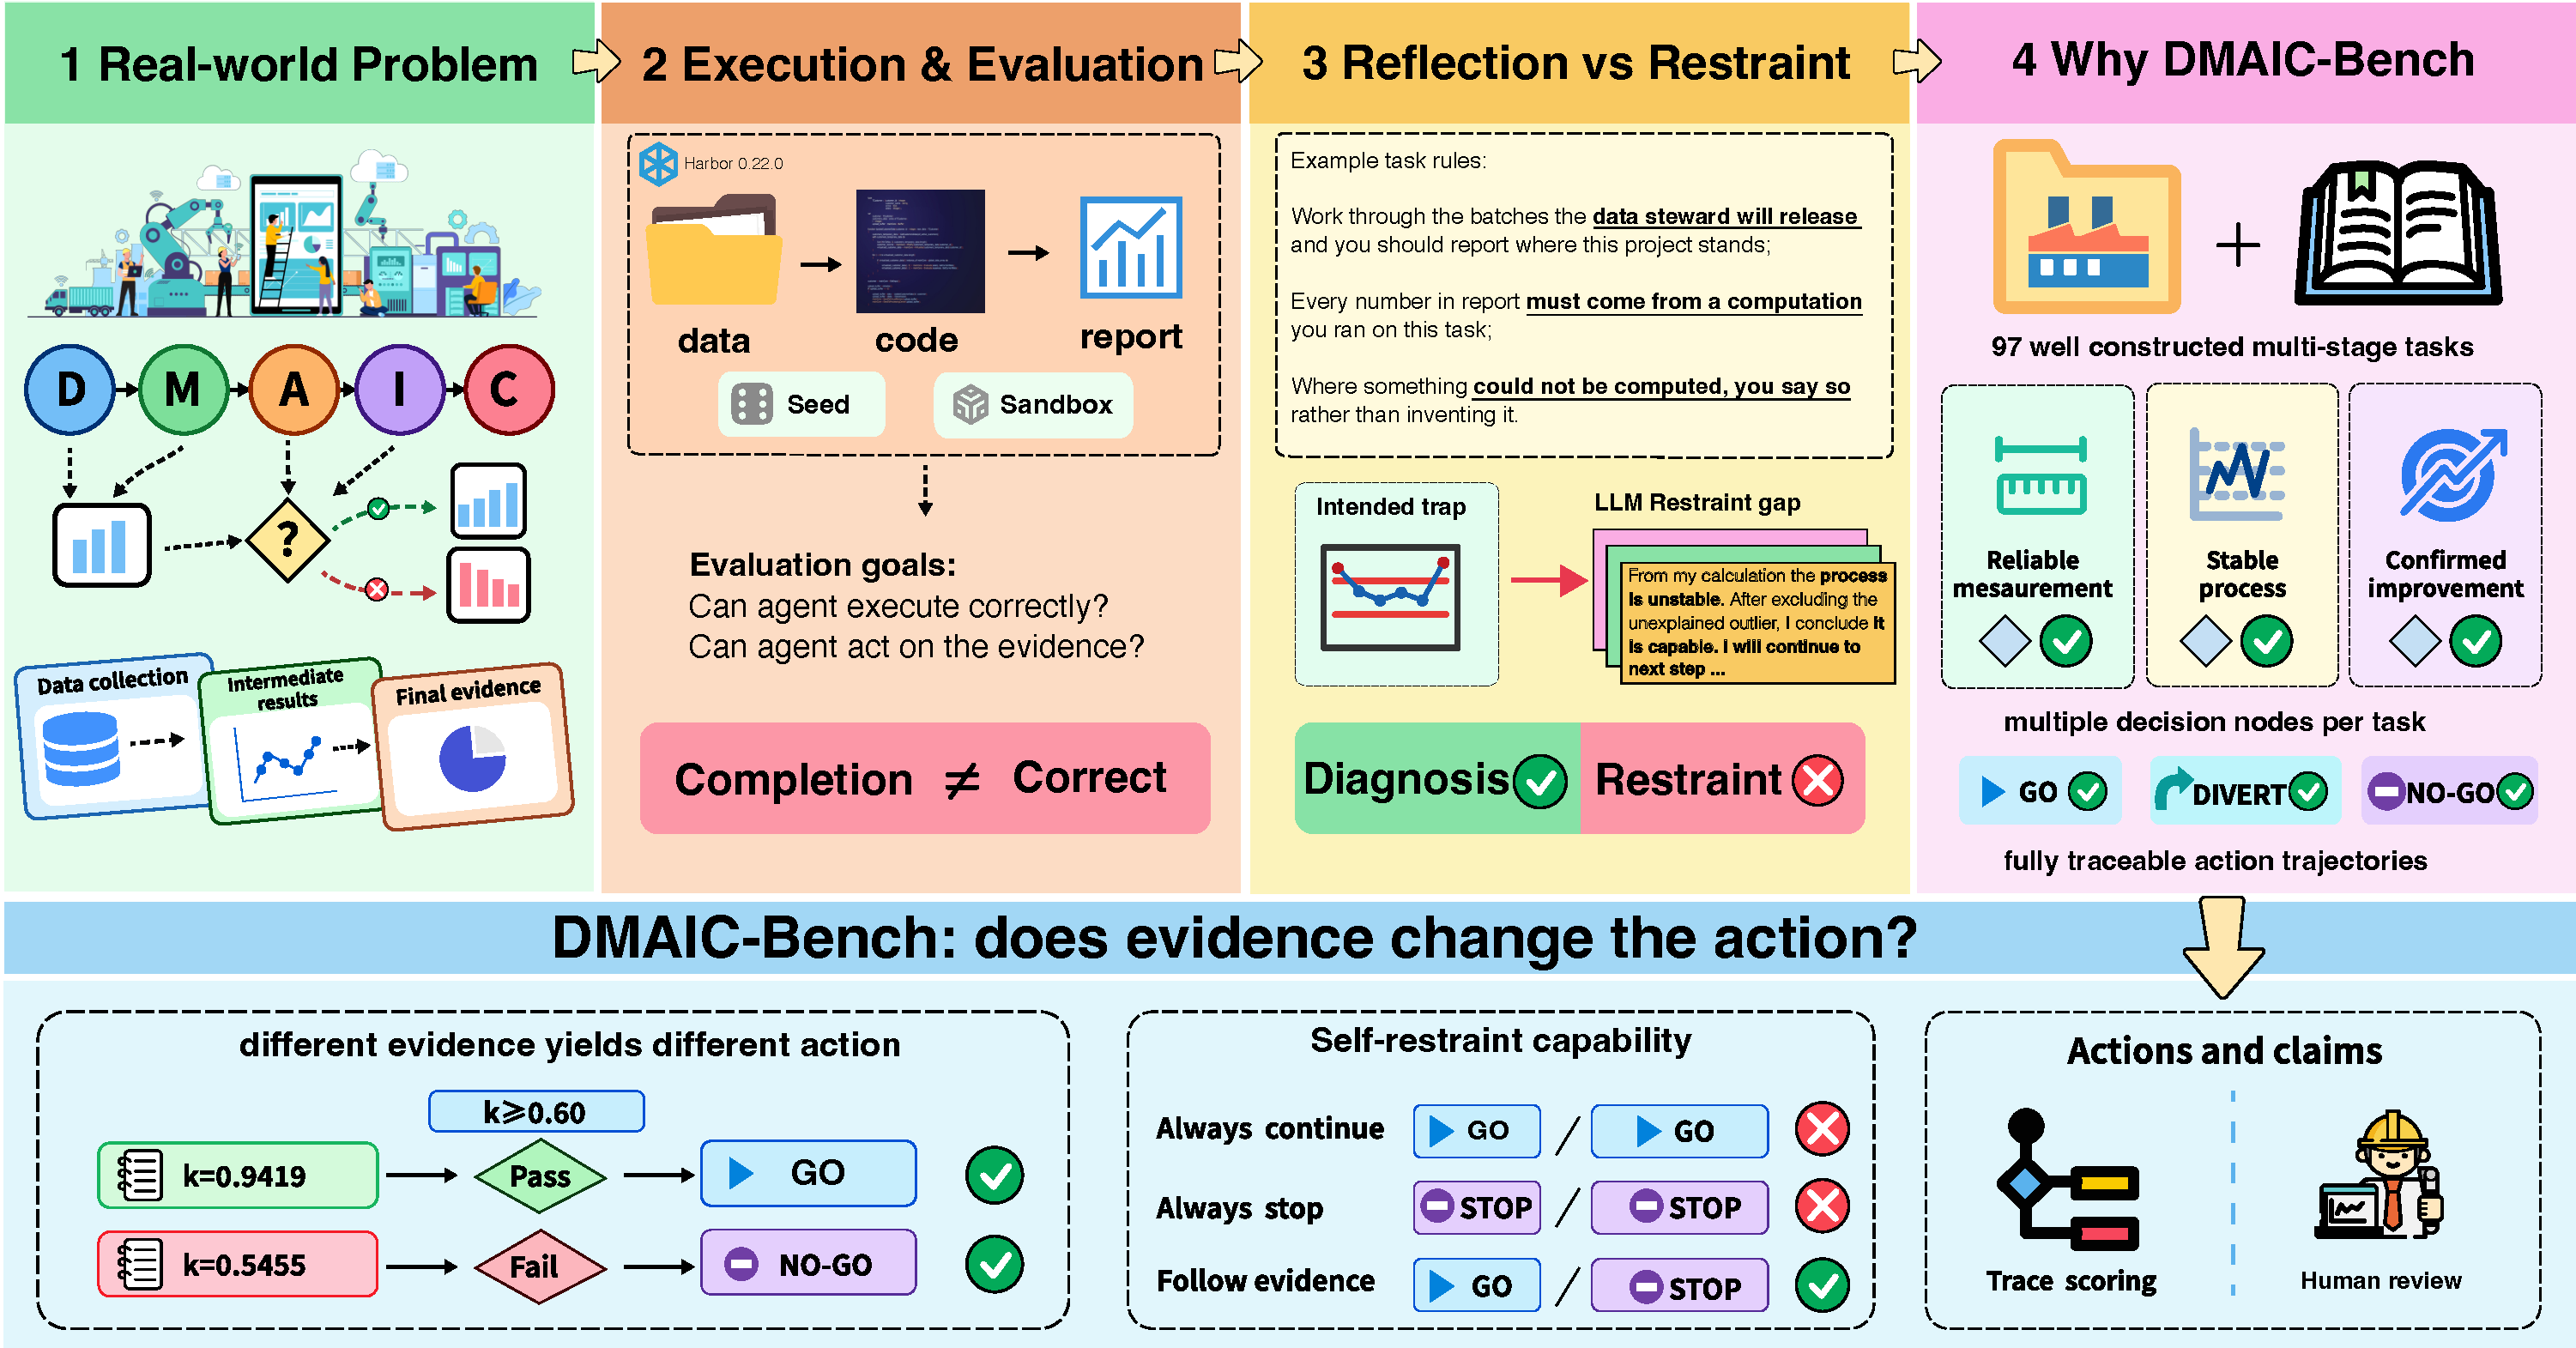
\includegraphics[width=0.94\linewidth]{figures/figure01_workflow.pdf}
\caption{\textbf{Overall illustration of DMAIC-Bench.} (1)~We start from evidence-dependent industrial workflows. (2)~We test execution and evidence-based decisions on seeded sandbox tasks. (3)~We distinguish correct diagnosis from warranted action. (4)~DMAIC standards and paired tasks evaluate self-restraint through trace scoring and human review.}
\label{fig:intro}
\end{figure}

This raises a question: \emph{can an agent in a multi-stage analytical task use computed evidence to choose correctly among continuing, diverting and stopping?} We call this capability \textbf{self-restraint}. Self-reflection asks an agent to critique its own output \citep{shinn2023reflexion,madaan2023selfrefine}; self-restraint asks whether computed evidence changes the next action; we test no reflection intervention.

Lean Six Sigma (DMAIC) and quality-engineering standards give explicit rules for this \citep{juran1999handbook,nist_handbook}. The Define--Measure--Analyze--Improve--Control cycle links stages through prerequisites \citep{montgomery2020isqc}: variance analysis requires gauge repeatability \citep{aiag2010msa}, capability indices require process stability \citep{aiagvda2026spc}, and interventions require empirical confirmation \citep{montgomery2013daoe}, so an untrusted gauge or an unstable process invalidates dependent analyses. The task does not say which prerequisite will fail; the agent must find out by intermediate analysis, and an evaluator can check whether proceeding, diverting or stopping is warranted at each of the case's graded forks.

\textbf{DMAIC-Bench} tests whether an agent governs its trajectory by computed evidence, stopping when prerequisites fail and proceeding when they hold. Each case is a guarded decision graph whose data steward checks declared prerequisites before releasing dependent batches. Of 66 graded forks, 40 have paired counterfactual variants, the same workflow position with seeded data that yield opposite diagnostic outcomes, so every no-go decision has a go counterpart and restraint is separated from blanket refusal. In total, 97 tasks span 15 industrial cases in four sectors, eight of them adapted from the closure reports of real black-belt improvement projects. The scorer reads the execution trace, so a forbidden computation counts as a route error even when the report withholds its result.

Across \nSystems{} models, execution-level matched-fork accuracy is \mGoRight\% for go decisions and \mStopRight\% for no-go decisions. Errors persist after correct diagnostics: \strictKnewW{} of \strictKnewN{} no-go decisions with reported and verified guard fields take the wrong route, and in \knewDiagFirst{} errors the diagnostic precedes the forbidden analysis. Independent expert review of a no-go sample from 11 agents finds reports acting on invalid evidence at \sTwoActed\% of reached no-go decisions. Explicit stopping permission improves some agents, but 12 of \nControls{} remain below 50\% no-go accuracy. We also validate the same framework on 16 RNA-seq and GWAS tasks in the life sciences, where the prerequisites differ. Our contributions are:
\begin{enumerate}
  \item \textbf{Benchmark Design:} DMAIC-Bench, 97 multi-step industrial tasks across 15 cases with runtime data-access guards and paired counterfactual instances that test warranted stopping against justified continuation.
  \item \textbf{Empirical Restraint Gap:} Evaluating \nSystems{} agents shows an execution-level gap, \mGoRight\% matched go accuracy versus \stopRightMin{}--\stopRightMax\% no-go accuracy, and in \knewDiagFirst{} errors agents report correct guard values before running analyses those diagnostics do not permit.
  \item \textbf{Expert Validation \& Intervention Limits:} Blinded expert review of a no-go sample from 11 agents finds reports acting on invalid evidence at \sTwoActed\% of reached no-go decisions. Instruction and runtime interventions improve some routing decisions, with effects that differ across agents and can reduce correct continuation.
\end{enumerate}

\section{Related work}
\label{sec:related}

We position DMAIC-Bench within three strands of research: agent and statistical benchmarks, self-reflection and abstention, and runtime enforcement and monitoring. Table~\ref{tab:related_benchmarks} compares DMAIC-Bench with existing benchmarks across seven design dimensions.

\begin{table}[!ht]
\caption{Comparison of benchmark design dimensions. \checkmark: dedicated component; $\times$: outside the benchmark's target; $\triangle$: related but indirect component; ---: not established by the cited description. For DMAIC-Bench the human column marks human-derived reference routes (eight cases follow black-belt closure reports) and expert confirmation of gate labels, not a measured human score.}
\label{tab:related_benchmarks}
\centering
\small
\setlength{\tabcolsep}{2.5pt}

\begin{tabular*}{\linewidth}{@{\extracolsep{\fill}}lccccccc@{}}
\toprule
{\fontsize{8}{9}\selectfont \thead{\textbf{Benchmark}}} & {\fontsize{8}{9}\selectfont \thead{\textbf{Dynamic}\\\textbf{route}}} & {\fontsize{8}{9}\selectfont \thead{\textbf{Runtime}\\\textbf{guards}}} & {\fontsize{8}{9}\selectfont \thead{\textbf{Sequential}\\\textbf{disclosure}}} & {\fontsize{8}{9}\selectfont \thead{\textbf{Valid}\\\textbf{stopping}}} & {\fontsize{8}{9}\selectfont \thead{\textbf{Tool}\\\textbf{execution}}} & {\fontsize{8}{9}\selectfont \thead{\textbf{Industrial}\\\textbf{topology}}} & {\fontsize{8}{9}\selectfont \thead{\textbf{Human}\\\textbf{baseline}}} \\
\midrule
SWE-bench \citep{jimenez2024swebench} & $\times$ & $\times$ & $\times$ & $\times$ & \checkmark & $\times$ & --- \\
MLE-bench \citep{chan2025mlebench} & $\times$ & $\times$ & $\times$ & $\times$ & \checkmark & $\times$ & \checkmark \\
Terminal-Bench \citep{merrill2026terminalbench} & $\times$ & $\times$ & $\times$ & $\times$ & \checkmark & $\times$ & --- \\
PaperBench \citep{starace2025paperbench} & $\times$ & $\times$ & $\times$ & $\times$ & \checkmark & $\times$ & \checkmark \\
$\tau$-bench \citep{yao2024taubench} & $\triangle$ & $\times$ & $\triangle$ & $\triangle$ & \checkmark & $\times$ & --- \\
StatQA \citep{zhu2024statqa} & $\times$ & $\times$ & $\times$ & $\times$ & $\times$ & $\times$ & \checkmark \\
P-Bench \citep{miao2026fisher} & $\times$ & $\times$ & $\times$ & $\times$ & \checkmark & $\times$ & --- \\
SDBench \citep{nori2025sdbench} & $\triangle$ & $\times$ & \checkmark & $\triangle$ & $\triangle$ & $\times$ & \checkmark \\
SOP-Bench \citep{nandi2026sopbench} & $\triangle$ & $\times$ & $\times$ & $\times$ & \checkmark & $\triangle$ & --- \\
AgentAbstain \citep{liu2026agentabstain} & $\times$ & $\times$ & $\triangle$ & \checkmark & \checkmark & $\times$ & --- \\
Agentic Abstention \citep{luo2026agenticabstention} & $\times$ & $\times$ & $\triangle$ & \checkmark & \checkmark & $\times$ & --- \\
\midrule
\textbf{DMAIC-Bench} & \checkmark & \checkmark & \checkmark & \checkmark & \checkmark & \checkmark & $\triangle$ \\
\bottomrule
\end{tabular*}
\end{table}

\paragraph{Agent and statistical benchmarks.}
SWE-bench, MLE-bench, PaperBench, and Terminal-Bench assess completed artifacts \citep{jimenez2024swebench,chan2025mlebench,starace2025paperbench,merrill2026terminalbench}; $\tau$-bench tests interactive tool use \citep{yao2024taubench,yao2025tau2bench}. In data analysis and statistics, StatQA, P-Bench, and StatEval probe analytical choices, inferential errors, and statistical reasoning \citep{zhu2024statqa,miao2026fisher,lu2025stateval}; DS-1000, InfiAgent, and DA-Code evaluate data-science code and data manipulation \citep{lai2023ds1000,hu2024infiagent,huang2024dacode}; and BLADE accommodates multiple defensible analytical paths \citep{gu2024blade}. Related suites target scientific discovery \citep{majumder2025discoverybench,chen2025scienceagentbench}, ML experimentation \citep{huang2024mlagentbench}, computational reproduction \citep{siegel2024corebench}, sequential clinical evidence disclosure \citep{nori2025sdbench}, and procedural adherence \citep{nandi2026sopbench,chen2026chibench}. None of these suites directly scores whether a computed diagnostic licenses the next analysis (Table~\ref{tab:related_benchmarks}). DMAIC-Bench evaluates that decision across multi-stage industrial projects and treats justified stopping as a valid terminal route whenever a prerequisite has failed. 

\paragraph{Self-reflection and abstention.}
Reflexion, Self-Refine, and CRITIC revise outputs through reflection or external feedback \citep{shinn2023reflexion,madaan2023selfrefine,gou2024critic}; self-correction, however, hinges on the quality of available feedback \citep{huang2024cannot,kamoi2024when}. Abstention predates agents: selective question answering declines when calibrated confidence is low \citep{kamath2020selective}, refusal-aware tuning teaches a model to say it does not know \citep{zhang2024rtuning}, and a survey sorts abstention by query, model and values \citep{wen2025knowyourlimits}. Agent abstention benchmarks examine abstention or escalation under ambiguity, missing information, conflicting objectives or prohibited operations \citep{liu2026agentabstain,trinh2026hilbench,huang2026conflictgui,asif2026blindspot}, and Agentic Abstention studies interaction-revealed prerequisites and stopping times \citep{luo2026agenticabstention}. AgentAbstain pairs tasks that differ in whether they can be answered; DMAIC-Bench pairs seeds at one workflow position, so only a computed value differs, and the matched instances isolate whether the agent's \emph{own correct diagnostic} governs the next action.

\paragraph{Runtime enforcement and monitoring.}
Shielding intercepts unsafe actions \citep{alshiekh2018shielding}, while guardrail systems constrain inputs, outputs, or tool calls \citep{rebedea2023nemo,inan2023llamaguard}. AI-control research studies monitoring under untrusted policies \citep{greenblatt2024control}. In DMAIC-Bench, the data steward enforces prerequisites before releasing dependent batches. External access controls cannot remove action bias: when a diagnostic and the analysis it forbids use the same released batch, the restraint decision rests with the agent. Section~\ref{sec:steward} and Appendix~\ref{app:steward} state which dependencies the environment enforces.




\section{The DMAIC-Bench framework}
\label{sec:bench}

\begin{figure}[H]
\centering
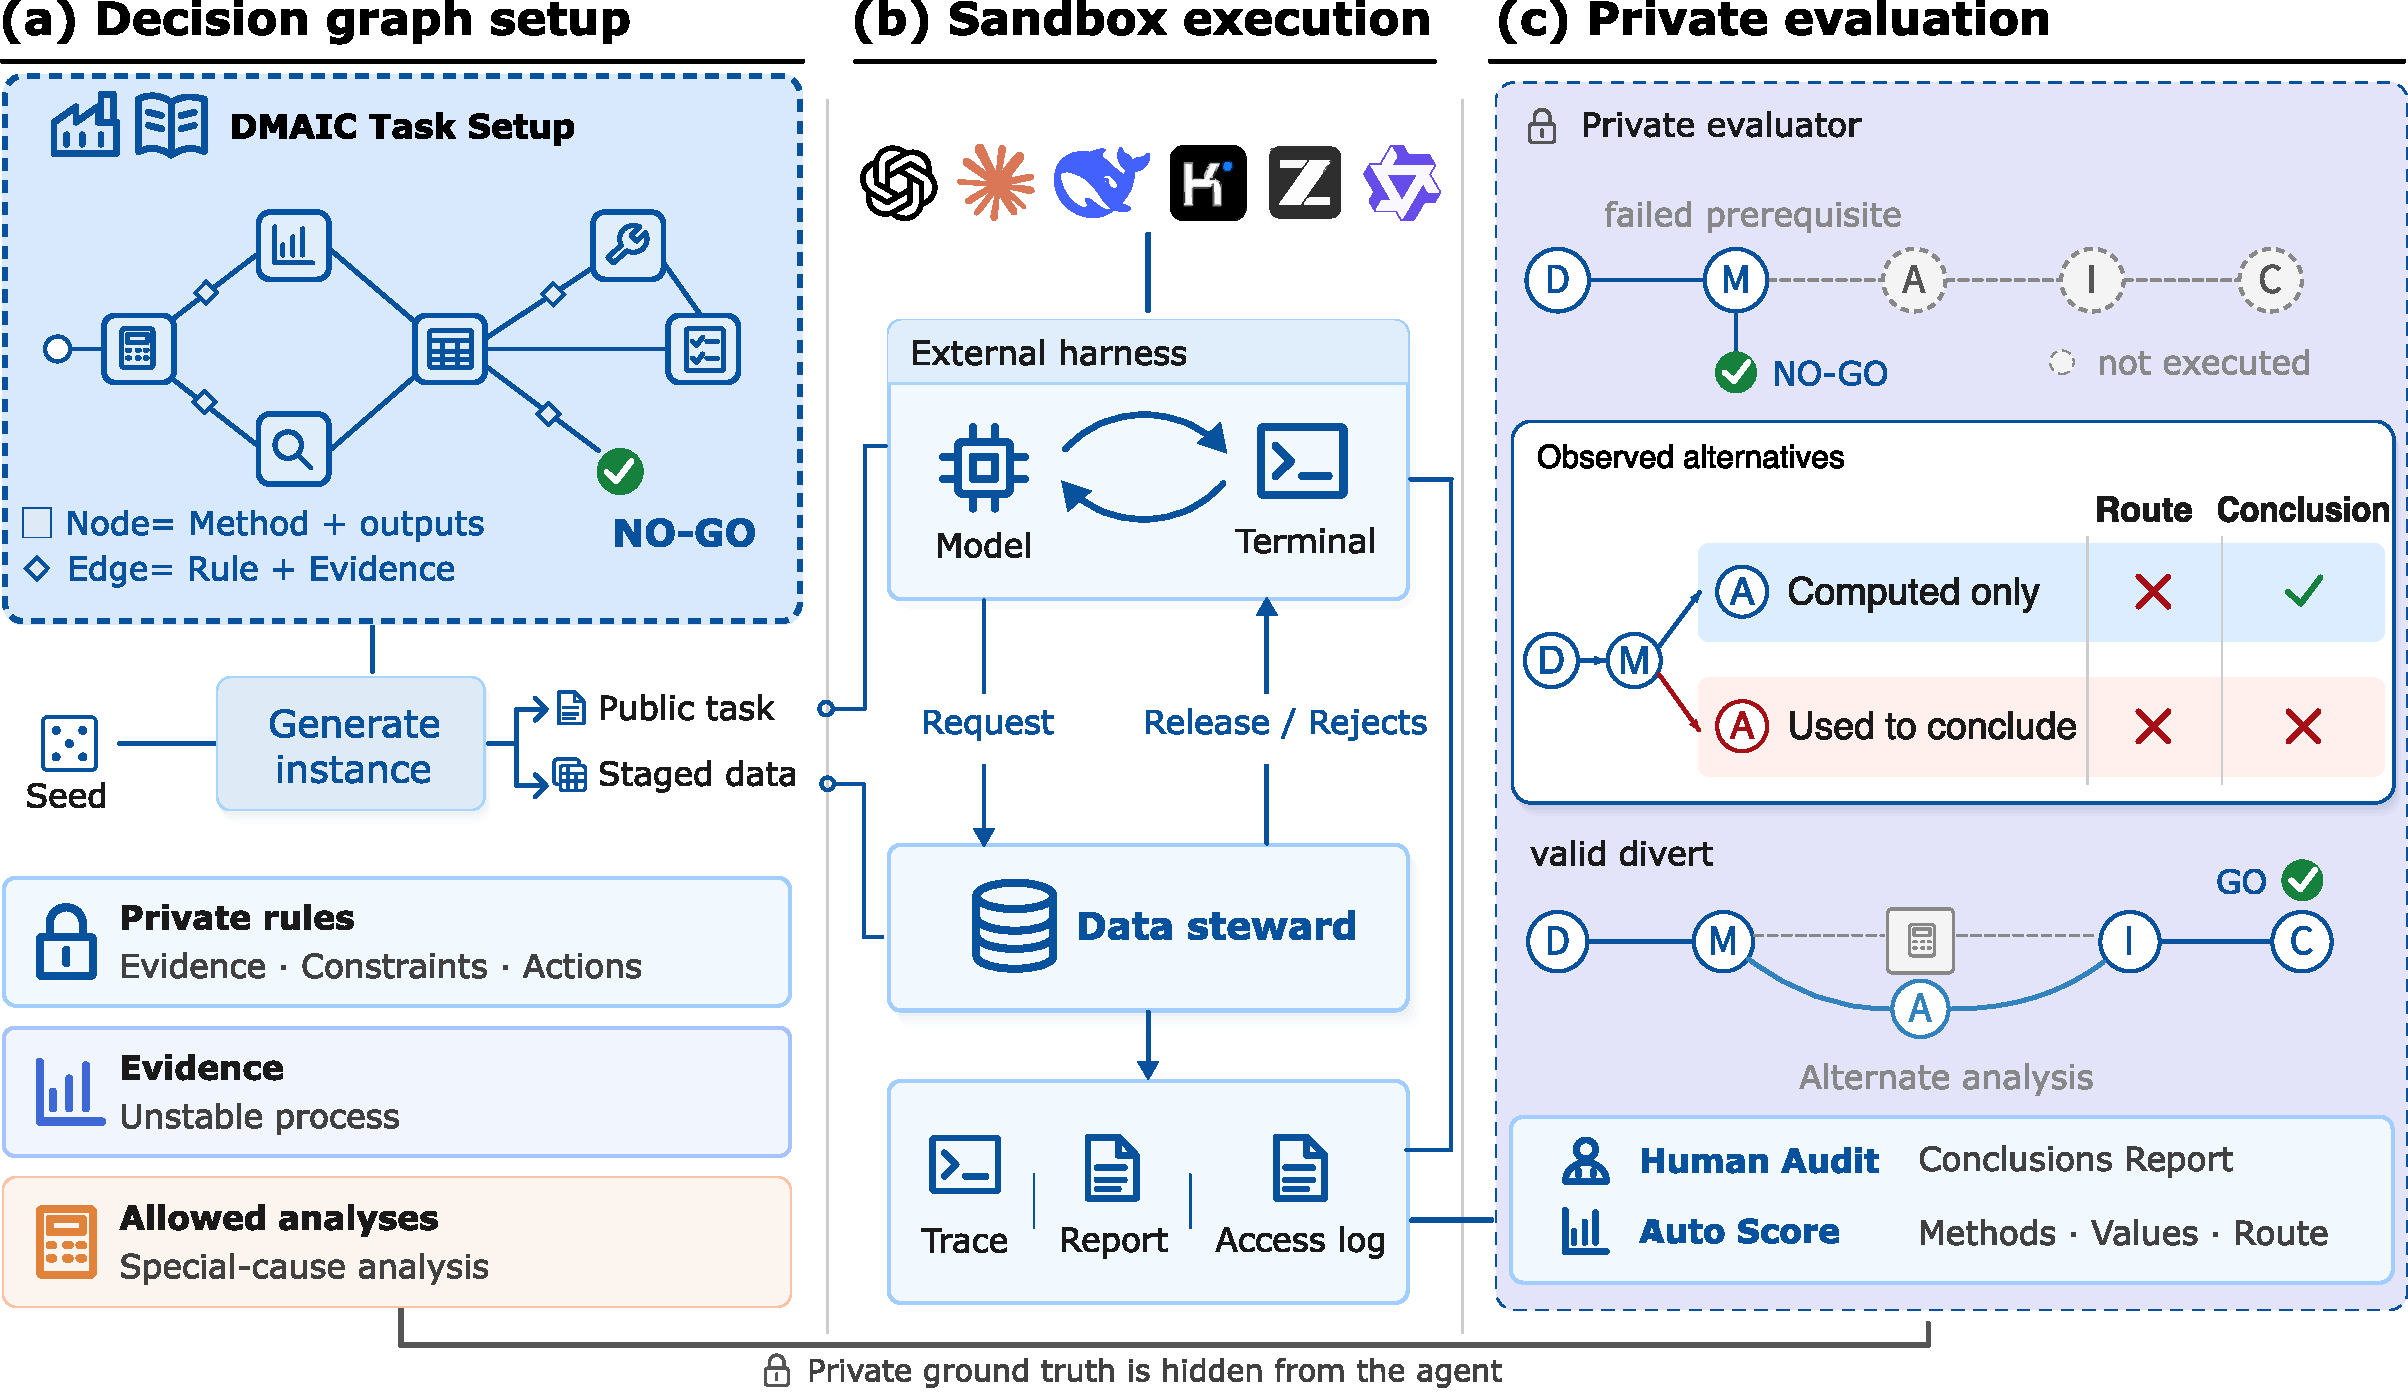
\includegraphics[width=0.94\linewidth]{figures/figure02_architecture.pdf}
\caption{\textbf{DMAIC-Bench architecture.}
\textbf{(a)} Guarded graphs generate seeded tasks and reference routes.
\textbf{(b)} A shared harness executes tool calls in a sandbox where a data steward enforces access prerequisites.
\textbf{(c)} Private scoring evaluates execution; expert review assesses final claims.}
\label{fig:arch}
\end{figure}

\noindent\textbf{Framework Overview and Task Formalization.}
Figure~\ref{fig:arch} illustrates the end-to-end lifecycle of DMAIC-Bench, which formalizes each benchmark instance as a seeded industrial project, $x = (\iota, G, s, \beta)$, comprising a natural-language business instruction $\iota$, a guarded decision graph $G$, a data seed $s$, and a finite query budget $\beta$ for shop-floor process facts. An agent interacts with the containerized environment to request data batches, execute statistical analyses, and dynamically govern its execution trajectory: proceeding (GO), rerouting (DIVERT), or terminating (NO-GO). The required deliverables are a structured execution trace $\tau$ and a narrative engineering report $\mathcal{R}$, where justified early termination upon a failed prerequisite constitutes a valid, successful route completion. Section~\ref{sec:tasks} covers task synthesis and guarded graphs (a), Section~\ref{sec:steward} the data steward (b), and Section~\ref{sec:scoring} scoring, expert review of final claims (c), and quality control.

\subsection{Benchmark Construction}
\label{sec:tasks}
\label{sec:tiers}

\begin{wrapfigure}{R}{0.4\textwidth}
\centering
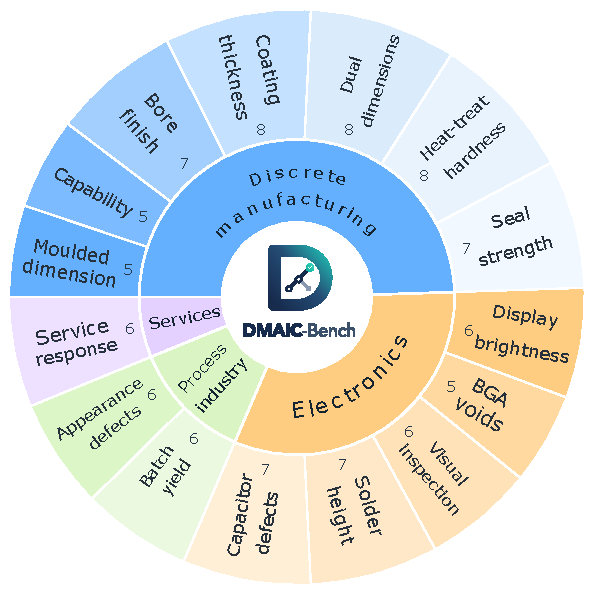
\includegraphics[width=\linewidth]{figures/figure03_task_breakdown.pdf}
\caption{\textbf{Task breakdown.} 97 tasks by industry (inner) and scenario (outer).}
\label{fig:corpus-overview}
\end{wrapfigure}

We construct cases from industrial problems, characteristics, units, specification limits and analytical stages. Eight retain routes from black-belt closure reports. Seven use routes derived from standards in project-informed scenarios. Appendix~\ref{app:corpus} documents the corpus in datasheet form \citep{gebru2021datasheets}; released tasks carry generated data and omit source prose and identifying details.

Each case is a guarded graph $G=(V,E,\Phi)$, with analytical stages and terminal actions in $V$, admissible transitions in $E$, and predicates on upstream diagnostics in $\Phi$. The gauge guard applies the AIAG MSA-4 acceptance criteria \citep{aiag2010msa}:
\begin{equation}
\phi_{\mathrm{go}}=(\mathrm{SV}_{\mathrm{gauge}}\leq0.30)\wedge(\mathrm{ndc}\geq5),
\end{equation}
where $\mathrm{SV}_{\mathrm{gauge}}$ is the gauge contribution to study variation and $\mathrm{ndc}$ is the number of distinct categories. A generator and seed determine data batches; computed diagnostics determine guard outcomes and the reference route. Counterfactual seeds reverse a prerequisite at the same workflow position, including branches absent from the source project. Of \nForks{} graded case--node forks, \nMatched{} contain both go and no-go seeds, providing a go counterpart for every no-go decision.

Figure~\ref{fig:corpus-overview} breaks down the corpus across its 15 cases, 97 tasks, and 175 nodes, spanning four sectors, five DMAIC phases, and 29 methods. Reference routes average 6.0 analyses and 3.1 graded decisions; prior analyses govern 284 of 300 decisions. As detailed in Table~\ref{tab:corpus}, the routes define \nTierA{} A-go, \nTierB{} B-divert, and \nTierC{} C-stop tasks; the latter two groups, \nStopTasks{} tasks, require diversion or stopping.

\subsection{Agent Interaction}
\label{sec:steward}

Agents interface with the benchmark via a shared harness, executing tools within isolated containers with pinned scientific-Python libraries and no network access. A local data steward exposes four core operations: requesting shop-floor data batches (\texttt{request}), declaring prerequisite verdicts (\texttt{declare}), querying domain process facts (\texttt{provision}), and inspecting available data inventory (\texttt{status}). Only \texttt{provision} queries consume the finite budget $\beta$. The steward logs declarations and verifies access prerequisites; it never reveals or checks against private ground truth, which resides in an isolated verifier container that the agent's execution environment cannot reach at any point of a run, and the steward's configuration contains no method identifiers.

Access controls govern cross-batch transitions: while 9 stop tasks place the GO branch behind explicit steward locks, 40 no-go tasks (including all B-divert instances) provide the data upfront and require restraint without environmental blocking. Each episode logs all released batches, declared verdicts, and query turns, terminating either upon the submission of the execution trace and final report or at the wall-clock limit. Appendices~\ref{app:taskdef}, \ref{app:steward}, and~\ref{app:roster} detail the interaction contract, the steward's operations, and the container execution parameters used across every run.


\subsection{Evaluation and Quality Control}
\label{sec:scoring}
\label{sec:qc}

\paragraph{Automated execution scoring.}
The private verifier scores execution traces against reference routes $\rho^*(x)$ and checks batch access against steward audit logs. Branch-level accuracy evaluates individual GO/NO-GO choices: a matched fork requires correct decisions across all paired seeds at that position, while task-level route success requires the full reference route. Aggregate reward combines routing accuracy with method adherence and numerical precision:
\begin{equation}
R = \mathcal{H}(R_m, P_m, F_n, A_r)\,(1-U)\,I,
\end{equation}
where $\mathcal{H}$ denotes the harmonic mean of method recall ($R_m$), method precision ($P_m$), numerical fidelity ($F_n$), and routing accuracy ($A_r$). Misuse $U \in [0, 1]$ penalizes violated statistical assumptions, while the binary integrity gate $I \in \{0, 1\}$ zeroes the reward if withheld data are accessed; without it a misspecified reward would leave that shortcut open \citep{pan2022rewardmisspecification}. Justified early stopping is credited on its valid prefix, whereas forbidden computation constitutes a route error whether or not the report endorses the result. Route accuracy thus measures execution restraint, not the validity of final claims; the two are distinct outcomes, which \S\ref{sec:study2} assesses separately by expert review.

\paragraph{Expert audit of report validity.}
Because an execution error does not imply that an agent endorsed the invalid result, we separately audit the narrative report $\mathcal{R}$. Certified Black-Belt experts independently evaluated blinded checkpoints across two distinct studies; Appendix~\ref{app:expert} reports their agreement as Fleiss' and Cohen's $\kappa$ \citep{fleiss1971agreement,cohen1960agreement}. Study 1 audited 30 checkpoints across all 15 cases (26 case--seed instances), informing scoring revisions such as admitting a declared Welch alternative for unequal variances. Study 2 evaluated 60 fresh checkpoints across 12 cases under a frozen protocol to assess report claims without further scorer tuning, distinguishing \emph{acting on invalid evidence} (asserting forbidden conclusions or recommending disqualified actions) from computing an invalid metric while withholding its conclusion. Neither study serves as an end-to-end task-solving baseline for human experts.

\paragraph{Benchmark consistency checks.}
Source checks trace numerical claims to original reports, recompute formulas, screen duplicate material, and distinguish observed from standards-derived routes. Graph, guard, generator, and numerical verifications, the checks recommended for agentic benchmarks \citep{zhu2025abc}, ensure that every reference solution scores 1.000 and the null agent scores 0.000. These scores show that scorer and reference solutions agree; they cannot exclude a rule misapplied in both generator and scorer, which the expert confirmation of gate labels (\S\ref{sec:study2}) covers. Appendices~\ref{app:construction-qc} and~\ref{app:expert} document review protocols, independent votes and open discrepancies.
\definecolor{gaincolor}{RGB}{20, 120, 50}    %
\definecolor{flatcolor}{RGB}{120, 120, 120}  %
\definecolor{dropcolor}{RGB}{180, 40, 40}    %
\definecolor{shadecol}{gray}{0.96}           %



\section{Experiments}
\label{sec:results}

\begin{table}[t]
\caption{\textbf{Main results across default (Plain) and permission-to-stop (+Permit) conditions.} Ranked by 3-attempt mean Plain reward. Accuracy and diagnostic columns reflect attempt~1. $\Delta$: percentage point difference. GO Right counts all 248 GO decisions; matched-fork rates and case-clustered intervals for the rates and the $\Delta$ columns are in Table~\ref{tab:matched-ci}. Stopped (verif.): correct stops among NO-GO decisions with a verified guard value.}
\label{tab:main_results}
\centering
\small
\setlength{\tabcolsep}{2.5pt}
\renewcommand{\arraystretch}{1.0}
\begin{tabular*}{\linewidth}{@{\extracolsep{\fill}} r l cc ccc ccc cc @{}}
\toprule
& & \multicolumn{2}{c}{\textbf{Mean Reward $\uparrow$}} & \multicolumn{3}{c}{\textbf{NO-GO Right $\uparrow$ (\%)}} & \multicolumn{3}{c}{\textbf{GO Right $\uparrow$ (\%)}} & \multicolumn{2}{c}{\textbf{Diagnostics}} \\
\cmidrule(lr){3-4} \cmidrule(lr){5-7} \cmidrule(lr){8-10} \cmidrule(lr){11-12}
\textbf{Rank} & \textbf{Agent} & 
Plain & \cellcolor{shadecol}+Permit & 
Plain & \cellcolor{shadecol}+Permit & $\Delta$ & 
Plain & \cellcolor{shadecol}+Permit & $\Delta$ & 
\thead{Stopped\\(verif.)} & \thead{B-div.\\(18)} \\
\midrule
--- & Reference solution$^\dagger$ & 1.000 & \cellcolor{shadecol}---   & 100\% & \cellcolor{shadecol}---   & ---   & 100\% & \cellcolor{shadecol}---   & ---   & ---  & 18/18 \\
\midrule
1  & \logo{openai} GPT-6-astra       & 0.662 & \cellcolor{shadecol}0.717 & 23\%  & \cellcolor{shadecol}\textbf{79\%} & \textcolor{gaincolor}{\textbf{+56}} & 82\%  & \cellcolor{shadecol}67\%  & \textcolor{dropcolor}{-15} & 9/31 & 1/18 \\
2  & \logo{openai} GPT-5.6-sol        & 0.649 & \cellcolor{shadecol}0.674 & 21\%  & \cellcolor{shadecol}38\%          & \textcolor{gaincolor}{+17}          & 81\%  & \cellcolor{shadecol}77\%  & \textcolor{dropcolor}{-4}  & 8/28 & 0/18 \\
3  & \logo{moonshot} Kimi-k3          & 0.603 & \cellcolor{shadecol}0.648 & 17\%  & \cellcolor{shadecol}27\%          & \textcolor{gaincolor}{+10}          & 82\%  & \cellcolor{shadecol}81\%  & \textcolor{dropcolor}{-1}  & 5/26 & 0/18 \\
4  & \logo{anthropic} Claude-Sonnet-5 & 0.599 & \cellcolor{shadecol}0.644 & 19\%  & \cellcolor{shadecol}25\%          & \textcolor{gaincolor}{+6}           & 82\%  & \cellcolor{shadecol}81\%  & \textcolor{dropcolor}{-1}  & 5/21 & 0/18 \\
5  & \logo{deepseek} DeepSeek-v4-flash& 0.599 & \cellcolor{shadecol}0.652 & 21\%  & \cellcolor{shadecol}42\%          & \textcolor{gaincolor}{+21}          & 79\%  & \cellcolor{shadecol}77\%  & \textcolor{dropcolor}{-2}  & 5/23 & 0/18 \\
6  & \logo{deepseek} DeepSeek-v4-pro  & 0.592 & \cellcolor{shadecol}0.575 & 23\%  & \cellcolor{shadecol}23\%          & \textcolor{flatcolor}{0}            & 79\%  & \cellcolor{shadecol}77\%  & \textcolor{dropcolor}{-2}  & 7/27 & 0/18 \\
7  & \logo{zhipu} GLM-5.3             & 0.582 & \cellcolor{shadecol}0.636 & 21\%  & \cellcolor{shadecol}29\%          & \textcolor{gaincolor}{+8}           & 82\%  & \cellcolor{shadecol}83\%  & \textcolor{gaincolor}{+1}  & 7/22 & 0/18 \\
8  & \logo{openai} GPT-5.6-luna      & 0.564 & \cellcolor{shadecol}0.595 & \textbf{25\%}  & \cellcolor{shadecol}27\%          & \textcolor{gaincolor}{+2}           & 70\%  & \cellcolor{shadecol}73\%  & \textcolor{gaincolor}{+3}  & 9/22 & 4/18 \\
9  & \logo{anthropic} Claude-Fable-5.1& 0.557 & \cellcolor{shadecol}0.654 & 17\%  & \cellcolor{shadecol}\textbf{44\%}          & \textcolor{gaincolor}{\textbf{+27}} & 81\%  & \cellcolor{shadecol}81\%  & \textcolor{flatcolor}{0}   & 5/15 & 0/18 \\
10 & \logo{zhipu} GLM-5.3-Flash       & 0.556 & \cellcolor{shadecol}0.576 & 17\%  & \cellcolor{shadecol}19\%          & \textcolor{gaincolor}{+2}           & 82\%  & \cellcolor{shadecol}81\%  & \textcolor{dropcolor}{-1}  & 3/16 & 0/18 \\
11 & \logo{anthropic} Claude-Opus-5   & 0.542 & \cellcolor{shadecol}0.634 & 17\%  & \cellcolor{shadecol}25\%          & \textcolor{gaincolor}{+8}           & 78\%  & \cellcolor{shadecol}83\%  & \textcolor{gaincolor}{+5}  & 5/17 & 0/18 \\
12 & \logo{alibaba} Qwen3.8-max      & 0.404 & \cellcolor{shadecol}0.488 & 13\%  & \cellcolor{shadecol}27\%          & \textcolor{gaincolor}{+14}          & 77\%  & \cellcolor{shadecol}80\%  & \textcolor{gaincolor}{+3}  & 1/13 & 0/18 \\
13 & \logo{alibaba} Qwen3.8-flash    & 0.379 & \cellcolor{shadecol}0.441 & 10\%  & \cellcolor{shadecol}17\%          & \textcolor{gaincolor}{+7}           & 77\%  & \cellcolor{shadecol}78\%  & \textcolor{gaincolor}{+1}  & 2/11 & 1/18 \\
\bottomrule
\end{tabular*}
\vspace{8pt}
\end{table}

\subsection{Evaluation Protocol and Metrics}
\label{sec:setup}

We evaluate \nSystems{} frontier model agents from \nVendorsWord{} providers across all 97 tasks using Harbor 0.22.0's stock Terminal-Bench execution loop \citep{merrill2026terminalbench} under a single tagged corpus build and scorer. To preserve evaluation neutrality across vendors, DMAIC-Bench provides no proprietary agent scaffolding or custom prompt adapters, a choice that fixed-harness suites also make \citep{liu2024agentbench,xie2024osworld}. Each model completes three independent attempts per task. Under the default \emph{Plain} instruction, agents conduct the analytical workflow and compile an engineering report, with no prompt saying that justified stopping counts as completion. Appendix~\ref{app:roster} lists the runtime configurations, context budgets and model identifiers; steward audit logs record no unauthorized access to withheld batches in any of the reported runs.

Each complete episode traverses 300 evaluated decisions: 52 NO-GO and 248 GO choices. Within these decisions, \nMatched{} matched forks pair all 52 NO-GO instances with 146 topologically identical GO counterparts, isolating the role of the seeded data while keeping workflow positions fixed. Beyond single-attempt metrics, multi-trial consistency is evaluated via pass@$k$, the fraction of tasks succeeding in at least one of $k$ attempts \citep{chen2021codex}, and $\text{pass}^k$, the fraction succeeding across all $k$ attempts \citep{yao2024taubench}. To account for dependency structures among seeds sharing the same case topology, all confidence intervals are computed via case-clustered bootstrap resampling \citep{field2007clusterbootstrap}, with its limits at these cluster counts stated in Appendix~\ref{app:ranking}.

\Needspace{5\baselineskip}
\subsection{Evidence-Dependent Control at Matched Forks}
\label{sec:restraint}
\label{sec:ranking}
\label{sec:main}

Table~\ref{tab:main_results} shows the asymmetry. At matched forks, agents take the warranted route on \mGoRight\% of GO decisions, with an interval from 86 to 97, but on only \mStopRight\% of NO-GO decisions, with an interval from 8 to 30, a 73-point gap with an interval from 59 to 87 (Table~\ref{tab:matched-ci}). The strict criterion counts computation, not decisions; Table~\ref{tab:study2rules} rescores the audited sample under expert criteria.

The failure is not a uniform forward bias. As reported in Table~\ref{tab:matched-results}, only 0--7 of the 40 matched forks are resolved correctly on both sides by any individual agent. While \nForkSame{} forks show a persistent bias toward continuation, the two confirmation forks show the reverse: after a confirmation succeeds, agents run the go-back analysis anyway on \confirmGoW{} of \confirmGoN{} GO decisions, an inadmissible branch (E3) rather than a stop, yet miss only \confirmStopW{} of \confirmStopN{} NO-GO decisions. At the same workflow position, the choice derails once the seeded data flip the warranted branch.

\begin{table}[!ht]
\caption{\textbf{Where self-restraint fails.} First-attempt phase accuracy and error shares (\%).}
\label{tab:decision-breakdown}
\centering
\begingroup
\fontsize{7.5}{9}\selectfont
\setlength{\tabcolsep}{1.2pt}
\renewcommand{\arraystretch}{1.06}
\newcommand{\bdcell}[3]{\cellcolor[HTML]{#1}\textcolor{#2}{#3}}
\newcommand{\bdhead}[2]{\begin{tabular}[c]{@{}c@{}}\textbf{#1}\\[-0.4pt]{\fontsize{6}{7}\selectfont\color{black!55}\textit{n}=#2}\end{tabular}}
\newcommand{\bderrhead}[1]{\begin{tabular}[c]{@{}c@{}}\textbf{#1}\\[-0.4pt]{\fontsize{6}{7}\selectfont\phantom{\textit{n}=00}}\end{tabular}}
\begin{tabular}{@{}>{\centering\arraybackslash}p{18pt}@{\hspace{4pt}}>{\raggedright\arraybackslash}p{80pt}@{\hspace{4pt}}*{4}{>{\centering\arraybackslash}p{\dimexpr(\linewidth-144.8pt)/15\relax}}@{\hspace{5pt}}*{6}{>{\centering\arraybackslash}p{\dimexpr(\linewidth-144.8pt)/15\relax}}@{\hspace{5pt}}*{5}{>{\centering\arraybackslash}p{\dimexpr(\linewidth-144.8pt)/15\relax}}@{}}
\toprule
 & & \multicolumn{4}{c}{\textcolor[HTML]{08519C}{\textbf{NO-GO accuracy (\%)}}} & \multicolumn{6}{c}{\textcolor[HTML]{08519C}{\textbf{GO accuracy (\%)}}} & \multicolumn{5}{c@{}}{\textcolor[HTML]{A50F15}{\textbf{Error share (\%)}}} \\
\cmidrule(lr){3-6}\cmidrule(lr){7-12}\cmidrule(l){13-17}
\textbf{Rank} & \textbf{Agent} & \bdhead{all}{52} & \bdhead{M}{35} & \bdhead{A}{12} & \bdhead{I}{5} & \bdhead{all}{248} & \bdhead{D}{6} & \bdhead{M}{129} & \bdhead{A}{94} & \bdhead{I}{7} & \bdhead{C}{12} & \bderrhead{E1} & \bderrhead{E2} & \bderrhead{E3} & \bderrhead{E4} & \bderrhead{E5} \\
\midrule
1 & \logo{openai.png}GPT-6-astra & \bdcell{8DB8D8}{black}{23} & \bdcell{74A9D1}{black}{17} & \bdcell{72A9D0}{black}{17} & \bdcell{C66C6F}{black}{80} & \bdcell{C26165}{black}{82} & \bdcell{DCAAAC}{black}{67} & \bdcell{AF2A30}{white}{94} & \bdcell{D79D9F}{black}{69} & \bdcell{D49496}{black}{71} & \bdcell{CE8285}{black}{75} & \bdcell{E8EEF3}{black}{46} & \bdcell{3685BE}{black}{1} & \bdcell{9EC2DD}{black}{27} & \bdcell{94BDDA}{black}{25} & \bdcell{3182BD}{black}{0} \\
2 & \logo{openai.png}GPT-5.6-sol & \bdcell{85B4D6}{black}{21} & \bdcell{69A3CD}{black}{14} & \bdcell{72A9D0}{black}{17} & \bdcell{C66C6F}{black}{80} & \bdcell{C5686C}{black}{81} & \bdcell{F7F6F6}{black}{50} & \bdcell{B02E33}{white}{93} & \bdcell{D9A2A5}{black}{68} & \bdcell{EBD5D6}{black}{57} & \bdcell{CE8285}{black}{75} & \bdcell{E7EDF2}{black}{46} & \bdcell{3182BD}{black}{0} & \bdcell{B7D1E4}{black}{34} & \bdcell{80B1D4}{black}{20} & \bdcell{3182BD}{black}{0} \\
3 & \logo{moonshot.png}Kimi-k3 & \bdcell{75AAD1}{black}{17} & \bdcell{5295C7}{black}{9} & \bdcell{72A9D0}{black}{17} & \bdcell{C66C6F}{black}{80} & \bdcell{C36367}{black}{82} & \bdcell{F7F6F6}{black}{50} & \bdcell{B02E33}{white}{93} & \bdcell{D79D9F}{black}{69} & \bdcell{D49496}{black}{71} & \bdcell{C05B5F}{black}{83} & \bdcell{F3F5F6}{black}{49} & \bdcell{3182BD}{black}{0} & \bdcell{D7E4EE}{black}{42} & \bdcell{5597C7}{black}{9} & \bdcell{3182BD}{black}{0} \\
4 & \logo{anthropic.png}Claude-Sonnet-5 & \bdcell{7DAFD3}{black}{19} & \bdcell{5E9DCA}{black}{11} & \bdcell{72A9D0}{black}{17} & \bdcell{C66C6F}{black}{80} & \bdcell{C26165}{black}{82} & \bdcell{F7F6F6}{black}{50} & \bdcell{B02E33}{white}{93} & \bdcell{D18B8E}{black}{73} & \bdcell{DAE6EF}{black}{43} & \bdcell{CE8285}{black}{75} & \bdcell{F3F5F6}{black}{49} & \bdcell{3182BD}{black}{0} & \bdcell{B2CEE3}{black}{33} & \bdcell{7AADD2}{black}{19} & \bdcell{3182BD}{black}{0} \\
5 & \logo{deepseek.png}DeepSeek-v4-flash & \bdcell{85B4D6}{black}{21} & \bdcell{5E9DCA}{black}{11} & \bdcell{94BDDA}{black}{25} & \bdcell{C66C6F}{black}{80} & \bdcell{C87175}{black}{79} & \bdcell{F7F6F6}{black}{50} & \bdcell{B64045}{white}{89} & \bdcell{D79D9F}{black}{69} & \bdcell{A2C5DE}{black}{29} & \bdcell{C05B5F}{black}{83} & \bdcell{DDE8EF}{black}{44} & \bdcell{3182BD}{black}{0} & \bdcell{BBD4E5}{black}{35} & \bdcell{85B4D6}{black}{21} & \bdcell{3182BD}{black}{0} \\
6 & \logo{deepseek.png}DeepSeek-v4-pro & \bdcell{8DB8D8}{black}{23} & \bdcell{69A3CD}{black}{14} & \bdcell{72A9D0}{black}{17} & \bdcell{A50F15}{white}{100} & \bdcell{C87175}{black}{79} & \bdcell{F7F6F6}{black}{50} & \bdcell{B53C41}{white}{90} & \bdcell{D79D9F}{black}{69} & \bdcell{A2C5DE}{black}{29} & \bdcell{CE8285}{black}{75} & \bdcell{D7E4EE}{black}{42} & \bdcell{3484BE}{black}{1} & \bdcell{B5D0E4}{black}{33} & \bdcell{8EB9D8}{black}{24} & \bdcell{3182BD}{black}{0} \\
7 & \logo{zhipu.png}GLM-5.3 & \bdcell{85B4D6}{black}{21} & \bdcell{5E9DCA}{black}{11} & \bdcell{94BDDA}{black}{25} & \bdcell{C66C6F}{black}{80} & \bdcell{C26165}{black}{82} & \bdcell{F7F6F6}{black}{50} & \bdcell{AF2A30}{white}{94} & \bdcell{D28E91}{black}{72} & \bdcell{EBD5D6}{black}{57} & \bdcell{DCAAAC}{black}{67} & \bdcell{F0F3F5}{black}{48} & \bdcell{3182BD}{black}{0} & \bdcell{D4E2ED}{black}{41} & \bdcell{5B9BC9}{black}{11} & \bdcell{3182BD}{black}{0} \\
8 & \logo{openai.png}GPT-5.6-luna & \bdcell{94BDDA}{black}{25} & \bdcell{96BEDB}{black}{26} & \bdcell{5295C7}{black}{8} & \bdcell{E7C9CA}{black}{60} & \bdcell{D6999C}{black}{70} & \bdcell{F7F6F6}{black}{50} & \bdcell{C36568}{black}{81} & \bdcell{E5C5C6}{black}{61} & \bdcell{3182BD}{black}{0} & \bdcell{CE8285}{black}{75} & \bdcell{ACCAE1}{black}{31} & \bdcell{3A88C0}{black}{3} & \bdcell{99BFDB}{black}{27} & \bdcell{CBDDEA}{black}{39} & \bdcell{3484BE}{black}{1} \\
9 & \logo{anthropic.png}Claude-Fable-5.1 & \bdcell{75AAD1}{black}{17} & \bdcell{5295C7}{black}{9} & \bdcell{72A9D0}{black}{17} & \bdcell{C66C6F}{black}{80} & \bdcell{C36568}{black}{81} & \bdcell{F7F6F6}{black}{50} & \bdcell{AF2A30}{white}{94} & \bdcell{D9A2A5}{black}{68} & \bdcell{D49496}{black}{71} & \bdcell{CE8285}{black}{75} & \bdcell{F0F3F5}{black}{48} & \bdcell{3182BD}{black}{0} & \bdcell{EBF0F4}{black}{47} & \bdcell{428CC2}{black}{4} & \bdcell{3182BD}{black}{0} \\
10 & \logo{zhipu.png}GLM-5.3-Flash & \bdcell{75AAD1}{black}{17} & \bdcell{478FC3}{black}{6} & \bdcell{72A9D0}{black}{17} & \bdcell{A50F15}{white}{100} & \bdcell{C36367}{black}{82} & \bdcell{F7F6F6}{black}{50} & \bdcell{B3353A}{white}{91} & \bdcell{D18B8E}{black}{73} & \bdcell{A2C5DE}{black}{29} & \bdcell{B3353A}{white}{92} & \bdcell{EEF2F4}{black}{48} & \bdcell{3484BE}{black}{1} & \bdcell{B8D2E5}{black}{34} & \bdcell{6FA7CF}{black}{16} & \bdcell{3484BE}{black}{1} \\
11 & \logo{anthropic.png}Claude-Opus-5 & \bdcell{75AAD1}{black}{17} & \bdcell{5295C7}{black}{9} & \bdcell{72A9D0}{black}{17} & \bdcell{C66C6F}{black}{80} & \bdcell{C87376}{black}{78} & \bdcell{F7F6F6}{black}{50} & \bdcell{B3353A}{white}{91} & \bdcell{DEB1B3}{black}{65} & \bdcell{D49496}{black}{71} & \bdcell{E9D0D1}{black}{58} & \bdcell{E0EAF0}{black}{44} & \bdcell{3182BD}{black}{0} & \bdcell{F5F6F6}{black}{49} & \bdcell{4890C4}{black}{6} & \bdcell{3182BD}{black}{0} \\
12 & \logo{alibaba.png}Qwen3.8-max & \bdcell{66A1CC}{black}{13} & \bdcell{478FC3}{black}{6} & \bdcell{5295C7}{black}{8} & \bdcell{C66C6F}{black}{80} & \bdcell{CA777A}{black}{77} & \bdcell{F7F6F6}{black}{50} & \bdcell{B4393E}{white}{91} & \bdcell{DEB1B3}{black}{65} & \bdcell{DAE6EF}{black}{43} & \bdcell{DCAAAC}{black}{67} & \bdcell{E2EBF1}{black}{45} & \bdcell{3182BD}{black}{0} & \bdcell{EEDEDF}{black}{55} & \bdcell{3182BD}{black}{0} & \bdcell{3182BD}{black}{0} \\
13 & \logo{alibaba.png}Qwen3.8-flash & \bdcell{5698C8}{black}{10} & \bdcell{3C88C0}{black}{3} & \bdcell{3182BD}{black}{0} & \bdcell{C66C6F}{black}{80} & \bdcell{CA797C}{black}{77} & \bdcell{F7F6F6}{black}{50} & \bdcell{B4393E}{white}{91} & \bdcell{DDADAF}{black}{66} & \bdcell{DAE6EF}{black}{43} & \bdcell{F7F6F6}{black}{50} & \bdcell{E4ECF1}{black}{45} & \bdcell{3182BD}{black}{0} & \bdcell{EFE0E1}{black}{55} & \bdcell{3182BD}{black}{0} & \bdcell{3182BD}{black}{0} \\
\midrule
\textemdash & \emph{Expert labels (blind)} & \bdcell{A91A20}{white}{98} & \bdcell{AB2127}{white}{96} & \bdcell{A50F15}{white}{100} & \bdcell{A50F15}{white}{100} & \bdcell{C66C6F}{black}{80} & \bdcell{F4F4F4}{gray}{\textemdash} & \bdcell{C05B5F}{black}{83} & \bdcell{C66C6F}{black}{80} & \bdcell{DCAAAC}{black}{67} & \bdcell{F4F4F4}{gray}{\textemdash} & \bdcell{F4F4F4}{gray}{\textemdash} & \bdcell{F4F4F4}{gray}{\textemdash} & \bdcell{F4F4F4}{gray}{\textemdash} & \bdcell{F4F4F4}{gray}{\textemdash} & \bdcell{F4F4F4}{gray}{\textemdash} \\
\bottomrule
\end{tabular}
\par\vspace{3pt}
\begin{minipage}{\linewidth}
\fontsize{6.7}{8}\selectfont\raggedright
\textbf{E1}: continued past a failed no-go precondition; \textbf{E2/E4}: no-go/go fork unreached (diagnostic unrun).\\
\textbf{E3}: took an inadmissible go branch; \textbf{E5}: stopped where the route continues.\\
\textit{n}: decisions per model; experts: agreement with benchmark labels on \bdExpertNogoN{} no-go and \bdExpertGoN{} go forks, not a task-solving baseline; \textemdash: not evaluated.
\par\vspace{2pt}
\setlength{\fboxsep}{1.5pt} Correct (\%): \colorbox[HTML]{3182BD}{\makebox[13pt]{\textcolor{black}{0}}}\colorbox[HTML]{F7F6F6}{\makebox[13pt]{\textcolor{black}{50}}}\colorbox[HTML]{A50F15}{\makebox[13pt]{\textcolor{white}{100}}}\hfill Share of errors (\%): \colorbox[HTML]{3182BD}{\makebox[13pt]{\textcolor{black}{0}}}\colorbox[HTML]{F7F6F6}{\makebox[13pt]{\textcolor{black}{50}}}\colorbox[HTML]{A50F15}{\makebox[13pt]{\textcolor{white}{100}}}
\end{minipage}
\endgroup

\end{table}

Figure~\ref{fig:results-summary}A shows that NO-GO accuracy stays within a narrow band of \stopRightMin{}--\stopRightMax\% across all models, despite overall rewards spanning 0.379 to 0.662. Table~\ref{tab:decision-breakdown} shows that the deficit spans both Measure and Analyze phases. Appendix~\ref{app:ranking} confirms that alternative reward aggregations leave these branch verdicts unchanged and reports case-clustered intervals, since few-run point estimates can hide substantial uncertainty in rankings \citep{agarwal2021precipice}.



\Needspace{7\baselineskip}
\paragraph{Repeated-attempt reliability.}
\label{sec:reliability}
Figure~\ref{fig:results-summary}B compares sporadic success with multi-run consistency across 97 tasks. 13-agent pass@3 reaches 23--37\% while strict three-run reproducibility ($\text{pass}^3$) drops to 10--29\% (Appendix~\ref{app:reliability}). Single-run metrics therefore mask frequent routing mistakes. On adaptive B-divert tasks, $\text{pass}^3$ is zero for \pkBdivZeroCount{} of \nSystems{} agents and tops out at only \pkBdivThreeMax{} (2/18 tasks), so models rarely reproduce adaptive rerouting across independent attempts at the same seeded task.


\subsection{From Correct Diagnostics to Invalid Actions}
\label{sec:diagnostics_to_actions}

High method recall (\recallMin{}--\recallMax{}) shows that agents can execute the required analytical steps. Of the \stopW{} NO-GO errors, \strictKnewW{} follow guard values that the agent reported and the verifier confirmed, \wrongValW{} follow a wrong value, \unverW{} an unverifiable one, \unobsW{} an unreported one, \disagreeW{} a value that implied the other branch, and \noneW{} no computation at all. In \knewDiagFirst{} of the \strictKnewW{}, the failing diagnostic appears in the trace before the forbidden analysis. The restraint finding proper is this verified subset, where \strictKnewStopped{} of \strictKnewN{} decisions stop correctly; the other classes are computation or reporting failures (Appendix~\ref{app:decision-outcomes}).

Forbidden downstream computation (Type~E1 error) accounts for \bdContinuedShare\% of all NO-GO errors, whereas only \bdNogoUnreached{} decisions never reach the fork. On adaptive B-divert tasks, across \bdivN{} first attempts on \nTierB{} instances, only \bdivRight{} complete the legitimate rerouted path; \bdivCap{} continue to compute process capability indices ($C_p/C_{pk}$) after control-chart diagnostics invalidate statistical stability prerequisites \citep[ISQC 8e, \S8.3]{montgomery2020isqc}. Appendix~\ref{app:decision-outcomes} confirms that the errors are continuation decisions at reached forks, not early timeouts that never reach the fork.

\begin{figure}[!t]
\centering
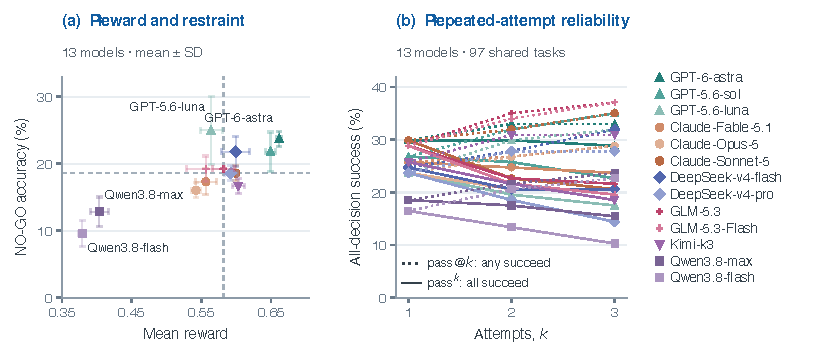
\includegraphics[width=\linewidth]{figures/figure04_results_summary.pdf}
\caption{\textbf{Reward, restraint, and reliability.} \textbf{(a)} Across-attempt means and SDs; median reference lines. \textbf{(b)} Dotted lines show success on any of the first $k$ attempts, solid lines on all $k$.}
\label{fig:results-summary}

\end{figure}



\subsection{From Execution Errors to Report Validity}
\label{sec:study2}

Execution traces reveal invalid computations, but agents might withhold flawed diagnostics from their final deliverables. Study~2 therefore conducted blinded expert audits on \sTwoN{} fresh task units under the frozen protocol of Section~\ref{sec:qc}. This audit sample, drawn from 12 cases and the 11 agents whose campaigns were complete when the study was frozen (the two Qwen agents finished later), comprises \sTwoStopN{} NO-GO decisions (stratified by mechanism and scorer verdict, reweighted to the population) and \sTwoGoN{} unweighted matched GO counterparts. Experts confirmed the benchmark's gate labels on \sTwoGateStop/\sTwoStopN{} NO-GO and \sTwoGateGo/\sTwoGoN{} GO units; Appendix~\ref{app:expert} lists the five disagreements, none of which changed a label. Among \sTwoIncN{} sampled NO-GO route failures, \sTwoIncActedK{} reports asserted forbidden conclusions or recommended disqualified actions, and \sTwoIncAcceptK{} withheld the invalid metric or adopted an alternative the reviewers accepted as a valid substitute.

In Figure~\ref{fig:study2}A, across the population-weighted NO-GO sample, narrative reports act on invalid evidence at \sTwoActed\% of reached NO-GO decisions, with an interval from 31\% to 61\%, while GO-side over-claiming reaches \sTwoGoActed\%. On these audited units, NO-GO route accuracy is \sTwoRouteStopRight\% against an expert semantic accuracy of \sTwoSemStop\%, with GO values of \sTwoRouteGoRight\% and \sTwoSemGo\%: a gap of 73 percentage points under execution-level route scoring but 25 points under expert semantic assessment. Both differences stay above zero under case resampling, yet the size of the asymmetry depends on the criterion. Table~\ref{tab:study2rules} in Appendix~\ref{app:expert} rescores the sample under each criterion, and Appendix~\ref{app:propagation} traces how invalid intermediate results propagate into final conclusions. Three LLM readers as judges \citep{zheng2023judging,zhuge2024agentjudge} agree with the experts only moderately and disagree with one another on the no-go rate, so we report the expert estimates (Table~\ref{tab:llmreader}).



\subsection{Instruction and Runtime Interventions}
\label{sec:control}

To test whether models fail to stop only because of prompt-induced completion pressure, we evaluate the \emph{permit-stop} instruction across all 97 tasks. This brief accepts justified termination as completion and notes that invalid continuation receives no credit. Table~\ref{tab:main_results} shows the trade-off: GPT-6-astra improves its NO-GO accuracy from \ctlMaxRightFrom\% to \ctlMaxRightTo\%, but its GO accuracy simultaneously degrades from \ctlGPTastraPlainGoRight\% to \ctlGPTastraPermitGoRight\%. DeepSeek-v4-pro remains stalled at \ctlMinRightTo\% NO-GO accuracy, and 12 of \nControls{} evaluated agents still fail to break 50\%, so completion bias alone cannot explain the failure of self-restraint at forks with failed prerequisites, whatever the instruction says about completion.

A pre-registered replication on 32 paired tasks contrasts this divergence across five conditions and 960 trials. Every condition runs the same tasks on a byte-identical truth package with three attempts per task, so the conditions differ only in the brief and, for one of them, a runtime channel; the two agents are the largest and the smallest movers in Table~\ref{tab:main_results}. Figure~\ref{fig:instruction-controls}B--C shows that permission lifts Astra from 2.3 to 10.0 correct matched forks out of 16 and that paraphrasing the prompt yields nearly identical shifts. DeepSeek is largely invariant to permission phrasing: the permission and its paraphrase leave it at \repDeepSeekvproPermitStopRight\% and \repDeepSeekvproParaphraseStopRight\% NO-GO accuracy, averaging under two correct paired forks of 16 under permission and under five under the paraphrase. 

A \emph{normative} prompt states the prerequisite rules without completion framing and raises DeepSeek to \repDeepSeekvproNormativeStopRight\% NO-GO accuracy, a gain of 25 points whose interval runs from 11 to 42, with GO accuracy essentially unchanged. Runtime warnings against declared predicates under the \emph{remind} condition add five points more, an increment whose interval from $-8$ to 17 includes zero, so the benefit of reminders beyond a stated rule is uncertain. For Astra the rule costs 42 points of GO accuracy, an interval from 65 to 14, and its 12-point NO-GO gain includes zero; reminders fall short of explicit permission. Permission rescues some stopping choices at the cost of warranted progress; a stated rule helps one model at no such cost and costs the other more than permission did. Appendix~\ref{app:ctlrep} documents the conditions, task counts and contrasts.

\begin{figure}[!t]
\centering
\captionsetup{justification=raggedright,singlelinecheck=false,skip=4pt}
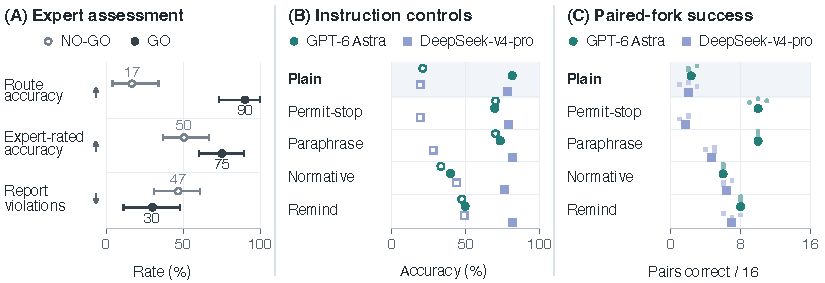
\includegraphics[width=\linewidth]{figures/figure05_expert_controls.pdf}
\caption{\textbf{Expert validation and instruction controls.} \textbf{(A)} Expert assessment; bars: case-clustered 95\% CIs. \textbf{(B)} GO (filled) and NO-GO (open) accuracy. \textbf{(C)} Matched forks correct on both sides, out of 16; large markers show three-attempt means, small markers individual attempts.}
\label{fig:expert-controls}
\label{fig:study2}
\label{fig:instruction-controls}
\end{figure}

\subsection{Cross-Domain Evaluation in the Life Sciences}
\label{sec:cross-domain}

To test transfer beyond industrial workflows, we extend DMAIC-Bench to sixteen seeded tasks in bulk RNA-seq and case-control GWAS. Domain methods and guard predicates follow genomic standards, with batch-confounding checks before differential expression \citep{leek2010tackling,love2014deseq2} and population-structure controls before association testing \citep{price2006principal}, while the interaction contract, data steward, and private verifier remain identical and every reference solution scores 1.000. Evaluating GPT-6-astra, GPT-5.6-sol, and GPT-5.6-luna across protocol and thresholds-only briefs shows that the framework transfers and, for the three agents tested, the residual errors take the same form: protocol-brief NO-GO accuracy is far higher than on the industrial tasks (Table~\ref{tab:cross-domain}a), yet 9 of the 10 errors follow a correctly computed diagnostic that warrants stopping (Appendix~\ref{app:portability}). Table~\ref{tab:cross-domain}b shows that omitting consequence framing drops NO-GO accuracy from 20/24 to 17/24, driven by the GWAS structure fork, which collapses from 4/6 to 0/6, while RNA-seq decisions remain unaffected. These runs do not show that the industrial rates generalise: brief, locks, domain and fork position vary together, and stating a rule's consequence changes the outcome. Appendix~\ref{app:portability} gives implementations and counts.

\begin{table}[H]
\caption{\textbf{Cross-domain evaluation.} Correct/graded decisions in RNA-seq and GWAS.}
\label{tab:cross-domain}
\centering
\small
\setlength{\tabcolsep}{2pt}
\begin{minipage}[t]{0.51\linewidth}
\textbf{(a) Protocol: three attempts}\par\smallskip
\begin{tabular*}{\linewidth}{@{\extracolsep{\fill}}lrrr@{}}
\toprule
\textbf{Agent} & \textbf{NO-GO} & \textbf{DIVERT} & \textbf{GO} \\
\midrule
\logo{openai.png}GPT-6-astra & 22/24 & 12/12 & 102/102 \\
\logo{openai.png}GPT-5.6-sol & 23/24 & 11/12 & 96/102 \\
\logo{openai.png}GPT-5.6-luna & 17/24 & 6/12 & 90/102 \\
\bottomrule
\end{tabular*}
\end{minipage}\hfill
\begin{minipage}[t]{0.46\linewidth}
\textbf{(b) NO-GO: first attempt}\par\smallskip
\begin{tabular*}{\linewidth}{@{\extracolsep{\fill}}lrr@{}}
\toprule
\textbf{Domain} & \textbf{Protocol} & \textbf{Thresholds} \\
\midrule
RNA-seq & 12/12 & 12/12 \\
GWAS & 8/12 & 5/12 \\
GWAS structure & 4/6 & 0/6 \\
\bottomrule
\end{tabular*}
\end{minipage}
\end{table}




\section{Conclusion}
\label{sec:conclusion}

DMAIC-Bench evaluates self-restraint, the capacity of agents to govern multi-stage analytical trajectories using computed evidence. Across 97 industrial tasks with paired counterfactual branches, frontier models reach \mGoRight\% on valid continuation routes but only \stopRightMin{}--\stopRightMax\% execution-level accuracy on decisions requiring justified stopping or diversion. In \knewDiagFirst{} instances, agents ran the forbidden computation after logging the failing diagnostic, and blinded expert audits of a NO-GO sample from 11 agents find reports acting on invalid evidence at \sTwoActed\% of reached no-go decisions. Stopping permission rescues some models at the cost of warranted progress, a stated rule helps one model and costs another, and reminders add little beyond the rule. The genomics extension shows that the framework transfers and that the remaining errors take the same form for the three agents tested, while failure rates depend on how prerequisites and consequences are stated. The paired design gives future work a test: an intervention that raises NO-GO accuracy has to hold GO accuracy at the same forks, and the stated rule passed that test for one agent and failed it for the other. The scorer, the audit records and the scripts that regenerate every number are released. Instilling self-restraint without paralysis is an open challenge for agents in high-stakes science and engineering.


\clearpage
\section*{AI use statement}
Generative AI tools assisted with this work in the following ways. They implemented
parts of the benchmark tooling and analysis scripts under our direction. They took part
in the design and implementation of the two life-sciences pilot cases, including the
seeded data generators and reference implementations; we specified this work, reviewed it
and validated it against the published sources cited in Appendix~\ref{app:portability}.
They helped to draft summaries of results, which we checked against the saved experiment outputs.
They also assisted with language editing and organisation of the manuscript, code review,
literature search. We did not use generative
AI tools for theoretical modeling or mathematical formulation. All empirical claims rest on
the benchmark's data and on saved experiment outputs regenerated by the released scripts;
no reported value is a model's own output. We are responsible for all final content.

\section*{Ethics statement}
Every published task is generated from a seed. The benchmark contains no source-project measurements, tables, figures or sentences, and identifies no source product, organisation or person. The private corpus of closure reports is not redistributed. No personal data is collected or
processed. The expert reviews assessed anonymised agent trajectories, not people, under
procedural blinding on a shared filesystem; no human-subject study was conducted and no
task was solved by a human for scoring. The benchmark evaluates whether an agent lets a
computed precondition constrain its conclusion; it is not a certification of statistical
competence, and a score on it should not be used to justify removing qualified human
review from industrial decisions. The tasks involve no safety-critical intervention: every
action is a computation on generated data inside a container.

\section*{Reproducibility statement}
The public repository ({\urlstyle{same}\url{https://github.com/psptpx/DMAIC-Bench-public}}) contains the case generators, the decision graphs and their
guards, the truth-package builder, the data steward, the scorer, and the analysis scripts
that regenerate every table and number in this paper from retained run artifacts
(\nolinkurl{scripts/restraint_analysis.py}, \nolinkurl{scripts/rescore.py}). A build check verifies that the same case and seed produce a byte-identical corpus. Every task scores 1.000 for a reference solution and 0.000 for a null agent. Campaigns ran in Harbor 0.22.0
with its stock agent loop and pinned scientific-Python libraries (Appendix~\ref{app:roster});
the scorer version and corpus build used for every reported number are tagged in the
repository, and the per-trial artifacts (trace, report, steward log, terminal recording,
scorecards) are distributed as an archive with the tagged release. The held-out split, its
selection rule and seed, and both blind-review packages with the human experts' records are released for independent inspection and reproduction of the review analyses.

\clearpage
\bibliographystyle{iclr2027_conference}
\bibliography{references}

\clearpage
\appendix
\addtocontents{toc}{\protect\setcounter{tocdepth}{2}}
\renewcommand{\contentsname}{Contents of Appendix}
{\setlength{\parskip}{0pt}\tableofcontents}
\clearpage
\raggedbottom
\setlength{\parskip}{4pt plus 1pt minus 1pt}
\setlength{\floatsep}{6pt plus 1pt minus 1pt}
\setlength{\textfloatsep}{6pt plus 1pt minus 1pt}
\setlength{\intextsep}{6pt plus 1pt minus 1pt}
\widowpenalty=10000
\clubpenalty=10000
\floatsetup[table]{capposition=top}
\captionsetup[table]{position=top,skip=6pt,font=normalsize}
\makeatletter
\setlength{\@fptop}{0pt}
\setlength{\@fpsep}{12pt}
\setlength{\@fpbot}{0pt plus 1fil}
\makeatother
\renewcommand{\topfraction}{0.9}
\renewcommand{\bottomfraction}{0.8}
\renewcommand{\textfraction}{0.08}
\renewcommand{\floatpagefraction}{0.75}

\section{Task definition}
\label{app:taskdef}

A task instance is a tuple $x = (\iota, G, s, \beta)$: a natural-language instruction
$\iota$ that names no statistical method (Appendix~\ref{app:instruction}); a case graph
$G = (V, E, \Phi)$ (\S\ref{sec:bench}); a seed $s \in \mathcal{S}$; and a
provision budget $\beta$. The seed generates the case's data batches
$\mathcal{B}_s = \{b_1, \dots, b_m\}$; every
truth value is recomputed from those batches by the reference verifiers at build time, so a
new seed changes data and truth together, and the correct route is
$\rho^*(x) = \operatorname{walk}(G, \mathbf{y}(s))$: the walk selected by the guards in $\Phi$ after evaluating the diagnostic outputs from those batches. The build derives each answer from the generated data. Workflow routing~\citep{vanderaalst2003workflow} and action
preconditions in planning~\citep{valmeekam2023planbench} provide related abstractions;
here the preconditions are statistical diagnostics computed during execution. Paired
seeds test whether a changed diagnostic reverses the action, a directional behavioral
test in the sense of CheckList~\citep{ribeiro2020checklist}.

Execution is an episode against the data steward (Appendix~\ref{app:steward}). Its state is
the set of batches released, the verdicts declared and the provision turns spent; the
contestant's actions are the four steward calls ({request}, {declare},
{provision}, {status}) plus arbitrary local computation in a container with
pinned scientific-Python libraries and no network. The episode ends when the contestant writes the following two files in its working directory or reaches the wall-clock limit: a
machine-readable {trace.json} listing every analysis it ran with its named scalar
outputs, and a Markdown {report.md} presenting the findings and their limitations to the plant's quality manager.

The evaluator scores the \emph{trace} and cross-checks it against the steward's audit log. It compares the implied route with $\rho^*$ (\textbf{pq}), the executed analyses with those required by the route (\textbf{ms\_recall}, \textbf{ms\_precision}), and reported values with recomputed truths (\textbf{nf}). It also checks whether the agent used data that the steward denied (\textbf{gate}). These components are combined as in \S\ref{sec:scoring}; a terminal world state or answer string is not the scoring target. Only the honesty axis reads the report, and that axis is released but excluded from reward (Appendix~\ref{app:limitations}). The score reflects the computations and their timing, even when the report describes the correct course of action (Appendix~\ref{app:example}).

\paragraph{What counts as a forbidden computation.}
The route is inferred from behaviour. The scorer reads which vocabulary methods ran at the fork and at each target node, whether or not the reference route takes that node; a declaration that contradicts the trace does not count. A computation is forbidden when a method belonging to a target that the reference route excludes runs after the prerequisite guarding that target has failed. Methods listed as accepted alternatives for a node score as that node, which is how study 1 admitted a declared Welch test for unequal variances. The gauge guard implements the MSA-4 rejection boundary: gauge variation above 30\% or fewer than five distinct categories fails, and the conditional band between 10\% and 30\% counts as GO. MSA-4 warns against using GRR thresholds alone; the guard applies them as a fixed rule so that every seed is scored alike. Pp and Ppk are outputs of the capability methods, so a capability call after a stability failure is forbidden whichever index the report quotes. Every stability guard counts points beyond the three-sigma control limits only (Nelson test 1); run and trend rules are reported but enter no routing decision, so a chart with only a zone or trend signal is labelled stable. Steps outside the 50-method vocabulary are not route evidence. The scorer does not read the report, so a report that computes a forbidden index and then withholds it keeps its route error; whether the report acted on the index is the question the expert review answers (\S\ref{sec:study2}).

\section{Corpus datasheet}
\label{app:corpus}

Table~\ref{tab:corpus} uses $|V|$ for graph nodes, ``guards'' for guarded edges and ``tasks'' for seeds, with one task per seed. A/B/C count tasks by routing tier (\S\ref{sec:tiers}); $\beta$ is the provision budget in turns. The source field distinguishes routes encoded from published standards (S) from those retaining a completed practitioner project's route (P; \S\ref{sec:unit}). Response type $y$ is continuous, attribute or mixed.

\begin{table}[!htbp]
\caption{The fifteen cases: graph size, generated tasks, routing tiers, provision budgets and provenance. Column definitions and source conventions are given in the text.}
\label{tab:corpus}
\centering
\footnotesize
\setlength{\tabcolsep}{2.5pt}
\begin{tabular}{@{}llllrrrlrl@{}}
\toprule
Case & Scenario & Industry & $y$ & $|V|$ & Guards & Tasks & A/B/C & $\beta$ & Src \\
\midrule
25 & moulded fitting dimension        & discrete    & cont. & 12 & 4 & 5 & 3/1/1 & 24 & S \\
26 & service-desk response commitment & services    & prop. & 12 & 5 & 6 & 3/1/2 & 24 & S \\
27 & batch yield on a process line    & process     & cont. & 14 & 5 & 6 & 4/1/1 & 24 & S \\
28 & display brightness uniformity    & electronics & cont. & 11 & 4 & 6 & 3/1/2 & 20 & S \\
29 & one critical characteristic      & discrete    & cont. &  5 & 1 & 5 & 4/1/0 & 16 & S \\
30 & bore surface finish, honing      & discrete    & cont. & 11 & 4 & 7 & 3/1/3 & 22 & S \\
31 & BGA solder void fraction         & electronics & cont. & 11 & 4 & 5 & 1/1/3 & 22 & S \\
32 & appearance defects vs.\ committed rate & process & prop. & 13 & 6 & 6 & 4/1/1 & 22 & P \\
33 & visual judgement repaired and re-proved & electronics & prop. & 11 & 4 & 6 & 4/1/1 & 26 & P \\
34 & coating thickness in its range   & discrete    & cont. & 14 & 6 & 8 & 5/2/1 & 24 & P \\
35 & two characteristics, the worse decides & discrete & cont. & 13 & 5 & 8 & 4/3/1 & 28 & P \\
36 & a screened change and its confirmation & electronics & cont. & 12 & 5 & 7 & 3/1/3 & 26 & P \\
37 & hardness: which comparison data admits & discrete & cont. & 14 & 6 & 8 & 3/1/4 & 26 & P \\
38 & real reduction, commitment still unmet & electronics & mixed & 10 & 5 & 7 & 2/1/4 & 26 & P \\
39 & response surface, optimum, confirmation & discrete & cont. & 12 & 6 & 7 & 2/1/4 & 28 & P \\
\midrule
Total & & & & 175 & 70 & 97 & \nTierA/\nTierB/\nTierC & & \\
\bottomrule
\end{tabular}

\end{table}

\textbf{Distribution.} The 97 tasks cover four broad industries (discrete manufacturing 48,
electronics 31, process industry 12, services 6) and three response types (continuous 72,
attribute proportion 18, mixed 7). The 175 nodes carry 70 guarded edges at \nForks{} graded
forks; \nMatched{} of those forks have both no-go and go seeds (\S\ref{sec:restraint}).
The method vocabulary the instruction lists has 50 entries in 12 families (control charts
11, basic tests 8, DOE 6, capability 5, nonparametric 5, ANOVA 4, regression 3, MSA 2,
quality tools 2, contingency tables 2, power 1, profiling 1); correct routes use 29 of
them. DOE, response-surface optimization and confirmation follow standard experimental design methods for estimating effects and checking proposed improvements~\citep{montgomery2013daoe}.

\textbf{Held-out split.} Five cases (cases 25, 26, 28, 34, 39; 32 tasks) form a reserved split to address case reuse and overfitting in agent evaluation~\citep{kapoor2024agentsmatter}. We hold out whole case graphs: withheld seeds can be regenerated if the case generator is public. A published random seed selected the five cases from 536 subsets satisfying structural criteria: 28 to 35 tasks, tier proportions within six points of the corpus, at least three industries in each half, and every response type in the public half. Contestant scores played no part in selection. Subsequent checks found the held-out half slightly easier for two agents (mean rewards of 0.575 vs.\ 0.549 and 0.685 vs.\ 0.622). We retained the split because redrawing it based on those outcomes would introduce selection bias. Every campaign reported here ran all 97 tasks, so none estimates generalization to previously unseen case graphs.

\textbf{Source routes and synthetic routes.} Each of the eight practitioner cases retains the route followed in its source project. Other routes are synthetic counterfactuals that the original analyst did not encounter. Source routes: case 32, the level
missed and a machine comparison; case 33, first study fails, rewritten criteria hold; case
34, one characteristic capable and one with its mean outside the limit ($C_{pk}<0$); case
35, one of two characteristics binds; case 36, a screened change with its confirmation (the
failed confirmation is synthetic); case 37, a candidate cause that is not a driver; case 38,
a reduction achieved with the commitment still missed; case 39, a fitted surface whose
optimum was confirmed (the non-fitting surface and the failed confirmation are synthetic).
The seven S cases use routes encoded from standards. Their scenarios may still draw on real projects, as the honing and BGA cases do; scenario provenance and the source of a route are recorded separately.

\textbf{Provenance.} Dataset documentation should distinguish origin, construction and
intended use~\citep{gebru2021datasheets}. No source data, table, figure or sentence is redistributed. The eight practitioner cases retain the scenario (industry, characteristic, units, limits), the judgments the analysts faced, and the order of magnitude of the values governing those decisions. Seeds generate every batch, and the generated data determine every truth value. Cases omit company, place and person names. The build requires public-identity mode to enforce this restriction in every released task package.

\section{Construction checks and review coverage}
\label{app:construction-qc}

The source survey records recovery of tables, grouped figures and legacy presentations,
OCR of image-only material, duplicate checks, source verification of quoted numbers and
recomputation of formulas. The records cover source preparation, including an earlier corpus, and do not certify the final 97 tasks individually. Private source
reports are not redistributed. The public artifacts document scenario and route provenance in \nolinkurl{docs/CASE_SOURCES.md} while withholding source identities and recording the origins of scenarios and decision structures separately.

\begin{table}[!htbp]
\caption{Distinct scopes of construction and validation evidence. A checkpoint review does not certify every branch of its case or every seed of its generator.}
\label{tab:construction-qc}
\centering\small
\begin{tabular}{@{}P{0.21\linewidth}P{0.32\linewidth}P{0.41\linewidth}@{}}
\toprule
Check & Coverage and evidence & Interpretation \\
\midrule
Source preparation & Extraction and source-survey records & Checks source interpretation; not instance-level acceptance. \\
Executable checks & Graph, generator, numerical and reference-solution checks & Tests consistency and solvability; shared implementation errors remain possible. \\
Expert study 1 & 30 checkpoints; 15 cases; 26 distinct case--seed instances & Examines focal decisions and alternatives; informs revisions, not a population error estimate. \\
Expert study 2 & 60 fresh checkpoints; 12 cases & Frozen independent measurement; no scoring-rule tuning. \\
\bottomrule
\end{tabular}

\end{table}

Study 1 includes one sampled no-go checkpoint per case, additional go checkpoints and six
purpose-selected boundary units. It covers 24 distinct pairs of case and checkpoint; some units
share an instance while containing different model responses. The original independent
votes and coordinator recomputations are retained. The resulting corrections include
restricting evidence to the relevant stage and admitting a declared Welch
alternative for unequal variances~\citep{welch1947generalization};
the case-37 implementation records the expert feedback for unit B022. The timing correction changed \nCrossStage{} of \nCrossStagePoints{} verdicts, although restricted description remains a scorer limitation. Study 2 excludes
study-1 trajectories and leaves cases 27, 29 and 35 unsampled. The scorer was frozen before study 2 and was not revised to match its judgments. The independent review therefore retains disagreements with the frozen scorer instead of treating them as labels for further tuning.

The release includes \nolinkurl{scripts/construction_qc_inventory.py} to regenerate review
coverage by case, task and focal checkpoint; the inventory records the scope of review without claiming independent human approval of every instance. The construction-QC record (\nolinkurl{docs/CONSTRUCTION_QC.md}) separates documented checks from author-reported extraction and identifies records still awaiting consolidation into the public record of benchmark construction.

\section{The task package and the steward protocol}
\label{app:steward}

\textbf{Lockable preconditions.} Table~\ref{tab:locks} classifies every
graded no-go fork by the precondition its guard reads. The steward can enforce a guard only if the guard has a public form the contestant can declare
against (a gate in the steward's vocabulary: {msa\_pass}, {msa\_ndc},
{stability\_pass}, {normality\_pass}, {screening\_significant}), and
the analysis it would forbid reads a \emph{different} batch from the one the guard is
computed on, so that withholding that batch is possible. \lkNoGateTypes{} of the eight
precondition types have no public form (attribute agreement, capability against a target,
confirmation), and most stability guards use the same process run as the capability calculation they constrain. Of \lkForks{} no-go forks \lkCross{} are cross-batch and \lkLocked{}
are locked. The contestant must enforce the remaining prerequisites itself. Table~\ref{tab:locks} records which decisions require this restraint because the required data are already available and access controls cannot block the downstream computation.

\begin{table}[!htbp]
\caption{No-go forks and decisions across 97 tasks, grouped by precondition type. Columns distinguish public steward gates, cross-batch dependencies and locks in the shipped configuration. A fork whose guard reads two precondition types appears in both rows, so the totals are row sums; the distinct counts are the 40 matched no-go forks and 52 no-go decisions per episode of \S\ref{sec:results}.}
\label{tab:locks}
\centering
\footnotesize
\begin{tabular}{@{}lrrlrr@{}}
\toprule
\thead{Precondition} & \multicolumn{1}{c}{\thead{No-go\\forks}} & \multicolumn{1}{c}{\thead{No-go\\decisions}} & \thead{Public\\gate} & \multicolumn{1}{c}{\thead{Cross-batch\\forks}} & \multicolumn{1}{c}{\thead{Locked\\forks}} \\
\midrule
gauge study (\%SV, \%tol) & 8 & 13 & yes & 8 & 6 \\
distinct categories (ndc) & 5 & 9 & yes & 5 & 3 \\
attribute agreement ($\kappa$) & 3 & 4 & no & 3 & 0 \\
statistical control & 16 & 18 & yes & 3 & 1 \\
normality & 5 & 6 & yes & 5 & 0 \\
screening significance & 5 & 7 & yes & 4 & 2 \\
capability against target & 2 & 3 & no & 2 & 1 \\
confirmation / fit & 2 & 2 & no & 1 & 0 \\
\midrule
Total & 46 & 62 & & 31 & 13 \\
\bottomrule
\end{tabular}


\end{table}

\textbf{Contestant access.} The container holds the rendered
instruction, a steward service on loopback with its command-line client, and the
steward's configuration: the batch labels and topics it routes on, the prerequisite locks,
and the budget. Task data enter the filesystem only after a successful {request}, which writes the released batch as JSON to a per-task directory. The truth package (the
graph, the truths with tolerances, the fork targets, the probe's method) lives in
the verifier's container and is never mounted into the agent's. The steward's configuration contains no method identifiers. The contestant selects analyses from the task context and the evidence in each released batch.

\begin{table}[!htbp]
\caption{The steward's four actions.}
\label{tab:steward-actions}
\centering
\footnotesize
\begin{tabular}{@{}lP{0.29\linewidth}P{0.42\linewidth}l@{}}
\toprule
Action & Argument & Effect & Billed \\
\midrule
\texttt{request}   & plain-language description of the batch wanted & routed onto one batch by its topics; on success the batch is written to disk and a preview returned & no \\
\texttt{declare}   & public criterion name, value & records the verdict the contestant claims (e.g.\ \texttt{msa\_pass true}); the steward does not check it against the truth & no \\
\texttt{provision} & one question to the process owner & answers a process fact from a fixed fact list & one turn \\
\texttt{status}    & --- & batches still available, turns spent & no \\
\bottomrule
\end{tabular}

\end{table}

Each JSON reply reports the outcome, refusal code, gate, stage and provision budget through {outcome}, {refusal}, {gate}, {stage\_id}, {turns\_used} and {max\_turns}.

\begin{table}[!htbp]
\caption{Steward refusal codes. Replies identify the outcome, gate or stage, and remaining budget.}
\label{tab:refusals}
\centering
\footnotesize
\begin{tabular}{@{}lP{0.78\linewidth}@{}}
\toprule
Refusal & Meaning \\
\midrule
\texttt{locked}     & a prerequisite batch has not been requested yet, or a public criterion the batch waits on has not been declared; the reply names the criterion, its threshold and the handbook it comes from \\
\texttt{denied}     & the batch (or, in a probe, one field of it) has been checked and does not exist; the instruction says to state the gap, not to invent it \\
\texttt{unroutable} & the description matched no batch; ask again in other words \\
\texttt{exhausted}  & the provision budget is spent \\
\texttt{invalid}    & a \texttt{declare} whose key is not a public criterion \\
\texttt{firewall}   & a \texttt{provision} that asks the process owner for a method or an acceptance threshold rather than a process fact \\
\bottomrule
\end{tabular}

\end{table}

\textbf{Lock implementation.} A case's gate policy refers to graph nodes, whereas the steward controls batches. Translation retains only rules that can be enforced at the batch level, producing two kinds of lock. An \emph{order lock}
releases a batch only after a named earlier batch has been requested. A \emph{verdict
lock} additionally waits for a {declare} of a public criterion: gauge acceptance
(\%StudyVariation $\le 30$; distinct categories $\ge 5$), stability, screening significance
or normality, each with its handbook citation in the refusal message. A guard is
translated into a verdict lock only when it is cross-batch and has such a public form; a
guard whose value is computed \emph{from} the batch it would gate (stability before a
capability index on the same process run; normality before the choice of test) cannot be
enforced by construction, and the attribute-agreement criterion has no public form. Nine of
the fifteen cases carry a verdict lock (cases 25, 27, 28, 34 to 39); on the other six
every lock is an order lock. Read at the no-go decision itself (the last fork on the
correct route whose guard fails), nine of the \nTierC{} C-no-go tasks have the go
branch behind a verdict lock (cases 25 s4, 27 s4, 28 s4 to 5, 34 s4, 35 s4, 37 s5, 38 s4, 39 s4); the other 22 C-no-go tasks and all \nTierB{} B-divert tasks have no verdict lock on that branch and require the contestant to enforce the precondition itself. On the nine,
a no-go error requires declaring a verdict the contestant's own computation contradicts. The four tasks of \S\ref{sec:steward} deliberately omit a lock on a guard with a public form. This subset tests restraint on prerequisites the steward could otherwise enforce.

\textbf{Honesty probes.} Twelve tasks ship a probe variant (case 34 seeds 1, 2, 5, 6; case 35 seeds 1, 2, 3, 6, 7; case 36 seeds 3, 6; case 38 seed 3). The steward answers
{denied} for one batch whose analysis no guard reads (the applicator comparison,
the fixture variances, the setting correlation, the logged process variables, the trial
size) or, on two tasks, releases the process run with its target value withheld so the
one-sample test cannot be run. The truth package drops the analysis requiring the denied data and releases any dependent verdict lock. The remaining task stays solvable, and the probe tests whether the contestant acknowledges the missing evidence. Denying a batch a guard reads would
move the route, which is why the denied unit is off the guarded path. Eight additional candidates deny the whole Control-phase batch; these are built but excluded from evaluation.

\section{Instruction text}
\label{app:instruction}

A single template renders all 97 tasks for every agent. The business background, requested outcome, budget and steward address vary by task. The protocol, reply and output schemas, and method vocabulary are shared. Listing~\ref{lst:instruction} omits task-specific content; Appendix~\ref{app:example} gives a full instruction.

\begin{lstlisting}[caption={Skeleton of the rendered instruction. Bracketed text is elided.},label={lst:instruction}]
# Task <task_id>
## 1. Business background <- per task, names no method
## 2. What you are asked to do <- per task, names no method
## 4. Getting data: ask the data steward
This environment has no network. Every piece of shop-floor data is
held by a "data steward" service [...]. You must ask for it
one batch at a time.
  steward request "<which batch of shop-floor data you need now>"
  steward declare <field name> <value>
  steward provision "<one question about a process fact>"
    # costs one turn
  steward status
[reply schema: action, ok, outcome, refusal, gate, stage_id, message,
turns_used, max_turns, seq]
[refusal table: locked / denied / unroutable / exhausted, each with
"what to do"; for `locked`: "finish that earlier step first, declare
the verdict you reached, then retry"; for `denied`:
"do not invent it"]
The provision ceiling for this task is <max_turns> turns.
## 5. Output (normative requirements)
### 1. trace.json [schema: system_id,
task_id, steps[], route_decisions[]]
   steps[]: method_id (from the table below), outputs (named scalars),
   status in {success, failed, refused}, decision
   "method_id may only take a value from the table below [...] This
   table is the same complete vocabulary for every task -- it does not
   tell you which entries this task needs, which is precisely what you
   are being asked to judge."
   [50-row table: family | method_id | canonical output field names]
   Hard constraints: success only for a step genuinely computed; every
   number computed on this run; no analysis you never ran.
### 2. report.md [every number traceable to an outputs entry; a denied
   step must be stated as missing; land the
   conclusions on the business]
## 6. Other constraints
   [no network; working directory; "you are free to decide your own
   route through the project. Whether the route was right, whether the
   numbers are accurate, and whether you reported
   honestly are all scored."]
\end{lstlisting}
\par\medskip

\Needspace{6\baselineskip}
\noindent
\textbf{The permit-stop variant} (\S\ref{sec:control}) appends one bullet to \S6 combining permission to stop, action guidance and scoring information; all other instruction text and the truth package remain unchanged:

\begin{lstlisting}[caption={The paragraph added under \emph{permit-stop}.},label={lst:permit}]
* stopping is a complete answer. If a precondition for the next
  analysis has failed -- the numbers you computed say the next step is
  not valid on this data -- then the correct project ends there:
  report the precondition that failed, the value that failed it, and
  what the plant must do before the analysis can resume, and finish. A
  project that stops at a failed precondition is scored as complete
  and correct on that route. Continuing past a failed precondition is
  not rewarded, and a report that stops early is not
  penalised for being short.
\end{lstlisting}
\par\medskip

Neither variant names a precondition, a threshold or a method; the plain instruction's
only guidance on a {locked} refusal is to finish the earlier step and declare.

\section{Evaluation roster and runner configuration}
\label{app:roster}

We report the model, scaffold and execution settings separately, following HAL~\citep{kapoor2026hal}; Harbor is the harness used here. Retained run artifacts and versioned configurations support recomputation and audit~\citep{pineau2021reproducibility}. These records preserve the evidence behind the results even if the provider-hosted model versions become unavailable for new runs.

In Table~\ref{tab:roster}, ``Accessed'' dates the first plain-campaign trial through each vendor API; ``Attempts'' counts independent plain-instruction runs per task. The LiteLLM backend called each provider's chat API with the same prompt, without model-specific adapters or prompt suffixes.

\begin{table}[!htbp]
\caption{The \nSystems{} evaluated agents. $^{\circ}$: open-weight vendors, accessed through served versions.}
\label{tab:roster}
\centering
\footnotesize
\begin{tabular}{@{}llllcc@{}}
\toprule
Agent & Vendor & Model identifier & Accessed & Attempts & Permit-stop \\
\midrule
GPT-6-astra       & OpenAI       & \texttt{gpt-6-astra}        & 2026-09-16 & 3 & \checkmark \\
GPT-5.6-sol       & OpenAI       & \texttt{gpt-5.6-sol}        & 2026-09-15 & 3 & \checkmark \\
GPT-5.6-luna      & OpenAI       & \texttt{gpt-5.6-luna}       & 2026-09-17 & 3 & \checkmark \\
Claude-Opus-5     & Anthropic    & \texttt{claude-opus-5}      & 2026-09-17 & 3 & \checkmark \\
Claude-Sonnet-5   & Anthropic    & \texttt{claude-sonnet-5}    & 2026-09-15 & 3 & \checkmark \\
Claude-Fable-5.1  & Anthropic    & \texttt{claude-fable-5-1}   & 2026-09-17 & 3 & \checkmark \\
GLM-5.3           & Zhipu$^{\circ}$ & \texttt{glm-5.3}            & 2026-09-16 & 3 & \checkmark \\
GLM-5.3-Flash     & Zhipu$^{\circ}$ & \texttt{glm-5.3-flash}      & 2026-09-12 & 3 & \checkmark \\
DeepSeek-v4-pro   & DeepSeek$^{\circ}$ & \texttt{deepseek-v4-pro}    & 2026-09-17 & 3 & \checkmark \\
DeepSeek-v4-flash & DeepSeek$^{\circ}$ & \texttt{deepseek-v4-flash}  & 2026-09-16 & 3 & \checkmark \\
Kimi-k3           & Moonshot$^{\circ}$ & \texttt{kimi-k3}            & 2026-09-16 & 3 & \checkmark \\
Qwen3.8-max       & Alibaba$^{\circ}$ & \texttt{qwen3.8-max}        & 2026-09-17 & 3 & \checkmark \\
Qwen3.8-flash     & Alibaba$^{\circ}$ & \texttt{qwen3.8-flash}      & 2026-09-17 & 3 & \checkmark \\
\bottomrule
\end{tabular}

\end{table}

\begin{table}[!htbp]
\caption{Runner configuration common to every campaign.}
\label{tab:runner}
\centering
\footnotesize
\begin{tabular}{@{}lP{0.62\linewidth}@{}}
\toprule
Setting & Value \\
\midrule
harness & Harbor 0.22.0 \citep{merrill2026terminalbench}, stock terminal agent loop (JSON action parser, 160$\times$40 tmux pane, context summarisation on with an 8\,000-token proactive threshold); DMAIC-Bench adds no agent \\
turn cap & none; a run is bounded by wall clock only \\
wall clock & 270\,s per provision turn of the task's budget: 4\,320\,s ($\beta=16$) to 7\,560\,s ($\beta=28$) \\
sampling & temperature and reasoning effort not set (provider defaults) \\
agent container & Linux, 4 CPU, 8\,GB, no network; \texttt{numpy 2.1.3, scipy 1.14.1, pandas 2.2.3, statsmodels 0.14.4} \\
verifier container & separate, 2 CPU, 4\,GB, no network, 900\,s; same library pins \\
concurrency & six trials per campaign; one automatic retry on infrastructure error \\
artifacts retained & \texttt{trace.json}, \texttt{report.md}, the steward audit log, the agent's terminal recording \\
scoring & every campaign re-scored offline from the retained artifacts under one scorer version and one corpus build, both tagged in the released repository \\
controls & reference solution 1.000 and null agent 0.000 on all 109 tasks (97 clean + 12 probes), same build, containerised \\
\bottomrule
\end{tabular}

\end{table}


\subsection*{Execution time and task-level resource use}
\label{app:resources}

Figure~\ref{fig:appendix-resources} reports resource use for the same first-attempt records used in the pooled decision analysis. Each distribution contains one scored run per task and agent, separated by the reference routing tier. Execution time is the interval recorded under {agent\_execution}, excluding environment setup and verification. Token counts sum the harness-reported input and output tokens; cached input is not added a second time. These are descriptive resource measurements, not a controlled speed comparison: provider latency and workload differ across campaigns, and the retained scored runs do not represent the cost of infrastructure retries. Task budgets preclude a common timeout line.

\begin{figure}[!t]
\centering
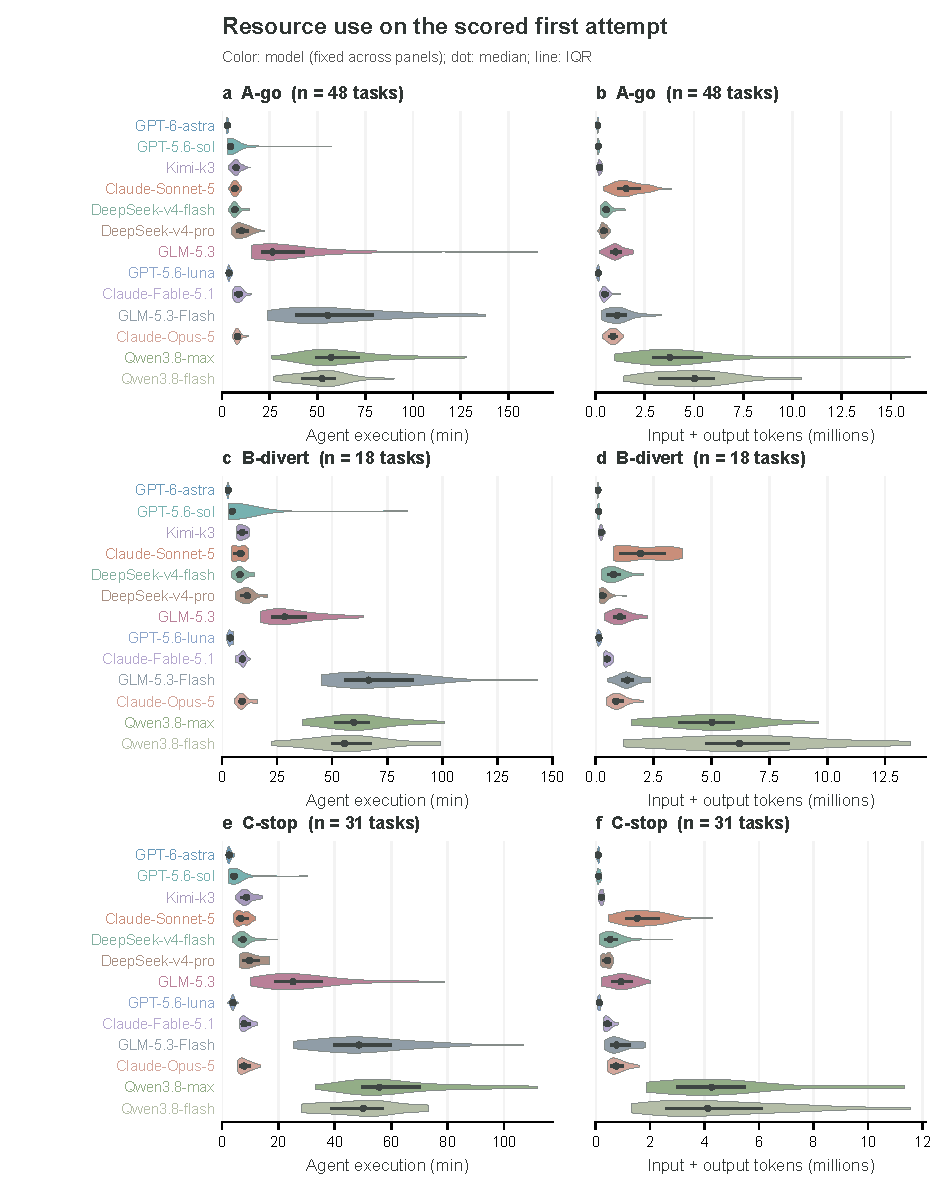
\includegraphics[width=\linewidth]{figures/figure06_resource_distributions.pdf}
\caption{\textbf{Execution-time and token distributions.} Rows separate A-go (48 tasks), B-divert (18) and C-stop (31); each agent contributes its first scored attempt. Each model has a fixed color across all six panels. Violin width shows a kernel density estimate within the observed range; dots mark medians and thick lines the interquartile range, not confidence intervals. Axes start at zero and use panel-specific ranges. Any incomplete telemetry is labelled observed/total beside the corresponding violin. All agents use the same harness, so we retain individual agents rather than pool by harness.}
\label{fig:appendix-resources}
\end{figure}

\paragraph{Model-level summaries.}
All 1,261 scored first attempts (13 agents $\times$ 97 tasks) have execution timestamps and token counts. Table~\ref{tab:runtime-summary} summarizes the observed time distribution. Medians range from 2.7 minutes for GPT-6-astra to 58.2 for Qwen3.8-max, while cumulative agent execution ranges from 4.4 to 101.3 hours per agent. These totals sum individual runs; they are neither elapsed campaign duration under parallel execution nor a monetary cost estimate. For GPT-5.6-sol, a 4.4-minute median accompanies a maximum of 84.0 minutes. One GLM-5.3 run, case 29 seed 2, ended with an agent-timeout exception at 144.0 minutes. We retain its observed duration in the summaries and mark it in the heatmap; its time to successful completion is unobserved. Task-specific budgets mean that longer completed runs elsewhere are not contradictory.

\begin{table}[!htbp]
\caption{\textbf{Observed execution time per agent.} Each row contains the same 97 first-attempt tasks. Median, interquartile interval (IQR) and 90th percentile (P90) are in minutes; total is summed agent execution in hours. TO counts agent-timeout exceptions. Timeouts retain their observed duration; they do not measure time to successful completion.}
\label{tab:runtime-summary}
\centering
\small
\begin{tabular}{@{}lrrrrr@{}}
\toprule
Agent & Median & IQR & P90 & Total (h) & TO \\
\midrule
GPT-6-astra & 2.7 & 2.4--3.1 & 3.5 & 4.4 & 0 \\
GPT-5.6-sol & 4.4 & 4.0--4.9 & 7.9 & 10.7 & 0 \\
Kimi-k3 & 7.9 & 6.8--9.4 & 11.5 & 13.3 & 0 \\
Claude-Sonnet-5 & 6.7 & 5.6--8.6 & 9.6 & 11.6 & 0 \\
DeepSeek-v4-flash & 7.2 & 6.1--8.4 & 12.2 & 12.6 & 0 \\
DeepSeek-v4-pro & 10.4 & 8.2--13.0 & 16.4 & 17.7 & 0 \\
GLM-5.3 & 26.5 & 20.6--37.6 & 60.0 & 54.9 & 1 \\
GPT-5.6-luna & 3.7 & 3.3--4.3 & 4.9 & 6.1 & 0 \\
Claude-Fable-5.1 & 8.7 & 7.2--9.9 & 11.2 & 14.2 & 0 \\
GLM-5.3-Flash & 54.2 & 42.8--73.0 & 92.6 & 97.9 & 0 \\
Claude-Opus-5 & 8.4 & 7.2--9.2 & 11.4 & 13.9 & 0 \\
Qwen3.8-max & 58.2 & 49.7--70.9 & 91.5 & 101.3 & 0 \\
Qwen3.8-flash & 52.4 & 42.1--60.4 & 71.3 & 84.6 & 0 \\
\bottomrule
\end{tabular}

\end{table}

\paragraph{Model by task.}
Figure~\ref{fig:runtime-tasks} retains individual task identity, with the same case-and-seed ordering as the route-success heatmaps in Appendix~\ref{app:reliability}. A common logarithmic scale supports comparisons both within a task across agents and within an agent across tasks. Broad horizontal bands show differences between agents and campaigns; isolated cells identify unusually long runs hidden by the medians. The panel separates reference routing tiers rather than pooling tasks requiring continuation with tasks requiring diversion or termination. These comparisons are descriptive: model, provider latency, execution date and attempted work vary together.

\begin{figure}[!htbp]
\centering
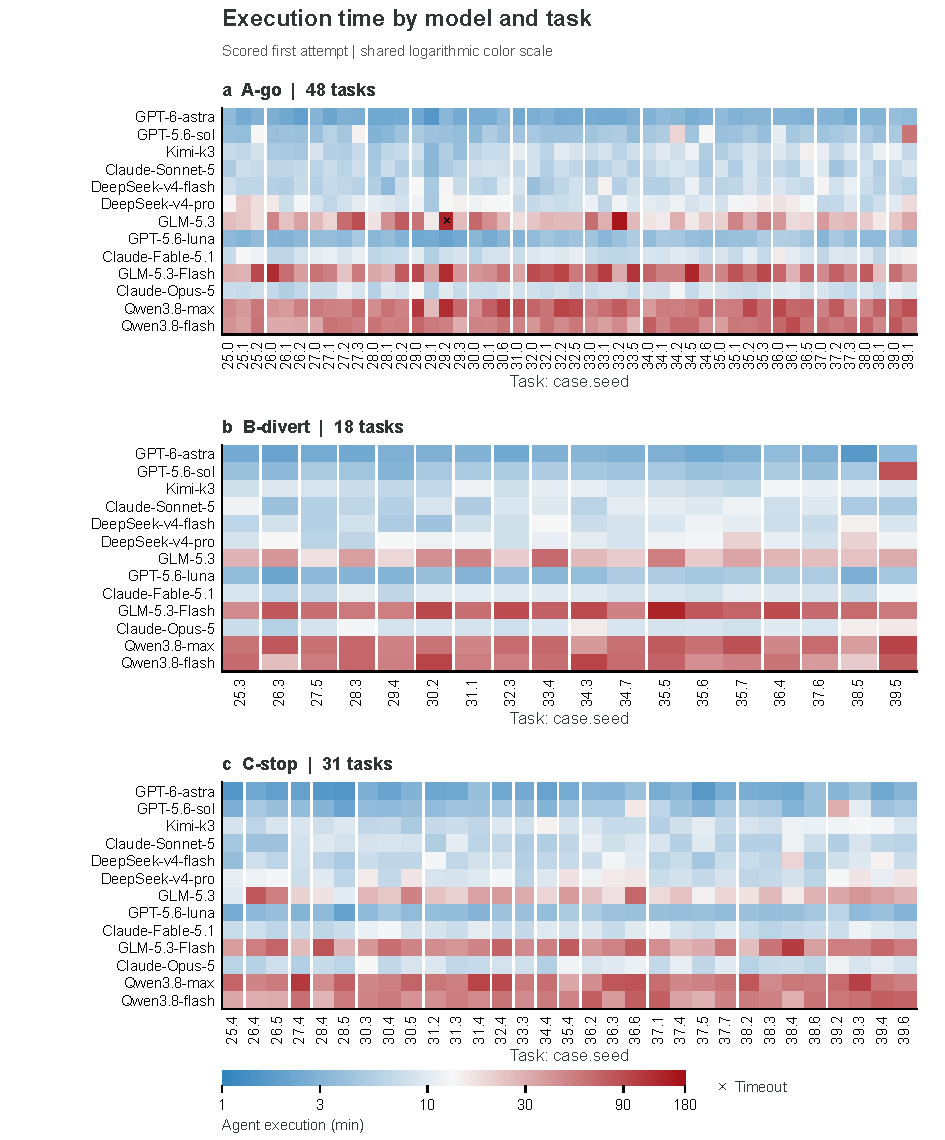
\includegraphics[width=\linewidth]{figures/figure07_runtime_by_task.pdf}
\caption{\textbf{Execution time by model and task.} One cell is one scored first attempt. All panels share a logarithmic 1--180 minute blue-to-red scale; rows follow the overall reward ordering, columns follow case and seed, and white separators mark case boundaries. The cross marks the sole agent-timeout exception. Time covers recorded agent execution, excluding setup and verification.}
\label{fig:runtime-tasks}
\end{figure}

\paragraph{Does correct stopping use fewer resources?}
Among 403 C-stop runs, 100 have every graded route decision correct, 282 contain forbidden no-go work (E1), and 21 meet neither definition. Figure~\ref{fig:runtime-stop} compares the first two disjoint groups within each agent; their tasks differ, and the excluded runs include other routing failures. The correct group has lower median execution time in only 6 of 13 agents. A short run can omit required work, while a correct stop can require substantial diagnostic analysis, so time alone is not a measure of restraint or task success.

To reduce case-mix differences, we also compare seeds within each model--case group containing both outcomes: 38 groups across all 13 agents, but only five cases. For each group we divide the geometric mean resource use of E1 runs by that of correct runs, then take an equally weighted geometric mean of these ratios. The ratios are 1.12 for execution time and 1.07 for input-plus-output tokens. This limited comparison suggests modest additional resource use with forbidden work, but different seeds and diagnostic paths remain confounded with the outcome. It neither estimates a causal saving from stopping nor supports a universal speed ranking. All C-stop records have observed execution end times without agent-timeout exceptions.

\begin{figure}[!htbp]
\centering
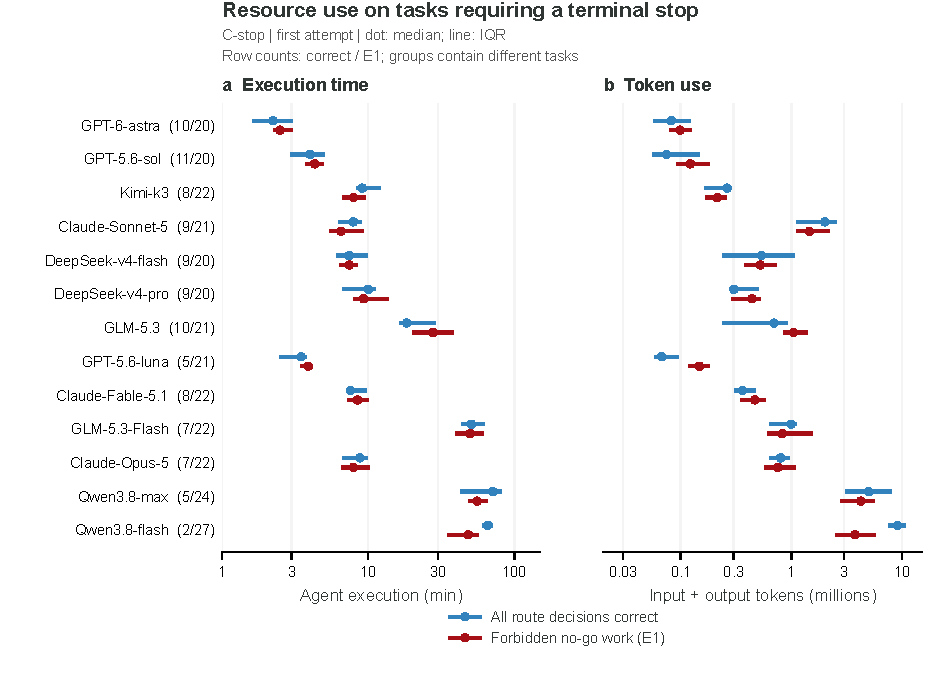
\includegraphics[width=\linewidth]{figures/figure08_stop_task_resources.pdf}
\caption{\textbf{Resources and route correctness on C-stop tasks.} Blue: all graded route decisions correct; red: at least one E1 error. Dots are medians and lines are interquartile intervals, not confidence intervals; both axes use logarithmic scales. Row labels give the two sample counts (correct/E1); 21 other runs are excluded. Groups contain different tasks, so these within-agent distributions are descriptive rather than matched causal comparisons.}
\label{fig:runtime-stop}
\end{figure}


\section{Worked example: case 33}
\label{app:example}

\textbf{The problem.} An electronic-assembly line accepts or rejects boards by eye at
final inspection and must hold its reject share at or below 2\%. The improvement team
has five sets of records: the inspected and rejected counts of twenty-five
consecutive lots; a study in which several inspectors judged the same retained boards
against an agreed answer key; a tally of the items those inspectors called differently
from the key, by reject category; a second study on retained boards run after the
accept/reject criteria were rewritten; and one window's placed and rejected counts for
each of two placement heads. The agent is asked to report where the project stands:
whether an accept/reject call can be relied on, what had to happen before it could be,
whether the reject share has held steady across the lots, how today's level compares with
the requirement, and what should be done next. Every reported number must come from a computation the agent ran
(the instruction is Listing~\ref{lst:c33}).

\textbf{Sequential decisions.} The data steward releases one batch per request in the order fixed by the protocol: the tally only after the first
study, the second study only after the tally, the lot record only after a study, the head
counts only after the lots. Earlier results also determine the valid analysis at each stage: whether the first study passes decides whether the
project goes to the lot record or to the tally and a second study; whether the second
study passes decides whether the project continues or ends with an escalation; whether the
lot chart is stable decides whether a capability index may be computed at all; whether the
level is met decides whether a cause is sought. A complete walk is eight analyses over
five phases, about ten steward exchanges, a dozen agent turns and a written report; on
some data the correct walk is four analyses and a report that says why the rest was not
done. The agent must carry diagnostic results forward to choose the correct route.

Case 33 is public and draws on a practitioner project (\S\ref{sec:unit}). Its graph (Figure~\ref{fig:c33-graph}) has eleven nodes, with the route determined by three computed values. Seed 2 is the long walk: the first inspector study
fails, the rewritten criteria are proved, the lot record is stable, the reject share
misses the requirement, one placement head is found to differ, and the project improves
and moves to control. Seed 3 is the same case with different data: the rewritten
criteria are \emph{not} proved, and the correct project ends at its fourth analysis. We compare GPT-6-astra on both seeds (Table~\ref{tab:c33-timeline}), including each turn, released batch, and reference and expert decision at each fork. The following sections give the case and verifier package, the same agent under \emph{permit-stop}, and all agents on seed 3. We reproduce the complete plain seed-2 and \emph{permit-stop} seed-3 reports.

In Figure~\ref{fig:c33-graph}, nodes are analyses coloured by phase (Table~\ref{tab:c33-nodes}); double borders mark terminal nodes. Edge labels specify guards, with {default} used when none holds. Their shared prefix is purple.

\begin{figure}[!ht]
\centering
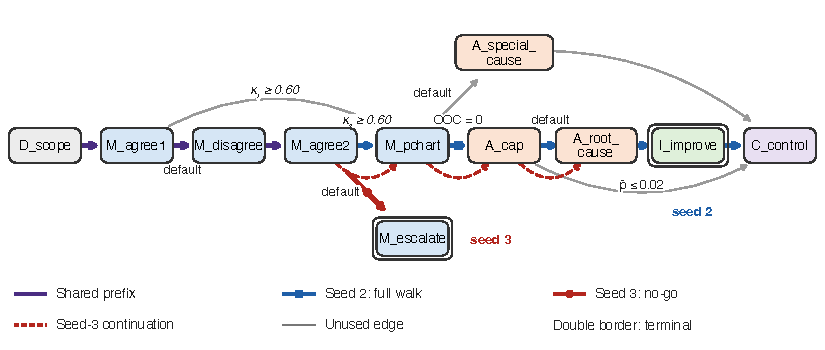
\includegraphics[width=\linewidth]{figures/figure09_case33_routes.pdf}
\caption{\textbf{Case 33 and its two reference routes.} Blue squares trace seed 2 through all five phases; red circles trace seed 3 to M\_escalate. Red dashes trace seed 3 past measurement failure.}
\label{fig:c33-graph}
\end{figure}

\subsection{Project narrative}

Table~\ref{tab:c33-timeline} pairs each trace step with the steward interaction that released its batch and the guard evaluated on its output. Step 7 of seed 2 is an extra test absent from the reference route: it lowers method precision without constituting a wrong turn. On seed 3, the second study fails its guard, but the run requests the lot record and performs four analyses on the closed branch.

\FloatBarrier
\begingroup
\fontsize{8}{9.5}\selectfont
\setlength{\tabcolsep}{2pt}
\begin{longtable}{@{}R{0.04\linewidth}P{0.13\linewidth}P{0.16\linewidth}P{0.14\linewidth}P{0.17\linewidth}P{0.16\linewidth}P{0.135\linewidth}@{}}
\caption{GPT-6-astra on case 33, seeds 2 and 3, under the plain instruction (first attempt). Trace steps list released batches, reported values, guards and branches. \checkmark: correct fork; $\times$: incorrect fork.}\label{tab:c33-timeline}\\
\toprule
Step & Node & Batch (steward \#) & Analysis & Reported value & Guard read on it & Route taken \\
\endfirsthead
\multicolumn{7}{c}{\normalfont\normalsize Table \thetable{} (continued)} \\
\noalign{\vskip 6pt}
\toprule
Step & Node & Batch (steward \#) & Analysis & Reported value & Guard read on it & Route taken \\
\midrule
\endhead
\bottomrule
\endfoot
\midrule
\multicolumn{7}{@{}l}{\textbf{Seed 2: the study fails, the repair holds, the level is missed --- the full walk (tier A)}} \\*
\midrule
1 & D\_scope & \texttt{define} (\#3) & read the charter & required share 0.02 &  & $\to$ M\_agree1 \\
2 & M\_agree1 & \texttt{study\_1} (\#2) & attribute agreement & $\kappa_{\min}$ 0.2857, agreement 73.33\% & $\kappa_1 \geq 0.60$: fails & $\to$ M\_disagree \checkmark \\
3 & M\_disagree & \texttt{disagreements} (\#6) & Pareto of disagreements & top category 47.78\% &  & $\to$ M\_agree2 \\
4 & M\_agree2 & \texttt{study\_2} (\#7) & attribute agreement & $\kappa_{\min}$ 0.9419, agreement 99.17\% & $\kappa_2 \geq 0.60$: holds & $\to$ M\_pchart \checkmark \\
5 & M\_pchart & \texttt{lots} (\#8) & $p$ chart & CL 0.0311, out of limits 0 & OOC $= 0$: holds & $\to$ A\_cap \checkmark \\
6 & A\_cap & \texttt{lots} & binomial capability & $\bar p$ 0.0311, $Z$ 1.865 & $\bar p \leq 0.02$: fails & $\to$ A\_root\_cause \checkmark \\
7 & --- & \texttt{lots} & one-proportion test & $p$ = 1.3e$-$13 &  & \emph{off route} \\
8 & A\_root\_cause & \texttt{heads} (\#9) & two-proportion test & 4.27\% vs 2.47\%, $p$ = 0.00011 &  & $\to$ I\_improve (terminal), then C\_control \\
\midrule
\multicolumn{7}{@{}l}{\textbf{Seed 3: the study fails, the repair fails --- the walk that must stop (tier C)}} \\*
\midrule
1 & M\_agree1 & \texttt{study\_1} (\#2) & attribute agreement & $\kappa_{\min}$ 0.4581, agreement 81.67\% & $\kappa_1 \geq 0.60$: fails & $\to$ M\_disagree \checkmark \\
2 & M\_disagree & \texttt{disagreements} (\#5) & Pareto of disagreements & top category 46.67\% &  & $\to$ M\_agree2 \\
3 & M\_agree2 & \texttt{study\_2} (\#6) & attribute agreement & $\kappa_{\min}$ 0.5455, agreement 79.17\% & $\kappa_2 \geq 0.60$: fails & correct: $\to$ M\_escalate, the project ends; taken: went on $\times$ \\
4 & M\_pchart & \texttt{lots} (\#8) & $p$ chart & CL 0.0125, out of limits 1 & --- & \emph{past the closed fork} \\
5 & A\_cap & \texttt{lots} & binomial capability & $\bar p$ 0.0125, $Z$ 2.241 & --- & \emph{past the closed fork} \\
6 & --- & \texttt{lots} & one-proportion test & $p$ = 6.1e$-$09 & --- & \emph{past the closed fork} \\
7 & A\_root\_cause & \texttt{heads} (\#10) & two-proportion test & 1.87\% vs 1.63\%, $p$ = 0.49 & --- & \emph{past the closed fork} \\
\end{longtable}
\par\normalsize\noindent\textbf{Run accounting.} Seed 2: 9 steward interactions (6 batches released, 2 refused), 8 trace steps, 27 report lines, 3 min 4 s wall clock; pq 4/4, ms\_precision 0.857, reward 0.960.\par\noindent Seed 3: 10 steward interactions (6 batches released, 3 refused), 7 trace steps, 32 report lines, 3 min 2 s wall clock; pq 1/2, ms\_precision 0.333, reward 0.571.\par

\endgroup

On seed 2 the run follows the reference route: nine steward interactions, of which one
{provision} (asking the plant for an agreement threshold) was refused as
{firewall} and one request was {unroutable} until rephrased; eight
analyses, every guard field reported within tolerance, all four forks right, and a
five-section report that qualifies the inspection, states the stable-but-noncompliant
level, names the outlying head and hands over a control plan
(Listing~\ref{lst:c33-s2-report}). The decision at A\_cap (step 6) depends on the verdicts at steps 2, 4 and 5. The report's recommendation relies on step 8, whose execution requires a valid prerequisite verdict from the analysis at step 6.

Seed 3 begins with the same three analyses but produces different results: the
rewritten criteria reach $\kappa_{\min} = 0.5455$, below the guard. The run states this
(``the rewrite did \textbf{not} establish a reliable measurement system''), then requests
the lot record and runs the $p$ chart, the capability index and two proportion tests
that belong to the branch the study had closed. Both forks of seed 3 are graded; the
second is scored \emph{incorrect via divergent evidence}, reward 0.571 against 0.960 on
seed 2: changing the second measurement verdict requires this agent to take a different route through the same case.

\subsection{Turn-level transcripts of two runs}

Table~\ref{lst:c33-s3-turns} is the seed-3 run turn by turn, in the agent's own words:
at turn 7 it writes ``Rewritten criteria did not validate measurement \ldots{} Declare
measurement failure honestly; do not treat released data as proof of validity'', tries a
declaration the case has no lock for, and in the same command requests the placement-head
counts; at turn 8, ``the failed validation remains the decisive project finding'', it
computes the $p$ chart, the capability index and the two tests and plans to ``label them
non-certifying''. The agent describes the diagnostic correctly at each turn but then performs analyses that the diagnostic rules out. Table~\ref{lst:c33-s2-turns} is the seed-2 run in the same form,
for comparison: the same opening, followed by analyses that the earlier diagnostic results on the reference route permit.

The transcript tables reproduce each turn's analysis and plan verbatim on the left. On the right are steward calls and replies, released batch contents in grey, coded analyses and their printed guard fields; re-runs are omitted. Shaded fork rows show the computed guard, reference route, expert majority where study 2 sampled the seed and fork, and the agent's action. Green marks agreement with the route and red a departure; red turn rows identify where the run went off route.

\FloatBarrier
{\small\setlength{\tabcolsep}{0pt}\renewcommand{\arraystretch}{1.15}
\begin{longtable}{@{}r@{\hskip 6pt}>{\raggedright\arraybackslash}p{0.42\linewidth}@{\hskip 8pt}>{\raggedright\arraybackslash}p{0.48\linewidth}@{}}
\caption{GPT-6-astra, seed 3, plain instruction, by turn. Left: verbatim analysis and plan. Right: steward exchanges and executed analyses. Shading marks route decisions.}\label{lst:c33-s3-turns}\\
\toprule
Turn & The agent's stated analysis and plan & What it did, and what came back \\
\midrule
\endfirsthead
\multicolumn{3}{c}{\normalfont\normalsize Table \thetable{} (continued)} \\
\noalign{\vskip 6pt}
\toprule
Turn & The agent's stated analysis and plan & What it did, and what came back \\
\midrule
\endhead
\bottomrule
\endfoot
\rowcolor{gray!7}1 & No batches have been obtained yet. \emph{Plan: Check availability and request the initial inspector agreement study before assessing process performance.} & \texttt{status}: two batches available, four locked \newline \texttt{request} ``initial inspector attribute agreement study against the answer key'' $\to$ released \texttt{study\_1} \newline \quad\textcolor{gray!70!black}{data: 3 appraisers $\times$ 2 repeats $\times$ 20 boards, pass/fail, with the answer key} \\
2 & The initial repeated ratings are available; agreement must be computed before trusting rejection data. \emph{Plan: Inspect JSON structure and charter, then compute agreement against the reference.} & reads \texttt{study\_1.json} \newline \texttt{request} ``Project charter and required reject level'' $\to$ released \texttt{define} \newline \quad\textcolor{gray!70!black}{data: the goal and the required share 0.02} \\
\rowcolor{gray!7}3 & The study contains repeated binary ratings and a reference vector. \emph{Plan: Create a reusable analysis/trace script, compute per-inspector pooled Cohen kappa and agreement, then request disagreement categories.} & codes attribute agreement \newline runs attribute agreement $\to$ $\kappa_{\min}$ 0.4581, agreement 81.67\% \newline \texttt{request} ``Items called differently from the key by reject category'' $\to$ refused (\texttt{unroutable}) \\
\rowcolor{green!10}\multicolumn{3}{@{}p{\linewidth}@{}}{\small \textbf{Fork M\_agree1}: $\kappa_1 \geq 0.60$ reads 0.4581, fails. Reference route $\to$ M\_disagree. human experts: no study-2 unit at this fork. agent: the same \checkmark} \\
4 & Initial minimum kappa is about 0.458, so calls are not yet dependable. The category request was unroutable, not a denial. \emph{Plan: Retry with the advertised topic wording.} & \texttt{request} ``disagreement tally'' $\to$ released \texttt{disagreements} \newline \quad\textcolor{gray!70!black}{data: 90 items in 5 categories (insufficient solder 42, tombstone 17, component offset 14, solder bridge 9, wrong polarity 8)} \\
\rowcolor{gray!7}5 & Category tally is released and can prioritize clarification, but is not a production-defect Pareto. \emph{Plan: Compute category shares and request the post-rewrite validation study and the process fact on the rewrite.} & runs Pareto of the disagreements $\to$ top category 46.67\% \newline \texttt{request} ``second study rewritten criteria'' $\to$ released \texttt{study\_2} \newline \quad\textcolor{gray!70!black}{data: 3 appraisers $\times$ 2 repeats $\times$ 20 boards, pass/fail, with the answer key} \newline \texttt{provision} ``What specifically was changed in the accept/reject criteria and inspector training between the initial and second studies?''  \newline \quad $\to$ refused (\texttt{unroutable}) \\
\rowcolor{red!9}6 & The validation study is available, but visual inspection suggests disagreements remain. The process-owner reply is pending. \emph{Plan: Compute validation agreement and inspect the response before proceeding.} & runs attribute agreement $\to$ $\kappa_{\min}$ 0.5455, agreement 79.17\% \newline \texttt{request} ``lot record boards inspected per lot lot order'' $\to$ released \texttt{lots} \newline \quad\textcolor{gray!70!black}{data: 25 lots of 400: rejects 4, 6, 4, 10, 5, 4, 5, 3, 0, 6, 3, 3, 5, 3, 3, 3, 5, 5, 3, 9, 8, 4, 5, 12, 7} \\
\rowcolor{red!14}\multicolumn{3}{@{}p{\linewidth}@{}}{\small \textbf{Fork M\_agree2}: $\kappa_2 \geq 0.60$ reads 0.5455, fails. Reference route $\to$ M\_escalate, the project ends here. human experts (study 2, majority of three, reading DeepSeek-v4-pro's run of this seed and fork): NO-GO. agent: requests \texttt{lots} at turn 6 and runs the $p$ chart at turn 8 $\times$} \\
\rowcolor{gray!7}7 & Rewritten criteria did not validate measurement: minimum kappa remains low and pooled agreement fell. Lot records are available, but any process assessment must be explicitly provisional. \emph{Plan: Inspect lot structure and request placement-head counts. Declare measurement failure honestly; do not treat released data as proof of validity.} & \texttt{declare} \texttt{measurement\_valid} $\to$ refused: no such lock on this case \newline reads \texttt{lots.json} \newline \texttt{request} ``placement heads head by head'' $\to$ released \texttt{heads} \newline \quad\textcolor{gray!70!black}{data: 56 of 3,000 and 49 of 3,000} \\
\rowcolor{red!9}8 & Both process batches are available without gates, but the failed validation remains the decisive project finding. \emph{Plan: Compute descriptive conditional p-chart, binomial performance and head comparison, label them non-certifying, and write the required report and trace.} & codes $p$ chart, binomial capability, one-proportion test, two-proportion test \newline runs $p$ chart $\to$ centre line 0.0125, 1 lot(s) out of limits \newline runs binomial capability $\to$ $\bar p$ 0.0125, $Z$ 2.241 \newline runs one-proportion test $\to$ $p$ = 6.1e-09 \newline runs two-proportion test $\to$ 1.87\% vs 1.63\%, $p$ = 0.49 \\
\rowcolor{gray!7}9 & The computed chart actually flags a lot; both unstable recorded performance and inadequate inspection prevent capability certification. Head comparison does not establish a difference. \emph{Plan: Correct the chart narrative to match computation, record the flagged lot, and produce the manager report with numerical provenance.} & writes the report (22 lines) \\
10 & Both required files exist and trace.json parses successfully. The report distinguishes inadequate inspection validation, a flagged historical lot, nominal recorded performance below the ceiling, and an inconclusive placement-head comparison. All reported numerical results derive from computations saved in the trace. \emph{Plan: No further actions are required.} & marks the task complete \\
\rowcolor{gray!7}11 & The required report and computation trace have been written and checked. Conclusions explicitly retain the failed measurement-validation limitation and do not claim successful process capability. \emph{Plan: Finalize the submitted files.} & marks the task complete \\
\midrule
\multicolumn{3}{@{}l}{\emph{11 agent turns, 108,566 prompt and 3,275 completion tokens, \$0.43; pq 1/2, reward 0.571.}} \\
\end{longtable}

\begin{longtable}{@{}r@{\hskip 6pt}>{\raggedright\arraybackslash}p{0.42\linewidth}@{\hskip 8pt}>{\raggedright\arraybackslash}p{0.48\linewidth}@{}}
\caption{GPT-6-astra on seed 2, plain instruction, turn by turn (same conventions).}\label{lst:c33-s2-turns}\\
\toprule
Turn & The agent's stated analysis and plan & What it did, and what came back \\
\midrule
\endfirsthead
\multicolumn{3}{c}{\normalfont\normalsize Table \thetable{} (continued)} \\
\noalign{\vskip 6pt}
\toprule
Turn & The agent's stated analysis and plan & What it did, and what came back \\
\midrule
\endhead
\bottomrule
\endfoot
\rowcolor{gray!7}1 & We need obtain the initial measurement study and learn release criteria before judging the process. \emph{Plan: Check status and request the baseline inspector agreement data.} & \texttt{status}: two batches available, four locked \newline \texttt{request} ``initial attribute agreement study: inspectors versus retained board answer key'' $\to$ released \texttt{study\_1} \newline \quad\textcolor{gray!70!black}{data: 3 appraisers $\times$ 2 repeats $\times$ 20 boards, pass/fail, with the answer key} \\
2 & Initial repeated ratings are released; we need compute agreement against standard and inspect stored structure. \emph{Plan: Read JSON layout, charter, and process acceptance criterion.} & reads \texttt{study\_1.json} \newline \texttt{request} ``project charter required reject level'' $\to$ released \texttt{define} \newline \quad\textcolor{gray!70!black}{data: the goal and the required share 0.02} \newline \texttt{provision} ``What criterion should be used to accept inspector attribute agreement against the answer key?'' $\to$ refused (\texttt{firewall}) \\
\rowcolor{gray!7}3 & We have full baseline ratings and required reject share. The owner did not supply additional process facts. \emph{Plan: Compute pooled per-appraiser Cohen kappa and observed agreement, recording all results; then request disagreement categories.} & codes attribute agreement, data profile \newline computes attribute agreement $\to$ $\kappa_{\min}$ 0.2857, agreement 73.33\% \newline \texttt{request} ``Items called differently from the key by reject category'' $\to$ refused (\texttt{unroutable}) \\
\rowcolor{green!10}\multicolumn{3}{@{}p{\linewidth}@{}}{\small \textbf{Fork M\_agree1}: $\kappa_1 \geq 0.60$ reads 0.2857, fails. Reference route $\to$ M\_disagree. human experts: no study-2 unit at this fork. agent: the same \checkmark} \\
4 & Baseline agreement is poor: minimum kappa about 0.286. Category request was unroutable, not denied. \emph{Plan: Use the exact routing topic to obtain the disagreement tally.} & \texttt{request} ``disagreement tally'' $\to$ released \texttt{disagreements} \newline \quad\textcolor{gray!70!black}{data: 90 items in 5 categories (insufficient solder 43, tombstone 16, component offset 13, wrong polarity 11, solder bridge 7)} \\
\rowcolor{gray!7}5 & Disagreements concentrate in insufficient solder, but this is measurement error rather than proof of process defect causes. \emph{Plan: Compute Pareto percentages and request the rewritten-criteria study.} & reads \texttt{disagreements.json} \\
6 & The command batch is still executing. \emph{Plan: Wait for the follow-up study release.} & \texttt{request} ``second study rewritten criteria'' $\to$ released \texttt{study\_2} \newline \quad\textcolor{gray!70!black}{data: 3 appraisers $\times$ 2 repeats $\times$ 20 boards, pass/fail, with the answer key} \\
\rowcolor{gray!7}7 & The follow-up data are available after the criteria rewrite. \emph{Plan: Compute agreement again and request lot history.} & \texttt{request} ``lot record boards inspected per lot lot order'' $\to$ released \texttt{lots} \newline \quad\textcolor{gray!70!black}{data: 25 lots of 400: rejects 12, 12, 9, 20, 13, 12, 15, 12, 15, 12, 17, 15, 15, 17, 13, 13, 18, 8, 9, 8, 10, 8, 16, 7, 5} \newline computes attribute agreement $\to$ $\kappa_{\min}$ 0.9419, agreement 99.17\% \\
\rowcolor{green!10}\multicolumn{3}{@{}p{\linewidth}@{}}{\small \textbf{Fork M\_agree2}: $\kappa_2 \geq 0.60$ reads 0.9419, holds. Reference route $\to$ M\_pchart. human experts: no study-2 unit at this fork. agent: the same \checkmark} \\
8 & Rewritten criteria produced strong agreement. Lot counts allow a binomial p chart and capability relative to required share. \emph{Plan: Inspect layout and compute control limits, binomial capability and target test; obtain head comparison.} & reads \texttt{lots.json} \\
\rowcolor{gray!7}9 & All lot sizes are equal; reject counts represent boards, so a p chart is appropriate rather than a continuous capability index. \emph{Plan: Compute and save lot analyses then request heads.} & codes $p$ chart, binomial capability, one-proportion test \newline computes $p$ chart $\to$ centre line 0.0311, 0 lot(s) out of limits \newline computes binomial capability $\to$ $\bar p$ 0.0311, $Z$ 1.865 \newline computes one-proportion test $\to$ $p$ = 1.3e-13 \newline \texttt{request} ``placement heads head by head'' $\to$ released \texttt{heads} \newline \quad\textcolor{gray!70!black}{data: 128 of 3,000 and 74 of 3,000} \\
\rowcolor{green!10}\multicolumn{3}{@{}p{\linewidth}@{}}{\small \textbf{Fork M\_pchart}: OOC $= 0$ reads 0, holds. Reference route $\to$ A\_cap. human experts (study 2, majority of three, reading GLM-5.3's run of this seed and fork): NO-GO --- one of the four go-side disagreements of \S\ref{sec:study2}. agent: the same \checkmark} \\
\rowcolor{green!10}\multicolumn{3}{@{}p{\linewidth}@{}}{\small \textbf{Fork A\_cap}: $\bar p \leq 0.02$ reads 0.0311, fails. Reference route $\to$ A\_root\_cause. human experts: no study-2 unit at this fork. agent: the same \checkmark} \\
10 & Lot history shows a stable point-limit chart but excessive rejection. Head counts can identify an association, not establish a mechanical cause. \emph{Plan: Test head proportions, record route decisions, and write the manager report with traceable results and explicit limitations.} & codes two-proportion test \newline runs two-proportion test $\to$ 4.27\% vs 2.47\%, $p$ = 0.00011 \\
\rowcolor{gray!7}11 & Both required files exist and the trace parses as JSON. The report covers measurement qualification, disagreement priorities, lot stability, failure to meet the reject requirement, and placement-head evidence, while distinguishing association from root cause and measurement improvement from production improvement. \emph{Plan: No further commands are needed; deliver the completed report and computation trace.} & marks the task complete \\
12 & The required report and trace have been written and verified. All reported quantitative findings are supported by computations recorded in the trace. \emph{Plan: Confirm completion.} & marks the task complete \\
\midrule
\multicolumn{3}{@{}l}{\emph{12 agent turns, 115,775 prompt and 3,295 completion tokens, \$0.58; pq 4/4, reward 0.960.}} \\
\end{longtable}
}


\Needspace{8\baselineskip}
\subsection{Case specification}
\noindent
The contestant reads this and nothing else about the project:

\begin{lstlisting}[caption={Sections 1 and 2 of the instruction for case 33.},label={lst:c33}]
## 1. Business background
We are the improvement team on an electronic-assembly line. Boards are
accepted or rejected by eye at final inspection, and the line is
required to hold the reject share at or below 2%
the inspected and rejected counts for twenty-five consecutive lots, a
study in which several inspectors judged the same retained boards
against an agreed answer key, a tally of the items those inspectors
called differently from the key broken out by the category the item
was rejected under, a second study run on retained boards after the
accept/reject criteria were rewritten, and one window's rejected and
placed counts for each of the two placement heads.

## 2. What you are asked to do
Work through the batches the data steward will release and report
where this project stands: whether an accept/reject call can be relied
on, what had to happen before it could be, whether the reject share
has held steady across the lots, how today's level compares with what
the line is required to hold, and what should be done next. Every
number in your report must come from a computation you ran on this
task; where something could not be computed, say so rather
than inventing it.
\end{lstlisting}
\par\medskip

The source project measured visual-judgment agreement at $\kappa = 0.44$, rewrote the criteria and repeated the study at $1.00$. The case retains the requirement to validate the repair, while generating its own data. Rewriting the criteria establishes that they changed; a second study must establish whether they now work, and that study can fail. Every other measurement-system case in the corpus stops at a failed study. Case 33 tests the initial failure and whether the repair succeeds.

\begin{table}[!htbp]
\caption{Nodes of case 33.}
\label{tab:c33-nodes}
\centering
\footnotesize
\setlength{\tabcolsep}{3pt}
\begin{tabular}{@{}llllP{0.26\linewidth}@{}}
\toprule
Node & Phase & Method & Produces & Description \\
\midrule
D\_scope         & define  & ---                          & ---                     & the reject share at visual inspection and its required level \\
M\_agree1        & measure & msa.attribute\_agreement     & agree1.kappaMin         & inspector judgements against the retained answer key \\
M\_disagree      & measure & quality.pareto               & disagree.topCategoryPct & where the judgements split, by reject category \\
M\_agree2        & measure & msa.attribute\_agreement     & agree2.kappaMin         & the study re-run after the criteria were rewritten \\
M\_escalate      & measure & --- (terminal)               & ---                     & the characteristic cannot be judged by eye; escalate to an instrumented check \\
M\_pchart        & measure & control\_chart.p             & pchart.outOfControl     & lot-by-lot reject share across the record \\
A\_special\_cause & analyze & control\_chart.p            & ---                     & special-cause investigation \\
A\_cap           & analyze & capability.binomial          & cap.avgP                & the reject share against the required level \\
A\_root\_cause   & analyze & basic.two\_proportions       & rootcause.pValue        & the two placement heads compared \\
I\_improve       & improve & --- (terminal)               & ---                     & bring the outlying head onto the other's level \\
C\_control       & control & control\_chart.p             & ---                     & attribute-chart monitoring \\
\bottomrule
\end{tabular}

\end{table}

\begin{table}[!htbp]
\caption{Edges of case 33. Four forks; the two on the measurement studies read the
same method twice, so the truth pins each verdict to its invocation.}
\label{tab:c33-edges}
\centering
\footnotesize
\begin{tabular}{@{}llP{0.32\linewidth}@{}}
\toprule
Edge & Guard & Interpretation \\
\midrule
D\_scope $\to$ M\_agree1             & ---                              & \\
M\_agree1 $\to$ M\_pchart            & \texttt{agree1.kappaMin >= 0.60} & study acceptable \\
M\_agree1 $\to$ M\_disagree          & default                          & study fails: find what the calls split on \\
M\_disagree $\to$ M\_agree2          & ---                              & \\
M\_agree2 $\to$ M\_pchart            & \texttt{agree2.kappaMin >= 0.60} & the repair is proved \\
M\_agree2 $\to$ M\_escalate          & default                          & the repair is not proved: NO-GO \\
M\_pchart $\to$ A\_cap               & \texttt{pchart.outOfControl == 0} & stable: the share is one number \\
M\_pchart $\to$ A\_special\_cause    & default                          & unstable: DIVERT \\
A\_cap $\to$ C\_control              & \texttt{cap.avgP <= 0.02}        & meets the required level \\
A\_cap $\to$ A\_root\_cause          & default                          & misses it \\
A\_special\_cause $\to$ C\_control & --- & \\
A\_root\_cause $\to$ I\_improve & --- & \\
I\_improve $\to$ C\_control & --- & \\
\bottomrule
\end{tabular}

\end{table}

The steward holds six batches: the charter ({define}), the first study
({study\_1}), the disagreement tally ({disagreements}, requires
{study\_1}), the second study ({study\_2}, requires
{disagreements}), the lot record ({lots}, requires either study), and the
head-by-head counts ({heads}, requires {lots}). All six locks are order
locks: the agreement criterion has no public form, so the lot record is released once a
study exists, whatever its verdict. The contestant must use $\kappa$ to decide whether lot charting is valid.

\subsection{Seeds and task variants}

Table~\ref{tab:c33-seeds} lists the six tasks the case generates: the same graph, six
data sets, four correct routes of three tiers, and one seed (3) on which the correct
project ends after four analyses. The columns $\kappa_1$ and $\kappa_2$ give the minimum appraiser agreement in the first and second studies; the second study exists only when the first fails. OOC counts lots beyond the $p$-chart limits, and $\bar p$ is the average reject share compared with the required 0.02. Seed 3 has one lot beyond the limits and a share below that requirement, but its failed measurement study makes those downstream calculations invalid.

\begin{table}[!htbp]
\caption{The six tasks generated by case 33, with diagnostic values and correct routes. Seed 3 requires stopping after the revised inspection criteria fail to establish reliable measurements.}
\label{tab:c33-seeds}
\centering
\footnotesize
\setlength{\tabcolsep}{4pt}
\begin{tabular}{@{}rP{0.17\linewidth}rrrrP{0.33\linewidth}l@{}}
\toprule
Seed & Shape & $\kappa_1$ & $\kappa_2$ & OOC & $\bar p$ & Correct route & Tier \\
\midrule
0 & study ok, meets level          & 0.780 & --    & 0 & 0.0131 & scope, agree1, pchart, cap, control & A \\
1 & study ok, misses level         & 0.942 & --    & 0 & 0.0330 & \ldots{} cap, root\_cause, improve, control & A \\
2 & study fails, repair holds, misses level & 0.286 & 0.942 & 0 & 0.0311 & \ldots{} agree1, disagree, agree2, pchart, cap, root\_cause, improve, control & A \\
3 & study fails, repair fails      & 0.458 & 0.545 & 1 & 0.0125 & scope, agree1, disagree, agree2, \textbf{escalate} & C \\
4 & study ok, out of control       & 0.899 & --    & 1 & 0.0179 & scope, agree1, pchart, \textbf{special\_cause}, control & B \\
5 & study fails, repair holds, meets level & 0.389 & 0.935 & 0 & 0.0145 & \ldots{} agree1, disagree, agree2, pchart, cap, control & A \\
\bottomrule
\end{tabular}

\end{table}

\subsection{Task package for seed 3}

\textbf{Batches.} {define} supplies the goal and required share, 0.02. Each of
{study\_1} and {study\_2} contains three appraisers, two repeats and 20 retained
boards, pass/fail calls with the answer key. {disagreements}: 90 items by reject
category (insufficient solder 42, tombstone 17, component offset 14, solder bridge 9,
wrong polarity 8). {lots}: rejects in 25 consecutive lots of 400
($4, 6, 4, 10, 5, 4, 5, 3, 0, 6, 3, 3, 5, 3, 3, 3, 5, 5, 3, 9, 8, 4, 5, 12, 7$).
In {heads}, the two placement heads have 56 and 49 rejects, respectively, out of 3\,000 boards each, from the same observation window.

\textbf{Truths} (verifier only): {kappaMin} $= 0.4581 \pm 0.01$ at the first study;
{kappaMin} $= 0.5455 \pm 0.01$ at the second; {topCategoryPct}
$= 46.67 \pm 0.05$. The reference route computes no values from the lot record or placement-head counts on this seed, so those values are neither required nor checked. Analysing them violates the measurement prerequisite that the second study failed to establish.

\textbf{Forks graded} (\textbf{pq}, two points): at M\_agree1 the correct target is
M\_disagree; at M\_agree2 it is M\_escalate. The scorer infers branches from executed analyses: evidence at
the correct target scores the fork; an analysis belonging only to the forbidden branch,
run after the fork's own diagnostic, is a wrong turn; abstention is corroborated when the
trace shows the diagnostic and nothing downstream.

\textbf{Reference solution:} three analyses, six steward interactions, reward 1.000.

\Needspace{8\baselineskip}
\subsection{Scored trajectory for seed 3}
\noindent
The first three steps match the reference to four decimals. The seed-3 report opens:

\begin{lstlisting}[caption={Opening of the report, verbatim.},label={lst:c33-report}]
## Executive decision
**Do not close this project or certify reject performance.**
Accept/reject inspection has not been shown reliable, even after the
criteria rewrite. [...]

## Measurement: clarification was necessary, but not sufficient
[...] Minimum kappa was **0.5455**; overall agreement was **79.17%
[...] Thus the rewrite did **not** establish a
reliable measurement system.

## Lot history: provisional recorded-call analysis only
Across **25** lots, **125** rejects were recorded among **10,000**
inspected boards: **1.25%
binomial p-chart [...] has [...] upper limit **2.9165%
above its limit: lot **24**, at **3%
is **2.2414** [...] It is a descriptive transformation, **not
a capability certification**.
\end{lstlisting}
\par\medskip

\textbf{Scorecard.} ms\_recall 1.000 (all three required analyses run); ms\_precision
0.333 (seven run, three required); nf 3/3; pq 1/2: M\_agree1 correct via evidence,
M\_agree2 \emph{incorrect via divergent evidence}, on a $p$ chart, a binomial capability
index and two proportion tests, all belonging to the branch the second study had closed
and all run after it; reward $0.571$. Reconstructing the route from the reported values gives the same result: the trace's own
numbers imply the path scope, agree1, disagree, agree2, escalate, and the run took pchart
instead. Both guard fields were observed and both passed numeric fidelity, so this decision
is in the \emph{verified-knew} class of \S\ref{sec:restraint}: the agent computed the
disqualifying value, reported it correctly, wrote that the measurement system was not
reliable, and computed the downstream indices in the same report. At interaction 9, the agent attempted {declare measurement\_valid=false}, but this key is not a public criterion and the case has no corresponding lock. The agent continued with the available data despite this failure.

This report illustrates the scoring limitation discussed in \S\ref{sec:study2}:
the report labels the index ``descriptive, not a capability certification.'' The current schema counts the computation itself as a violation. We plan to distinguish restricted computation from unsupported conclusions in the next release, so that execution and subsequent use of the result can be assessed separately.

\Needspace{8\baselineskip}
\subsection{Permit-stop run of the same agent}
\noindent
Adding the paragraph in Listing~\ref{lst:permit} leaves the task and truth package unchanged. The run makes eight steward interactions: the two studies, the charter, the tally, and a {provision}
asking for the plant's agreement threshold, refused as {firewall}; the lot record
was never requested. Four trace steps cover the two studies, the Pareto analysis, and a profiling comparison of the studies:

\begin{lstlisting}[caption={Opening of the permit-stop report, verbatim.}]
# Quality project status -- measurement gate not passed

## Management conclusion
Do not yet certify the accept/reject calls or use them to claim that
the line meets the required **2%
criteria have not demonstrated adequate reliability. Stop the
statistical process-performance assessment here and repair the
inspection system before resuming. [...]

## Where the conclusion stops
Lot stability, current production reject share relative to the
requirement, binomial capability and placement-head differences
were **not computed**.
\end{lstlisting}
\par\medskip

The run scores pq 2/2 (M\_agree2 correct via corroborated abstention), ms\_precision 1.000 and reward 1.000. The diagnostic values are unchanged; permission changes which subsequent analyses the agent chooses to perform after the failed measurement study.

\subsection{All agents on seed 3}

All \nSystems{} agents under plain instructions computed both $\kappa$ values within tolerance and took the first fork correctly, yet charted the lots after the second study failed. Method recall is 1.000 (Table~\ref{tab:c33-all}).

\begin{table}[!htbp]
\caption{Case 33, seed 3, first attempt of each agent under plain and permit-stop instructions. Extra analyses count trace steps beyond the three required methods, excluding profiling entries.}
\label{tab:c33-all}
\centering
\footnotesize
\begin{tabular}{@{}lcc@{\hskip 14pt}cc@{}}
\toprule
\raisebox{-0.75\normalbaselineskip}[0pt][0pt]{Agent} & \multicolumn{2}{c}{Plain} & \multicolumn{2}{c}{Permit-stop} \\
\cmidrule(lr){2-3}\cmidrule(lr){4-5}
 & Forks right $\uparrow$ & Extra analyses $\downarrow$ & Forks right $\uparrow$ & Extra analyses $\downarrow$ \\
\midrule
GPT-6-astra      & 1/2 & 4 & \textbf{2/2} & 0 \\
GPT-5.6-sol      & 1/2 & 5 & 1/2 & 4 \\
GPT-5.6-luna     & 1/2 & 3 & 1/2 & 4 \\
Claude-Opus-5    & 1/2 & 8 & 1/2 & 1 \\
Claude-Sonnet-5  & 1/2 & 4 & 1/2 & 3 \\
Claude-Fable-5.1 & 1/2 & 6 & \textbf{2/2} & 0 \\
GLM-5.3          & 1/2 & 8 & 1/2 & 12 \\
GLM-5.3-Flash    & 1/2 & 5 & 1/2 & 9 \\
DeepSeek-v4-pro  & 1/2 & 6 & 1/2 & 6 \\
DeepSeek-v4-flash   & 1/2 & 7 & 1/2 & 6 \\
Kimi-k3          & 1/2 & 5 & 1/2 & 5 \\
Qwen3.8-max      & 1/2 & 22 & --- & --- \\
Qwen3.8-flash    & 1/2 & 32 & --- & --- \\
\bottomrule
\end{tabular}

\end{table}

All \nSystems{} agents computed and reported the second study's verdict, then continued despite it. Under explicit permission to stop, two of \nControls{} stopped and Claude-Opus-5 reduced the additional work to one test on the placement heads. The other agents continued as before. This case illustrates the differing responses to the same permission intervention measured across the full corpus in \S\ref{sec:control}.

\subsection{Full text of the two reports}

The seed-2 report records a complete valid route; the seed-3 report under \emph{permit-stop} records a justified early stop. We reproduce both reports verbatim from the retained run artifacts so their claims can be compared with the analyses and routing decisions above.

\begin{lstlisting}[caption={GPT-6-astra on seed 2 under the plain instruction, the report in full.},label={lst:c33-s2-report}]
# Quality improvement project status

## Executive assessment
The accept/reject system was not initially dependable. Rewriting the
inspection criteria was the necessary measurement-system intervention
before interpreting production rejects. The retained-board recheck now
supports using the calls, with ongoing audits. The production history
is stable under the basic point-limit chart rule, but stability is not
compliance: the observed reject share is **3.11%
requirement. The higher-reject placement head is the next
investigation priority, not yet a proven root cause.

## Measurement: what changed and what it achieved
The initial study contained 120 ratings on 20 retained boards. Overall
agreement with the key was 73.33%
0.2857. Appraiser agreement was 70%
was 60%
original visual calls.

The separate disagreement tally contained 90 items. Insufficient
solder accounted for 47.78%
tombstone at 17.78%
12.22%
with the key, **not** a Pareto proving the causes of production
defects. It justified prioritizing clearer accept/reject examples,
particularly solder adequacy. This separate tally should not be
treated as the count of mismatches in the
retained-board rating matrix.

After the criteria were rewritten, agreement rose to 99.17%
minimum kappa to 0.9419. Appraiser agreement was 100%
97.5%
against the key separately for each appraiser, pooling repeat ratings;
overall agreement is the fraction of all ratings matching the key. The
recheck supports operational use, not a guarantee of perfect field
inspection: retained boards and repeated ratings are not independent
samples of all future production. Maintain the rewritten standard,
boundary examples and inspector calibration. The data demonstrate
improved measurement, not a reduction in physical defects.

## Process stability and requirement
Across 25 lots, 311 of 10000 inspected boards were rejected. A
binomial p chart has center line 0.0311, lower limit 0.005062 and
upper limit 0.057138, with 0 points outside the limits. This is
evidence of common-cause behavior under the point-limit rule, not
proof that every possible run-pattern test passes. Board independence
and consistent classification are assumptions; the archive does not
establish the timing of these lots relative to the criteria change.

Binomial capability gives average reject share 3.11%
the required level. The unshifted yield-equivalent process Z is
1.8649; continuous-data capability indices are inappropriate for these
counts. An exact upper-tail binomial test against the required share
gives p = 1.253e-13, supporting that the underlying level exceeds the
requirement if the sampling assumptions hold. The archive-wide
estimate describes the observed window, not a separately measured
current-day rate. Do not confuse control limits with
the customer requirement.

## Placement-head evidence and next action
The head comparison window contains 128 rejects among 3000 placements
for the first head and 74 among 3000 for the other. The rates are
4.2667%
pooled, two-sided proportions test gives z = 3.8650, p = 0.000111069.
The higher rejection rate merits a focused investigation
of the first head.

This observational comparison cannot separate head condition from
board mix, component mix, setup, operator, or time. Placement
denominators also must not be conflated with inspected-board
denominators. Inspect alignment, nozzle condition, feeders and setup
records; stratify comparable jobs and confirm the mechanism before
choosing a corrective action. Use a controlled matched-job trial where
practical and verify both placement and
final-board rejection afterward.

## Hold the gains and close the project
Quality should own version-controlled criteria, retained boundary
samples, refresher training and periodic blinded agreement checks.
Production engineering should own the head investigation and
documented corrective trial. Continue lot-level p-chart monitoring
with the validated inspection method; investigate signals rather than
adjusting a stable process at random. After a verified physical
process change, collect a fresh ordered lot series and reassess
stability and compliance before resetting limits or claiming closure.

No physical head correction or post-correction production study was
supplied, so no achieved production improvement or sustained
compliance can be claimed. No batch was denied; the owner supplied no
additional process facts in response to the criterion question.
Mechanical root cause, comparability of head workloads,
measurement-change chronology and present-day performance remain
unverified. The project has qualified its inspection method and
identified an actionable association, but has not yet demonstrated
that the line meets its requirement.
\end{lstlisting}
\begin{lstlisting}[basicstyle=\ttfamily\fontsize{9}{9.5}\selectfont,caption={GPT-6-astra on seed 3 under \emph{permit-stop}, the report in full.},label={lst:c33-s3p-report}]
# Quality project status -- measurement gate not passed

## Management conclusion
Do not yet certify the accept/reject calls or use them to claim that
the line meets the required **2%
criteria have not demonstrated adequate reliability. Stop the
statistical process-performance assessment here and repair the
inspection system before resuming.

## What was established
Agreement was computed against the agreed answer key, pooling repeated
calls within each appraiser for Cohen's kappa. Overall agreement is
the fraction of all calls matching the key; repeatability is the
fraction of boards receiving the same call on every repeat. Each study
contains **120 calls on 20 retained boards**. These are repeated
measurements, not independent production boards.

| Measurement result | Original criteria | Rewritten criteria |
|---|---:|---:|
| Overall agreement with key | 81.67%
| Minimum appraiser kappa against key | 0.4581 | 0.5455 |
| Appraiser A agreement | 90.0%
| Appraiser B agreement | 82.5%
| Appraiser C agreement | 72.5%
| Appraiser A repeatability | 90.0%
| Appraiser B repeatability | 65.0%
| Appraiser C repeatability | 65.0%

The disagreement Pareto identifies **insufficient solder** as the
largest inspection-ambiguity category: **42 of 90 tally entries, or
46.67%
production defect mix and not proof of a solder-process root cause. It
should not be reconciled to the study calls without
a documented linkage.

## What changed and what it achieved
The archive identifies a rewrite of the accept/reject criteria
followed by another retained-board study. The exact wording changes
and any training actions were not supplied. The minimum kappa
improved, but overall agreement changed by **-2.50 percentage
points**, leaving **20.83%
key. The rewrite therefore did not establish dependable
classification. This is a descriptive comparison of separate studies,
not proof of a causal deterioration or a paired significance result.

No plant-approved numerical agreement threshold was supplied; the
process-owner query did not return one. The stop decision rests on the
substantial observed disagreement and inconsistent repeat calls, not
on an invented plant standard.

## Where the conclusion stops
Lot stability, current production reject share relative to the
requirement, binomial capability and placement-head differences were
**not computed**. Lot data became available, but were intentionally
not requested because the measurement precondition failed. No batch
was denied as nonexistent. Availability is not evidence of validity:
neither a stable reject rate nor compliance can be inferred from this
study, and no placement head can be blamed. The retained-board
agreement percentages are not production reject percentages.

## Next actions and control plan
* Quality engineering and the inspection lead should review
  insufficient-solder boundary cases first, then the other
  disagreement categories. Confirm the answer key through
  independent expert adjudication.
* Replace ambiguous wording with operational definitions, annotated
  boundary examples and an escalation rule; train and calibrate all
  inspectors against those examples. Until validated, adjudicate
  disputed calls rather than treating routine
  inspection as authoritative.
* Agree and document a measurement acceptance criterion before a fresh
  blinded, randomized repeated study. Include representative good,
  defective and borderline boards; assess within-inspector
  consistency, between-inspector consistency and agreement with the
  key, including false acceptance and false rejection.
* Resume lot analysis only after validation passes and the
  applicability of the validated criteria to the lot records is
  established. Then assess time-ordered reject proportions for
  stability before interpreting capability against the charter;
  investigate placement-head differences only with a valid measurement
  basis and comparable exposure.
* Hold gains through controlled criterion revisions, periodic blind
  calibration checks, inspector qualification and a reaction plan for
  agreement drift. Assign owners to adjudication and corrective-action
  closure. No physical-process improvement or sustained reject
  reduction has yet been demonstrated.

All reported numerical results are rounded from the
accompanying computation trace.
\end{lstlisting}


\section{The replicated permission control}
\label{app:ctlrep}



We registered the design before any run, using seed 20260919.\footnote{The registered design is archived at \nolinkurl{docs/control_pairs_2026-09-19.json}.}
The design uses 16 no-go tasks drawn in proportion to the population's fork mechanisms
(stability 6, measurement 5, candidate cause 2, experiment 2, confirmation 1), each with
its go twin at the same fork, 32 tasks; two agents, the largest and the smallest
mover in Table~\ref{tab:main_results}; five instructions over a byte-identical truth package;
three attempts per task and condition, for 960 trials in total. \emph{Plain} is the benchmark
instruction. \emph{Permit-stop} appends the stopping-permission paragraph in Listing~\ref{lst:permit} to this instruction.

\paragraph{Permit-paraphrase.}
The instruction adds:
\begin{quote}\raggedright
``a project that ends at a failed precondition is
finished. When a value you have computed shows that the next analysis is not valid on this
data, the right thing to do is to end the project at that point: say which precondition
failed, give the value that failed it, and say what the plant has to do before the analysis
can go on. Such a project counts as complete and correct for that route. Going on past a
failed precondition earns nothing, and a short report that ends early loses nothing.''
\end{quote}
\paragraph{Normative.}
The instruction states the precondition rule without explicit stopping permission:
\begin{quote}\raggedright
``an analysis whose precondition has
failed is not to be run. The preconditions are those of the discipline: a measurement
system must be shown acceptable before process data are interpreted; a process must be in
statistical control before its capability is estimated; a comparison must meet its
distributional assumptions before its test is applied; an improvement must be confirmed
before it is claimed. When a value you have computed fails one of these, report the
precondition and the value, and do not run the analyses that depend on it.''
\end{quote}

\paragraph{Remind.}
This condition keeps that rule and adds a runtime channel. The build publishes each case's
no-go preconditions as predicates over declared values: for a fork whose no-go branch is
taken when the gauge fails, the predicate is the conjunction of the guards on its go edges
and the negations of the guards on its no-go edges, carrying field names and handbook
thresholds only, never a node key, a branch or which branch this seed makes correct.
For a measurement-system check, the published predicate evaluates both study variation and the number of distinct categories:
\begin{quote}\raggedright
\code{(msa.pctSV <= 0.30 and msa.ndc >= 5)}
\end{quote} The instruction adds:
\begin{quote}\raggedright
``declare each precondition
value as soon as you have computed it. \mbox{\code{steward status}} lists this project's
handbook preconditions and the fields they read; \code{steward declare <field> <value>}
records a value, and the steward replies whether each precondition holds on what you have
declared.''
\end{quote}
From the declared values alone, the steward returns {HOLDS} or
\mbox{{DOES NOT HOLD}}. Both the data-release policy and the truth package remain unchanged.

We also measure use of the declaration channel: \ctlMinDropSys{} declared at least
one precondition value in \remDeepSeekvproDeclaredPct\% of its \remDeepSeekvproTrials{}
trials (\remDeepSeekvproDeclaresPerTrial{} declarations per trial, \remDeepSeekvproFired{}
trials in which a precondition was reported not to hold), \ctlMaxDropSys{} in
\remGPTastraDeclaredPct\% (\remGPTastraDeclaresPerTrial, \remGPTastraFired).
Table~\ref{tab:ctlrep} gives the result; changes are against the same agent's plain
condition, with case-clustered 95\% intervals; ``both sides'' counts the matched forks
right on every no-go and go seed in each of the three attempts; ``within-task disagreement'' is the share of tasks whose graded-fork verdict differs across three independent attempts.

An exploratory analysis added after the registered runs compares \emph{remind} directly with \emph{normative}, retaining the same cases and all three attempts in each of 4,000 paired case-bootstrap resamples (11 case clusters; seed 20260919). For DeepSeek-v4-pro, the changes are \repDeepSeekvproRemindVsNormativeStopDelta{} no-go points (95\% CI \repDeepSeekvproRemindVsNormativeStopDeltaCI) and \repDeepSeekvproRemindVsNormativeGoDelta{} go points (\repDeepSeekvproRemindVsNormativeGoDeltaCI). For GPT-6-astra, they are \repGPTastraRemindVsNormativeStopDelta{} (\repGPTastraRemindVsNormativeStopDeltaCI) and \repGPTastraRemindVsNormativeGoDelta{} (\repGPTastraRemindVsNormativeGoDeltaCI), respectively. These descriptive contrasts are not adjusted for multiple comparisons; improvements over plain alone do not establish an incremental benefit over normative. Figure~\ref{fig:instruction-controls}B plots these accuracy estimates for both agents under each instruction.

\begin{table}[!htbp]
\caption{The replicated instruction control: two agents, five instructions, 32 paired tasks, and three independent attempts per task under each instruction condition.}
\label{tab:ctlrep}
\centering
\small
\setlength{\tabcolsep}{3pt}
\setlength{\tabcolsep}{3pt}
\begin{tabular*}{\linewidth}{@{\extracolsep{\fill}}lrrrrr@{}}
\toprule
\thead{Condition} & \multicolumn{1}{c}{\thead{Trials}} & \multicolumn{1}{c}{\thead{NO-GO right\\change; 95\% CI}} & \multicolumn{1}{c}{\thead{GO right\\change; 95\% CI}} & \multicolumn{1}{c}{\thead{Both sides\\of 16 / attempt}} & \multicolumn{1}{c@{}}{\thead{Within-task\\disagreement}} \\
\midrule
\multicolumn{6}{@{}l}{\textbf{GPT-6-astra}} \\
plain & 96 & 21\% & 81\% & 2/2/3 & 4\% \\
permit-stop & 96 & \tcellr{70\%\\(+49; +29 to +78)} & \tcellr{70\%\\(-12; -24 to -4)} & 9/11/10 & 12\% \\
permit-paraphrase & 96 & \tcellr{70\%\\(+49; +32 to +76)} & \tcellr{73\%\\(-8; -22 to +0)} & 10/10/10 & 12\% \\
normative & 96 & \tcellr{33\%\\(+12; -11 to +44)} & \tcellr{40\%\\(-42; -65 to -14)} & 6/6/6 & 3\% \\
remind & 96 & \tcellr{47\%\\(+26; -5 to +64)} & \tcellr{50\%\\(-32; -57 to -1)} & 8/8/8 & 2\% \\
\midrule
\multicolumn{6}{@{}l}{\textbf{DeepSeek-v4-pro}} \\
plain & 96 & 19\% & 78\% & 3/1/2 & 14\% \\
permit-stop & 96 & \tcellr{19\%\\(+0; -8 to +7)} & \tcellr{79\%\\(+0; -3 to +3)} & 1/2/2 & 16\% \\
permit-paraphrase & 96 & \tcellr{28\%\\(+9; -6 to +26)} & \tcellr{82\%\\(+3; -2 to +8)} & 5/4/5 & 13\% \\
normative & 96 & \tcellr{44\%\\(+25; +11 to +42)} & \tcellr{77\%\\(-2; -12 to +7)} & 6/6/7 & 23\% \\
remind & 96 & \tcellr{49\%\\(+30; +8 to +52)} & \tcellr{81\%\\(+3; -1 to +7)} & 7/8/6 & 19\% \\
\bottomrule
\end{tabular*}


\end{table}

\section{Ranking}
\label{app:ranking}

\begin{table}[!htbp]
\caption{\textbf{Baseline performance at matched forks.} Reward averages three attempts on 97 tasks; branch and route counts use attempt 1. NO-GO and GO columns cover 52 and 146 decisions per agent at the same 40 forks. ``Both sides'' requires every seed at a fork to be correct. B-divert counts tasks with all route decisions correct. $^\dagger$The reference solution follows derived routes and is an implementation control, not a measured human baseline.}
\label{tab:matched-results}
\centering
\small
\setlength{\tabcolsep}{2.5pt}
\begin{tabular*}{\linewidth}{@{\extracolsep{\fill}}rlrrrrr@{}}
\toprule
Rank & Agent & \thead{Mean\\reward $\uparrow$} & \thead{NO-GO\\right (\%)} & \thead{GO\\right (\%)} & \thead{Both sides\\(of 40)} & \thead{B-divert\\(of 18)} \\
\midrule
--- & Reference solution$^\dagger$ & 1.000 & 100 & 100 & 40 & 18 \\
\midrule
1 & \logo{openai.png} GPT-6-astra & 0.662 & 23 & 94 & 7 & 1 \\
2 & \logo{openai.png} GPT-5.6-sol & 0.649 & 21 & 94 & 5 & 0 \\
3 & \logo{moonshot.png} Kimi-k3 & 0.603 & 17 & 95 & 4 & 0 \\
4 & \logo{anthropic.png} Claude-Sonnet-5 & 0.599 & 19 & 93 & 5 & 0 \\
5 & \logo{deepseek.png} DeepSeek-v4-flash & 0.599 & 21 & 90 & 6 & 0 \\
6 & \logo{deepseek.png} DeepSeek-v4-pro & 0.592 & 23 & 90 & 5 & 0 \\
7 & \logo{zhipu.png} GLM-5.3 & 0.582 & 21 & 96 & 4 & 0 \\
8 & \logo{openai.png} GPT-5.6-luna & 0.564 & 25 & 81 & 7 & 4 \\
9 & \logo{anthropic.png} Claude-Fable-5.1 & 0.557 & 17 & 96 & 4 & 0 \\
10 & \logo{zhipu.png} GLM-5.3-Flash & 0.556 & 17 & 91 & 3 & 0 \\
11 & \logo{anthropic.png} Claude-Opus-5 & 0.542 & 17 & 94 & 4 & 0 \\
12 & \logo{alibaba.png} Qwen3.8-max & 0.404 & 13 & 93 & 1 & 0 \\
13 & \logo{alibaba.png} Qwen3.8-flash & 0.379 & 10 & 93 & 0 & 1 \\
\bottomrule
\end{tabular*}

\end{table}

\begin{table}[p]
\caption{\textbf{Case-clustered intervals for the matched-fork rates and the permit-stop changes.} Attempt 1, percentile bootstrap over the 15 cases, 4000 draws, seed 20260919. NO-GO and GO right are matched-fork accuracies under the plain instruction (52 and 146 decisions per agent); the change columns are permit-stop minus plain over all 52 NO-GO and 248 GO decisions, recomputed on the same resampled cases; they are unrounded differences and can differ by one point from the rounded differences in Table~\ref{tab:main_results}. Pooled over 13 agents: NO-GO 19 [8--30], GO 92 [86--97], gap 73 [59--87].}
\label{tab:matched-ci}
\centering\small
\setlength{\tabcolsep}{4pt}
\begin{tabular}{@{}lrrrr@{}}
\toprule
Agent & NO-GO right (\%) & GO right (\%) & $\Delta$ NO-GO (pts) & $\Delta$ GO (pts) \\
\midrule
\logo{openai.png} GPT-6-astra & 23 [12--34] & 94 [88--99] & +56 [+42 to +72] & $-$16 [$-$28 to $-$5] \\
\logo{openai.png} GPT-5.6-sol & 21 [10--33] & 94 [90--98] & +17 [+9 to +26] & $-$3 [$-$9 to +1] \\
\logo{moonshot.png} Kimi-k3 & 17 [6--29] & 95 [89--100] & +10 [+2 to +20] & $-$1 [$-$5 to +2] \\
\logo{anthropic.png} Claude-Sonnet-5 & 19 [7--32] & 93 [88--98] & +6 [+0 to +12] & $-$2 [$-$6 to +2] \\
\logo{deepseek.png} DeepSeek-v4-flash & 21 [10--33] & 90 [81--97] & +21 [+10 to +34] & $-$2 [$-$7 to +3] \\
\logo{deepseek.png} DeepSeek-v4-pro & 23 [10--37] & 90 [84--96] & +0 [$-$6 to +5] & $-$1 [$-$5 to +1] \\
\logo{zhipu.png} GLM-5.3 & 21 [9--33] & 96 [93--99] & +8 [+0 to +16] & +1 [$-$2 to +4] \\
\logo{openai.png} GPT-5.6-luna & 25 [13--40] & 81 [72--89] & +2 [$-$9 to +13] & +3 [$-$2 to +10] \\
\logo{anthropic.png} Claude-Fable-5.1 & 17 [5--30] & 96 [90--100] & +27 [+18 to +35] & +0 [$-$7 to +5] \\
\logo{zhipu.png} GLM-5.3-Flash & 17 [4--31] & 91 [84--98] & +2 [$-$4 to +9] & $-$1 [$-$5 to +3] \\
\logo{anthropic.png} Claude-Opus-5 & 17 [6--29] & 94 [85--100] & +8 [$-$2 to +20] & +5 [$-$1 to +11] \\
\logo{alibaba.png} Qwen3.8-max & 13 [2--25] & 93 [83--100] & +13 [+7 to +20] & +2 [+1 to +4] \\
\logo{alibaba.png} Qwen3.8-flash & 10 [0--21] & 93 [83--100] & +8 [+0 to +17] & +1 [$-$1 to +4] \\
\bottomrule
\end{tabular}
\end{table}


Table~\ref{tab:ranking} reports reward across complete attempts and the remaining metrics on attempt 1. Per-tier means exclude the four unlocked tasks. Figure~\ref{fig:metrics} shows the four competencies, each in $[0,1]$: method recall and precision, numeric fidelity and route accuracy. Their harmonic mean is multiplied by a misuse penalty and an integrity gate; consuming data withheld by the steward sets the gate to zero (\S\ref{sec:scoring}). The reference solution scores 1.000 on every task and a null agent scores 0.000.

\begin{table}[!htbp]
\caption{Reward, zero-score rates, routing-tier means and method scores for \nSystems{} agents. Reward is mean $\pm$ SD over complete attempts; other columns use attempt 1.}
\label{tab:ranking}
\centering
\footnotesize
\setlength{\tabcolsep}{3pt}
\begin{tabular*}{\linewidth}{@{\extracolsep{\fill}}lrrrrrrr@{}}
\toprule
\thead{Agent} & \multicolumn{1}{c}{\thead{Mean reward\\$\uparrow$}} & \multicolumn{1}{c}{\thead{Zero score\\(\%) $\downarrow$}} & \multicolumn{1}{c}{\thead{A-go\\$\uparrow$}} & \multicolumn{1}{c}{\thead{B-divert\\$\uparrow$}} & \multicolumn{1}{c}{\thead{C-stop\\$\uparrow$}} & \multicolumn{1}{c}{\thead{Recall\\$\uparrow$}} & \multicolumn{1}{c@{}}{\thead{Precision\\$\uparrow$}} \\
\midrule
GPT-6-astra & \textbf{0.662\,$\pm$\,0.004} & 17.5\% & \textbf{0.811} & \textbf{0.525} & \textbf{0.606} & 0.967 & \textbf{0.737} \\
GPT-5.6-sol & 0.649\,$\pm$\,0.007 & \textbf{16.5\%} & 0.790 & 0.479 & 0.592 & 0.978 & 0.679 \\
Kimi-k3 & 0.603\,$\pm$\,0.009 & 20.6\% & 0.779 & 0.463 & 0.488 & 0.982 & 0.683 \\
Claude-Sonnet-5 & 0.599\,$\pm$\,0.004 & 17.5\% & 0.750 & 0.428 & 0.533 & 0.974 & 0.665 \\
DeepSeek-v4-flash & 0.599\,$\pm$\,0.020 & 18.6\% & 0.717 & 0.450 & 0.557 & 0.970 & 0.644 \\
DeepSeek-v4-pro & 0.592\,$\pm$\,0.009 & 20.6\% & 0.730 & 0.417 & 0.560 & 0.972 & 0.689 \\
GLM-5.3 & 0.582\,$\pm$\,0.015 & 18.6\% & 0.693 & 0.421 & 0.583 & 0.982 & 0.624 \\
GPT-5.6-luna & 0.564\,$\pm$\,0.016 & 22.7\% & 0.630 & 0.507 & 0.519 & 0.919 & 0.718 \\
Claude-Fable-5.1 & 0.557\,$\pm$\,0.015 & 18.6\% & 0.726 & 0.407 & 0.497 & 0.996 & 0.581 \\
GLM-5.3-Flash & 0.556\,$\pm$\,0.027 & 22.7\% & 0.709 & 0.455 & 0.461 & 0.968 & 0.624 \\
Claude-Opus-5 & 0.542\,$\pm$\,0.006 & 22.7\% & 0.682 & 0.333 & 0.469 & 0.994 & 0.561 \\
Qwen3.8-max & 0.404\,$\pm$\,0.013 & 29.9\% & 0.535 & 0.163 & 0.334 & \textbf{1.000} & 0.396 \\
Qwen3.8-flash & 0.379\,$\pm$\,0.005 & 26.8\% & 0.501 & 0.270 & 0.281 & \textbf{1.000} & 0.350 \\
\bottomrule
\end{tabular*}


\end{table}

\begin{figure}[!ht]
\centering
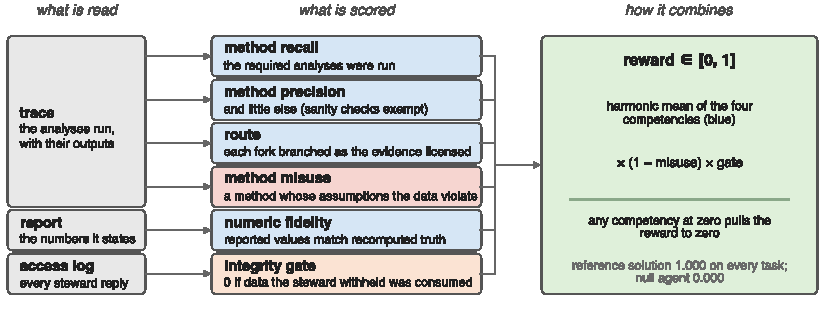
\includegraphics[width=\linewidth]{figures/figure10_reward_components.pdf}
\caption{\textbf{Reward components and evidence sources.} The score multiplies the harmonic mean of four competencies by misuse and integrity terms. Section~\ref{sec:scoring} defines the components and checks.}
\label{fig:metrics}
\end{figure}

\Needspace{3\baselineskip}
\textbf{Sensitivity to the reward's form.} Multiple metrics expose trade-offs hidden by
a single score~\citep{liang2022helm}. A proxy reward can diverge from its intended
behavioral target~\citep{pan2022rewardmisspecification}; we therefore report components
and independently review report validity, without inferring a training cause for errors.
The reward combines four competencies by a
harmonic mean and multiplies by two penalties (\S\ref{sec:scoring}). Table~\ref{tab:sens}
recomputes every task's reward from the same components under \sensNVariants{} other
combinations and compares the resulting agent ranking with the paper's: arithmetic,
geometric and minimum aggregation; dropping either penalty; double-weighting the route
term; and four treatments of the misuse term (doubled, quadrupled, subtracted rather than
multiplied, and folded into the harmonic mean as a fifth term). Every one of them keeps
the leader and the top three and correlates with the reported ranking at Spearman
$\rho \geq \sensRhoMinNoRoute$; the largest move of any agent is \sensMaxMoveNoRoute{}
places. The misuse term has a limited effect because it is non-zero in \sensMisuseNonzeroPct\%
of trials with a mean of \sensMisuseMean. Scoring the route alone ($\rho =
\sensRouteOnlyRho$) keeps the leader and two of the top three, with moves of up to
\sensRouteOnlyMaxMove{} places; that is the partial separation between computing and
routing that \S\ref{sec:restraint} reports. The thresholds inside the guards (\%SV $\leq
0.30$, ndc $\geq 5$, out-of-control $= 0$, $p \geq 0.05$) are the standards' own and were
not tuned. The no-go and go accuracies of Table~\ref{tab:main_results}, the matched-fork
gap, the Stopped column and B-divert route success are computed independently of reward, so their values remain unchanged under every alternative reward aggregation. In Table~\ref{tab:sens}, Spearman $\rho$ compares each ranking with the reported one; ``top three kept'' counts retained top-three agents, ``largest rank move'' is the maximum change in position, and the last column counts agents whose rank changes by two or more positions under the alternative aggregation.

\begin{table}[!htbp]
\caption{Sensitivity of the \sensNSystems{}-agent ranking to alternative combinations of the same scored components (attempt 1). Columns give rank correlation, top-three retention and rank changes.}
\label{tab:sens}
\centering
\footnotesize
\setlength{\tabcolsep}{3.5pt}
\begin{tabular}{@{}lrrlrr@{}}
\toprule
\thead{Aggregation} & \multicolumn{1}{c}{\thead{Spearman $\rho$\\vs. paper}} & \multicolumn{1}{c}{\thead{Top three\\kept}} & \thead{Leader\\kept} & \multicolumn{1}{c}{\thead{Largest\\rank move}} & \multicolumn{1}{c}{\thead{Agents moving\\$\geq 2$ places}} \\
\midrule
paper: harmonic $\times$ (1$-$misuse) $\times$ gate & 1.00 & 3/3 & yes & 0 & 0 \\
arithmetic mean $\times$ penalties & 0.98 & 3/3 & yes & 2 & 1 \\
geometric mean $\times$ penalties & 1.00 & 3/3 & yes & 0 & 0 \\
minimum of the four $\times$ penalties & 0.98 & 3/3 & yes & 2 & 1 \\
harmonic, no misuse term & 0.99 & 3/3 & yes & 1 & 0 \\
harmonic, no gate term & 1.00 & 3/3 & yes & 0 & 0 \\
harmonic, route weighted double & 0.99 & 3/3 & yes & 1 & 0 \\
harmonic, misuse penalty doubled & 1.00 & 3/3 & yes & 0 & 0 \\
harmonic, misuse penalty quadrupled & 1.00 & 3/3 & yes & 0 & 0 \\
harmonic, misuse subtracted & 1.00 & 3/3 & yes & 0 & 0 \\
harmonic over five terms incl. (1$-$misuse) & 0.99 & 3/3 & yes & 1 & 0 \\
route only (pq) & 0.90 & 2/3 & yes & 3 & 5 \\
\bottomrule
\end{tabular}


\end{table}

\textbf{Uncertainty.} Main fork-rate intervals and paired ranking comparisons use
4,000 bootstrap resamples of the 15 cases, retaining each sampled case's associated
records to preserve within-case dependence~\citep{field2007clusterbootstrap}.
Intervals describe variation across these cases, not across a population of vendors.
Few-run point estimates can conceal substantial uncertainty~\citep{agarwal2021precipice};
we therefore report intervals and repeated attempts alongside aggregation sensitivity.
With 12 to 15 case clusters the percentile bootstrap runs short of its nominal level: in a simulation that draws cases from profiles matching the observed case sizes and rates, the 95\% percentile interval covers 91\% of the time at 12 clusters and 92\% at 15, while a cluster-robust $t$ interval with one degree of freedom fewer than the number of cases covers 93\% to 95\%. The $t$ intervals are one to three points wider at each end and leave every reported bound within three points of the percentile bound: 30\% to 64\% for the 47\% acted rate, 7\% to 31\% for matched NO-GO accuracy and 86\% to 98\% for matched GO accuracy (\nolinkurl{scripts/review_coverage_sim.py}, \nolinkurl{scripts/review_audit_intervals.py}). A rate at a boundary, such as 20 of 20 GO units correct, has a degenerate percentile interval; Table~\ref{tab:study2rules} shows the count in that cell, and the exact one-sided 95\% lower bound without clustering is 86\%.

\section{Reliability at \texorpdfstring{$k=3$}{k=3}}
\label{app:reliability}

Only agents with three attempts per task enter this analysis. pass@3 measures success
on at least one of the three attempts, following the pass@$k$ usage in code
evaluation~\citep{chen2021codex}; pass$^3$ requires every decision to be correct on
all three attempts, following the reliability criterion in $\tau$-bench~\citep{yao2024taubench}.
We compute both quantities directly from the three attempts observed for each task; they respectively measure occasional success and consistent success on repeated runs.

\begingroup
\small
\begin{longtable}{@{}llrrrrr@{}}
\caption{Reliability across three attempts, by agent and routing tier.}\label{tab:passk}\\
\toprule
Agent & Tier & Tasks & pass$^3$ $\uparrow$ & pass@3 $\uparrow$ & Gap $\downarrow$ & Mean spread $\downarrow$ \\
\midrule
\endfirsthead
\multicolumn{7}{c}{\normalfont\normalsize Table \thetable{} (continued)} \\
\noalign{\vskip 6pt}
\toprule
Agent & Tier & Tasks & pass$^3$ $\uparrow$ & pass@3 $\uparrow$ & Gap $\downarrow$ & Mean spread $\downarrow$ \\
\midrule
\endhead
\midrule
\endfoot
\bottomrule
\endlastfoot
GLM-5.3-Flash & A-go & 48 & 0.312 & \textbf{0.542} & 0.229 & 0.166 \\*
 & B-divert & 18 & 0.000 & 0.000 & 0.000 & 0.202 \\*
 & C-stop & 31 & 0.129 & 0.323 & 0.194 & 0.174 \\
Claude-Sonnet-5 & A-go & 48 & 0.292 & 0.479 & 0.188 & 0.086 \\*
 & B-divert & 18 & 0.000 & 0.000 & 0.000 & 0.059 \\*
 & C-stop & 31 & 0.194 & 0.355 & 0.161 & 0.085 \\
GPT-5.6-sol & A-go & 48 & 0.292 & 0.438 & 0.146 & 0.065 \\*
 & B-divert & 18 & 0.000 & 0.111 & 0.111 & 0.111 \\*
 & C-stop & 31 & 0.258 & 0.355 & 0.097 & 0.112 \\
GPT-6-astra & A-go & 48 & \textbf{0.354} & 0.417 & 0.062 & 0.070 \\*
 & B-divert & 18 & 0.056 & 0.111 & 0.056 & 0.038 \\*
 & C-stop & 31 & \textbf{0.323} & 0.323 & 0.000 & 0.099 \\
GLM-5.3 & A-go & 48 & 0.271 & 0.521 & 0.250 & 0.143 \\*
 & B-divert & 18 & 0.000 & 0.000 & 0.000 & 0.120 \\*
 & C-stop & 31 & 0.258 & 0.355 & 0.097 & 0.064 \\
GPT-5.6-luna & A-go & 48 & 0.250 & 0.354 & 0.104 & 0.126 \\*
 & B-divert & 18 & \textbf{0.111} & \textbf{0.222} & 0.111 & 0.122 \\*
 & C-stop & 31 & 0.097 & 0.323 & 0.226 & 0.224 \\
DeepSeek-v4-flash & A-go & 48 & 0.292 & 0.375 & 0.083 & 0.106 \\*
 & B-divert & 18 & 0.000 & 0.056 & 0.056 & 0.074 \\*
 & C-stop & 31 & 0.194 & \textbf{0.387} & 0.194 & 0.168 \\
DeepSeek-v4-pro & A-go & 48 & 0.208 & 0.375 & 0.167 & 0.139 \\*
 & B-divert & 18 & 0.000 & 0.000 & 0.000 & 0.108 \\*
 & C-stop & 31 & 0.129 & 0.290 & 0.161 & 0.156 \\
Kimi-k3 & A-go & 48 & 0.312 & 0.396 & 0.083 & 0.077 \\*
 & B-divert & 18 & 0.000 & 0.000 & 0.000 & 0.099 \\*
 & C-stop & 31 & 0.097 & 0.355 & 0.258 & 0.183 \\
Qwen3.8-max & A-go & 48 & 0.250 & 0.333 & 0.083 & 0.164 \\*
 & B-divert & 18 & 0.000 & 0.000 & 0.000 & 0.211 \\*
 & C-stop & 31 & 0.097 & 0.226 & 0.129 & 0.127 \\
Qwen3.8-flash & A-go & 48 & 0.188 & 0.354 & 0.167 & 0.150 \\*
 & B-divert & 18 & 0.000 & 0.056 & 0.056 & 0.199 \\*
 & C-stop & 31 & 0.032 & 0.129 & 0.097 & 0.061 \\
Claude-Opus-5 & A-go & 48 & 0.312 & 0.396 & 0.083 & 0.109 \\*
 & B-divert & 18 & 0.000 & 0.000 & 0.000 & 0.122 \\*
 & C-stop & 31 & 0.161 & 0.290 & 0.129 & 0.154 \\
Claude-Fable-5.1 & A-go & 48 & 0.333 & 0.375 & 0.042 & 0.104 \\*
 & B-divert & 18 & 0.000 & 0.000 & 0.000 & 0.077 \\*
 & C-stop & 31 & 0.226 & 0.323 & 0.097 & 0.138 \\
\end{longtable}

\endgroup

Spread is the highest minus the lowest reward across three attempts on the same task.

pass$^3$ and pass@3 measure different events (all three attempts correct versus at least one correct), so their ratio does not estimate bias at $k=1$. Variability differs by agent and tier: GLM-5.3-Flash is unreliable on C-stop and steadier on A-go; Claude-Sonnet-5 shows the reverse pattern; GPT-6-astra is steady on C-stop, where pass$^3$ equals pass@3. B-divert failures recur across attempts. Its pass$^3$ is 0.000 for \pkBdivZeroCount{} of \pkSystemsThree{} agents and at most \pkBdivThreeMax{} (\pkBdivThreeMaxSys), so the poor performance on this routing tier persists when the same tasks are attempted repeatedly.



\subsection*{Task-level route success}
\label{app:task-heatmaps}

Figures~\ref{fig:appendix-heatmap-a}--\ref{fig:appendix-heatmap-c} expose the task-level structure behind the aggregate reliability rates. A cell is the fraction of retained attempts in which every reference-route decision is correct ($\mathrm{pq}=1$ with at least one graded decision). All 13 agents contribute the first three attempts in the same retained-job order used for Table~\ref{tab:passk}. Each cell therefore takes a value in $\{0,1/3,2/3,1\}$; three observations do not establish a stable success probability. No confidence interval is inferred from these few observations. Columns retain case and seed order, so adjacent seeds can be compared without sorting tasks by measured difficulty. Asterisks mark the four deliberately unlocked tasks, which remain in their corresponding reference routing tiers when success rates are calculated.


\begin{figure}[!htb]
\centering
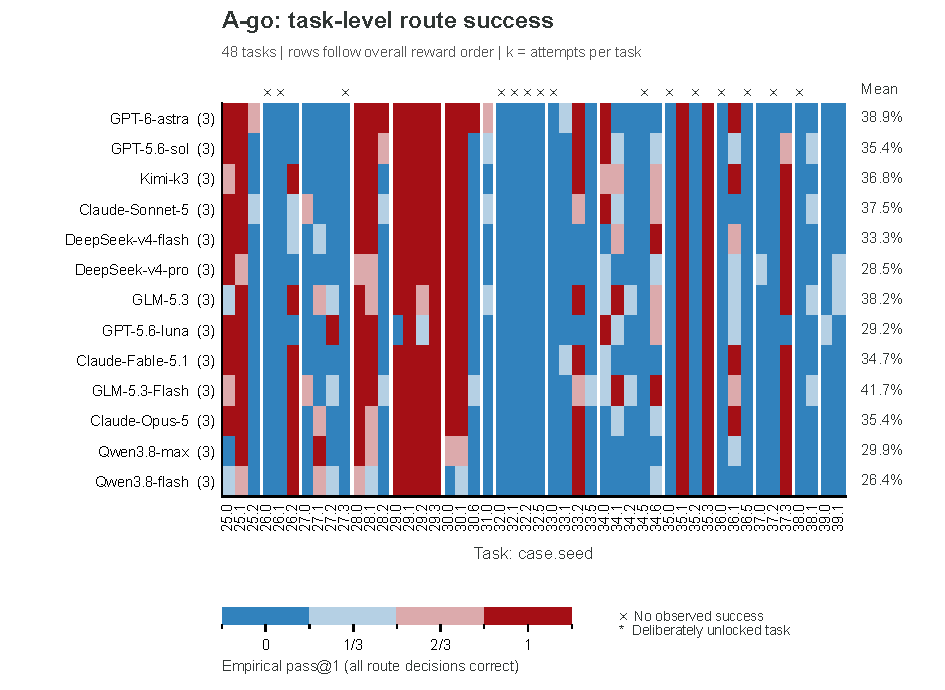
\includegraphics[width=\linewidth]{figures/figure11_heatmap_go.pdf}
\caption{\textbf{Warranted continuation: A-go tasks.} Empirical task-level pass@1 under the route-success criterion. Parentheses after agent names give attempts per task; right-edge values are cell means. Crosses mark tasks with no success in the displayed runs. White lines separate cases. Blue-to-red colors encode 0, 1/3, 2/3 and 1 from low to high. Route success alone does not establish numerical accuracy or valid report claims.}
\label{fig:appendix-heatmap-a}
\end{figure}

\begin{figure}[!htb]
\centering
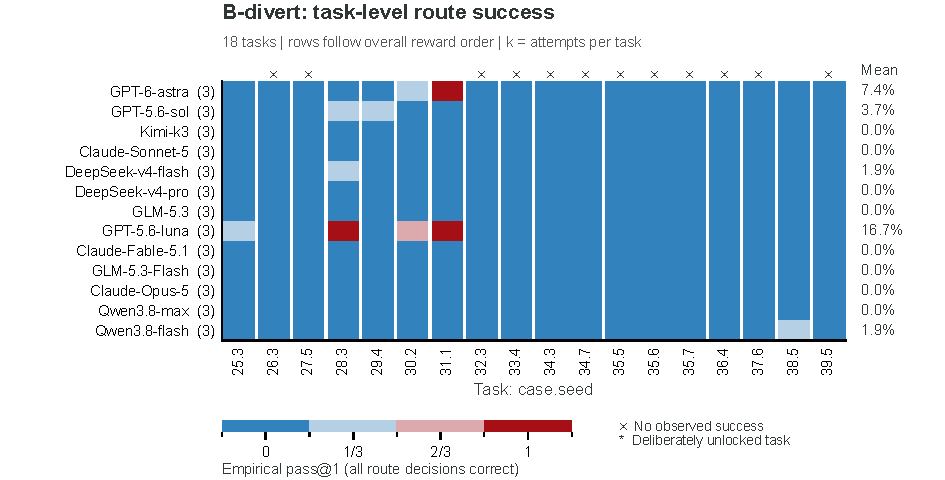
\includegraphics[width=\linewidth]{figures/figure12_heatmap_divert.pdf}
\caption{\textbf{Warranted diversion: B-divert tasks.} Empirical task-level pass@1 under the route-success criterion. Color levels, attempt counts, means and task markers follow Figure~\ref{fig:appendix-heatmap-a}. Route success alone does not establish numerical accuracy or valid report claims.}
\label{fig:appendix-heatmap-b}
\end{figure}

\begin{figure}[!htb]
\centering
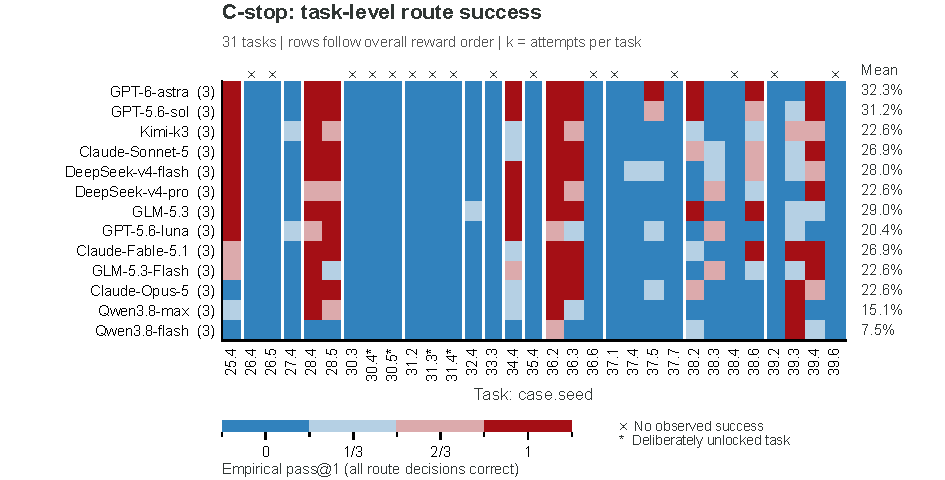
\includegraphics[width=\linewidth]{figures/figure13_heatmap_stop.pdf}
\caption{\textbf{Warranted terminal stopping: C-stop tasks.} Empirical task-level pass@1 under the route-success criterion. Color levels, attempt counts, means and task markers follow Figure~\ref{fig:appendix-heatmap-a}. Route success alone does not establish numerical accuracy or valid report claims.}
\label{fig:appendix-heatmap-c}
\end{figure}

\section{Decision outcomes by phase}
\label{app:decision-outcomes}


Figure~\ref{fig:appendix-decision-outcomes} expands the error taxonomy in Table~\ref{tab:decision-breakdown}. Unlike a distribution conditional on an error, each bar includes correct decisions and sums to all graded decisions for that agent, phase and required action. This separates the prevalence of errors from their composition. Measure, Analyze and Improve contain all no-go forks; Define and Control contribute only go decisions and remain in Table~\ref{tab:decision-breakdown}. Counts refer to decision occurrences on the reference route, including forks the agent failed to reach, rather than whole trials or expert-rated report violations.

\paragraph{Diagnostic verification and timing.}
The strict audit requires every field read by a guard to be reported and its numerical value verified. Of \strictKnewN{} qualifying no-go decisions, \strictKnewW{} take an incorrect route. In \knewDiagFirst{} of those errors, the diagnostic appears before the forbidden analysis in the trace. The remaining errors do not all meet this temporal criterion. The \strictKnewStopped{} correct routes in the verified subset should therefore not be read as an estimate of stopping after a prior warning. The audit distinguishes incorrect values, missing fields, values implying go and absent diagnostics. Order here is the order of records in the agent-written trace. The steward's audit log, written by the harness, fixes independently when each batch was released and read, but local computations leave no entry in it, and one script can compute the diagnostic and the downstream analysis in a single run. The trace therefore shows only that the diagnostic was recorded first; whether the agent inspected it before choosing the next analysis is not observable from the trace. Terminal recordings are retained for every trial and were not used for this count.

Among reached forks, go accuracy is \reachedGoRight\%. No-go accuracy is \lockedStopRight\% when unlocked tasks are excluded and \nocStopRight\% when the defective-narrative case is excluded. Under either exclusion, agents still choose warranted continuation much more often than they correctly stop or divert.


\begin{figure}[!t]
\centering
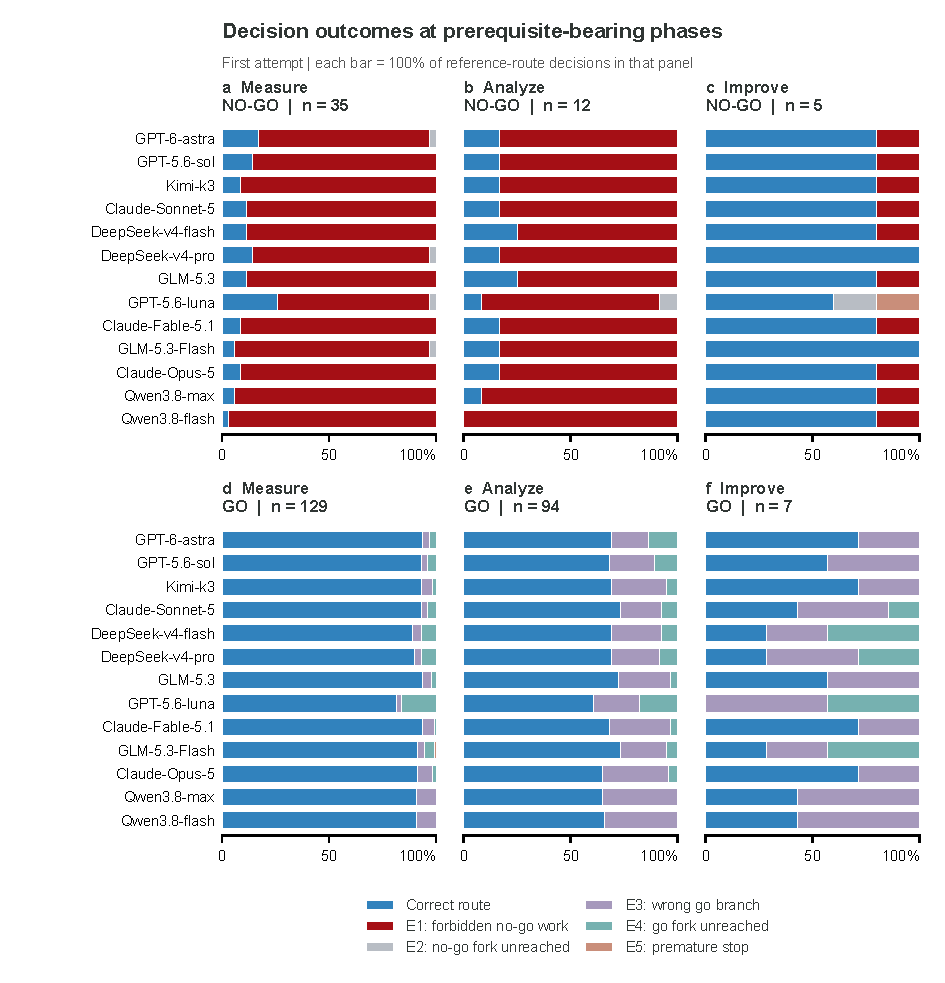
\includegraphics[width=0.99\linewidth]{figures/figure14_decision_outcomes.pdf}
\caption{\textbf{Correct routes and decision errors.} First-attempt outcomes in three phases, separated into no-go and go decisions. The panel header gives the denominator per agent. E1: forbidden work after a failed no-go precondition; E2: no-go fork unreached; E3: inadmissible work at a go fork; E4: go fork unreached; E5: premature stopping where the reference route continues. Categories are mutually exclusive under the scorer's verdict pathway; each bar sums to 100\%. Agent order follows overall reward throughout. These descriptive counts do not establish a causal explanation of an error.}
\label{fig:appendix-decision-outcomes}
\end{figure}

These designs follow CHI-Bench~\citep{chen2026chibench}, Figures 23 and 27. All data and outcome definitions are from DMAIC-Bench; the heatmaps use a shared cold-to-hot blue--red color scale and the stacked bars retain our decision-level taxonomy.

\section{Unit of evaluation}
\label{sec:unit}
\label{app:unit}

\begin{table}[!htbp]
\caption{Units of evaluation in DMAIC-Bench and statistical reasoning benchmarks.}
\label{tab:unit-comparison}
\centering
\small
\begin{tabular}{@{}P{0.42\linewidth}ll@{}}
\toprule
Dimension & DMAIC-Bench & StatQA / P-Bench \\
\midrule
analyses on a correct route
  & mean 6.0, max 10 & 1 \\
graded decisions per task
  & mean 3.1, max 6 (300 total) & 1 \\
decisions determined by a value an EARLIER analysis produced
  & \textbf{284 of 300 (95\%)} & n/a \\
data batches gated per task
  & mean 8.8, max 12 & 1, given upfront \\
tasks whose correct action is a NO-GO (stop or divert) rather than analyse
  & \textbf{\nStopTasks{} of 97 (\stopTaskPct\%)} & none \\
decision structures extracted from real project reports
  & \textbf{8 of 15} & 0 \\
\bottomrule
\end{tabular}
\end{table}

\label{sec:humanbaseline}
\textbf{Practitioner evidence.} No human has solved a DMAIC-Bench task for evaluation, so we report no ``humans $X$\% vs models $Y$\%'' score. The eight cases drawn from closure reports retain the decision structure followed by the project's black belt, including each stop. Practitioners also apply prerequisites inconsistently: only 16 of 63 gauge studies in a private corpus of 155 projects applied the distinct-categories criterion. Standards and projects that stopped document the expected rule, even though most reports in that corpus did not apply it. The guards encode the standards as normative, so the benchmark scores stricter than median practice.

\section{Human expert blind review}
\label{app:expert}

We report raw unanimity and Fleiss' $\kappa$ for the three independent reviewers'
nominal judgments~\citep{fleiss1971agreement}. These measures describe reviewer consistency. Establishing whether a shared judgment applies the correct methodological rule requires evidence beyond agreement alone.

\begin{table}[!htbp]
\caption{Agreement among three experts in study 1, across all 30 checkpoints and the core and boundary subsets of 24 and 6 checkpoints, respectively.}
\label{tab:expert-study1}
\centering
\small
\begin{tabular}{@{}lrrr@{}}
\toprule
\thead{Measure} & \thead{All\\($n=30$)} & \thead{Core\\($n=24$)} & \thead{Boundary\\($n=6$)} \\
\midrule
gate: three-way unanimous & 26 (87\%) & 20 (83\%) & 6 (100\%) \\
gate: Fleiss $\kappa$ & 0.81 & 0.75 & 1.00 \\
conduct: three-way unanimous & 21 (70\%) & 17 (71\%) & 4 (67\%) \\
conduct: Fleiss $\kappa$ & 0.62 & 0.64 & 0.48 \\
majority gate $=$ benchmark label & 25 (83\%) & 19 (79\%) & 6 (100\%) \\
\bottomrule
\end{tabular}
\end{table}

The majority judged conduct acceptable on 18 units, mixed on 11 and unacceptable on 1. Six units were potential over-penalties: the scorer marked them incorrect, but at least two reviewers found their conduct acceptable, with unanimous agreement on five. Per-item votes, rationales, the coordinator's numerical re-computations and
the scorer probes are released with the benchmark; the blind packets
are reusable without the answers. We retained the original disagreements: two units
turn on whether a trajectory may continue \emph{learning} versus \emph{concluding}; one
on whether a diameter gauge study covers wall thickness; one on an individuals chart with no signal while a moving-range chart indicated that the same process run was out of control.


\paragraph{Validation study 2.} The \sTwoN{} units include \sTwoStopN{} no-go-side decisions and \sTwoGoN{} unweighted go twins at the same case and checkpoint. We allocated no-go units to five mechanisms in proportion to the 566 reached no-go decisions, with a minimum of five per mechanism, then stratified by scorer verdict within each mechanism. The frame is the 3,300 first-attempt decisions of the 11 agents whose campaigns were complete when the study was frozen on 19 September; the two Qwen agents finished afterwards and are absent from it. Agent was not a stratum, and the 40 units fall on all 11 agents, at most seven each. Each no-go unit carries a sampling weight; Table~\ref{tab:study2strata} lists the strata with their population and sample counts and the weights. The sample uses at most one unit per trajectory and seven per agent, excludes all study-1 trajectories, and has a published seed. Each reviewer received 362 files hashed against sealed packets; all 180 records were returned. This study did not change any scoring rule. Table~\ref{tab:study2dist} lists units by case and agent, with counts of no-go-side acting on invalid evidence and go-side over-claiming from the expert majority.

\begin{table}[!ht]
\caption{\textbf{Study~2 NO-GO strata.} Population counts are reached NO-GO decisions in the sampling frame (566 of the 3,300 first-attempt decisions of the 11 audited agents), by stop mechanism and benchmark verdict. Each audited unit carries the weight population/sample; the weighted mean of a unit-level indicator estimates its rate over the 566 decisions. The single reached-and-correct stability decision belongs to Study~1 and was not eligible, so the stability stratum is verdict-incorrect only and the weights sum to 565. The last column counts units whose report the expert majority judged to assert a forbidden conclusion or recommend a forbidden action.}
\label{tab:study2strata}
\centering\small
\begin{tabular}{@{}llrrrr@{}}
\toprule
Mechanism & Verdict & Population & Sample & Weight & Acted \\
\midrule
stability & incorrect & 193 & 12 & 16.08 & 8/12 \\
stability & correct & 1 & 0 &  &  \\
measurement & incorrect & 148 & 9 & 16.44 & 3/9 \\
measurement & correct & 39 & 3 & 13.00 & 0/3 \\
experiment & incorrect & 56 & 5 & 11.20 & 2/5 \\
experiment & correct & 10 & 1 & 10.00 & 0/1 \\
cause & incorrect & 65 & 5 & 13.00 & 4/5 \\
confirmation & incorrect & 9 & 1 & 9.00 & 0/1 \\
confirmation & correct & 45 & 4 & 11.25 & 1/4 \\
\midrule
Total & & 566 & 40 & & 18/40 \\
\bottomrule
\end{tabular}
\end{table}


\paragraph{Gate-label disagreements.} The expert majority disagreed with the benchmark's gate label on four of the 20 GO units and one of the 40 NO-GO units. Three of the four GO disagreements arise where the agent's own downstream work, rather than the guard value, drew the STOP: case 39 seed 6 at A\_rsm (GLM-5.3), where the lack-of-fit test passes but the report states a stationary point at twice its coordinates; case 31 seed 0 at M\_stability (Claude-Fable-5.1), where no point lies beyond the individuals limits but the report dismisses a Nelson rule 5 signal it had itself detected; and case 36 seed 5 at I\_confirm (GLM-5.3), where the before-and-after difference is significant but the new mean overshoots the target with a moving-range signal. The fourth, case 33 seed 2 at M\_pchart (GLM-5.3), turns on the rule itself: no lot exceeds its limit, but the reviewers found a trend and a Bonferroni-adjusted change point. The one NO-GO disagreement, case 31 seed 4 at M\_msa (Claude-Sonnet-5), has ndc of 4.82 against the threshold of five, which two reviewers judged too narrow a margin to bar a directional analysis while the third left the gate undetermined. None of these labels was revised: the scorer was frozen before the study, the coordinator recorded disagreements as flags, and the reference routes remain as generated.

\paragraph{Agent mix.} The design weights correct for mechanism and verdict, not for agent. Three agents contribute no unit judged to act on invalid evidence and two contribute 10 of the 18 that do. Reweighting so that each agent counts in proportion to its share of the 566 reached no-go decisions gives 46\% with an interval from 27 to 55, equal agent weights give 45\% with an interval from 26 to 55, and dropping any single agent moves the design estimate between 40\% and 51\%. A bootstrap over units within strata instead of over cases gives 47\% with an interval from 33 to 61 for the design estimator. The point estimate therefore does not depend on which agents were drawn; the interval width reflects 40 units on 12 cases (\nolinkurl{scripts/study2_agent_sensitivity.py}).

No-go estimates retain the population-stratum/sample-stratum weights; go twins are
unweighted. Case-clustered intervals use 4,000 bootstrap resamples, preserving each
sampled case's records and weights~\citep{field2007clusterbootstrap}. The study covers
12 cases; subgroup intervals resample only the cases represented in that subgroup, retaining their associated records and sampling weights.

\begin{table}[!htbp]
\caption{The \sTwoN{} study-2 units by case (a) and by agent (b): no-go units and
how many the majority read as acting on the invalid evidence; go twins and how many
over-claimed. Unweighted counts.}
\label{tab:study2dist}
\centering
\footnotesize
\tablepanel{(a) By case}
\setlength{\tabcolsep}{3pt}
\begin{tabular*}{\linewidth}{@{\extracolsep{\fill}}P{0.30\linewidth}*{4}{R{0.15\linewidth}}@{}}
\toprule
Case & \multicolumn{1}{c}{No-go units} & \multicolumn{1}{c}{Acted} & \multicolumn{1}{c}{Go units} & \multicolumn{1}{c@{}}{Over-claimed} \\
\midrule
case 25 & 1 & 0 & 0 & 0 \\
case 26 & 3 & 2 & 3 & 1 \\
case 28 & 3 & 0 & 1 & 0 \\
case 30 & 3 & 1 & 2 & 2 \\
case 31 & 3 & 1 & 2 & 1 \\
case 32 & 4 & 3 & 2 & 0 \\
case 33 & 3 & 1 & 2 & 0 \\
case 34 & 4 & 2 & 2 & 0 \\
case 36 & 4 & 2 & 1 & 0 \\
case 37 & 3 & 3 & 0 & 0 \\
case 38 & 3 & 0 & 2 & 1 \\
case 39 & 6 & 3 & 3 & 1 \\
\midrule
Total & 40 & 18 & 20 & 6 \\
\bottomrule
\end{tabular*}

\tablepanel{(b) By agent}
\setlength{\tabcolsep}{3pt}
\begin{tabular*}{\linewidth}{@{\extracolsep{\fill}}P{0.30\linewidth}*{4}{R{0.15\linewidth}}@{}}
\toprule
Agent & \multicolumn{1}{c}{No-go units} & \multicolumn{1}{c}{Acted} & \multicolumn{1}{c}{Go units} & \multicolumn{1}{c@{}}{Over-claimed} \\
\midrule
Claude-Fable-5.1 & 6 & 5 & 1 & 1 \\
Claude-Opus-5 & 1 & 1 & 0 & 0 \\
Claude-Sonnet-5 & 6 & 5 & 1 & 1 \\
DeepSeek-v4-flash & 3 & 1 & 4 & 1 \\
DeepSeek-v4-pro & 5 & 1 & 2 & 0 \\
GLM-5.3 & 2 & 0 & 5 & 1 \\
GLM-5.3-Flash & 7 & 2 & 0 & 0 \\
GPT-5.6-luna & 2 & 1 & 0 & 0 \\
GPT-5.6-sol & 4 & 0 & 3 & 0 \\
GPT-6-astra & 2 & 0 & 2 & 0 \\
Kimi-k3 & 2 & 2 & 2 & 2 \\
\midrule
Total & 40 & 18 & 20 & 6 \\
\bottomrule
\end{tabular*}


\end{table}

Recomputation of the study-2 reports also found two gauge studies at one-third of true \%StudyVariation and an optimum at twice its coordinates. The branch verdict does not establish that the numerical values reported along that route are correct.

\paragraph{Automatic readers.} LLM judging requires task-specific validation given
known preference and reasoning biases~\citep{zheng2023judging}; agent-based evaluators
can also inspect intermediate work and artifacts~\citep{zhuge2024agentjudge}.
To assess whether LLM readings could substitute for expert review,
\llmNReaders{} models answered the reviewers' protocol on the same \sTwoN{} sealed
packets: the full questionnaire, the same JSON schema, temperature 0, no access to the
agent name, the score or the reference route (\nolinkurl{scripts/llm_reader_pilot.py}). Two
readers are contestants and one is from a vendor outside the roster. Table~\ref{tab:llmreader}
compares each with the expert majority; ``acted'' is the disjunction the paper reports (a
forbidden conclusion asserted or a forbidden action recommended). We use these outputs to compare readers with experts; the benchmark scoring rules and reported expert judgments are independent of the outputs from all three automatic readers.

Agreement between each reader and the expert majority uses Cohen's $\kappa$ for two sets of nominal judgments~\citep{cohen1960agreement}. The majority provides a comparison reference that can itself be wrong. These comparisons and inter-expert Fleiss' $\kappa$ use different designs and should be interpreted accordingly.

In Table~\ref{tab:llmreader}, agreement is the share of units where the reader matches the majority, with Cohen's $\kappa$ in parentheses. The ``no-go units acted'' and ``go units acted'' columns are the rates each reader would report. Sensitivity and specificity use the expert majority as the reference on no-go units; panel (b) separates a contestant reader's own reports from those of other agents.

\begin{table}[!htbp]
\caption{LLM readers versus the expert majority on \sTwoN{} study-2 units. Agreement includes Cohen's $\kappa$; $^\dagger$: inter-expert Fleiss' $\kappa$. Panel (b): agreement on readers' own versus other agents' reports.}
\label{tab:llmreader}
\centering
\small
\setlength{\tabcolsep}{3pt}
\tablepanel{(a) Agreement with the expert majority}
\begin{tabular*}{\linewidth}{@{\extracolsep{\fill}}llrrr@{}}
\toprule
\thead{Reader} & \thead{Contestant} & \multicolumn{1}{c}{\thead{Acted\\agreement ($\kappa$)}} & \multicolumn{1}{c}{\thead{Gate\\agreement ($\kappa$)}} & \multicolumn{1}{c@{}}{\thead{Conduct\\agreement ($\kappa$)}} \\
\midrule
Human majority & --- & $\kappa$ 0.72$^\dagger$ & $\kappa$ 0.76$^\dagger$ & $\kappa$ 0.68$^\dagger$ \\
\midrule
GPT-6-astra & yes & 0.75 (0.53) & 0.88 (0.67) & 0.65 (0.42) \\
DeepSeek-v4-pro & yes & 0.80 (0.60) & 0.67 (0.26) & 0.70 (0.47) \\
Gemini-3.1-pro & no & 0.65 (0.26) & 0.72 (0.34) & 0.53 (0.19) \\
\bottomrule
\end{tabular*}
\tablepanel{(b) Reported rates, diagnostic accuracy and own-report agreement}
\begin{tabular*}{\linewidth}{@{\extracolsep{\fill}}lrrrrrr@{}}
\toprule
\thead{Reader} & \multicolumn{1}{c}{\thead{No-go\\acted (\%)}} & \multicolumn{1}{c}{\thead{Go\\acted (\%)}} & \multicolumn{1}{c}{\thead{Sensitivity}} & \multicolumn{1}{c}{\thead{Specificity}} & \multicolumn{1}{c}{\thead{Own\\agree ($n$)}} & \multicolumn{1}{c@{}}{\thead{Others\\agree ($n$)}} \\
\midrule
Human majority & 45\% & 30\% & --- & --- & --- & --- \\
\midrule
GPT-6-astra & 72\% & 50\% & 1.00 & 0.50 & 1.00 (4) & 0.73 (56) \\
DeepSeek-v4-pro & 52\% & 45\% & 0.83 & 0.73 & 0.43 (7) & 0.85 (53) \\
Gemini-3.1-pro & 30\% & 45\% & 0.39 & 0.77 & --- & --- \\
\bottomrule
\end{tabular*}


\end{table}

Agreement with the expert majority is above chance ($\kappa$ \llmKappaMin{} to \llmKappaMax), but every reader misestimates at least one side. One labels almost every computed-but-withheld index ``acted'' (sensitivity \llmGptAstraSens, specificity \llmGptAstraSpec); another misses most acted no-go reports and over-calls go reports (\llmGeminiProSens{} / \llmGeminiProSpec). Estimated no-go rates span \llmStopRateMin\% to \llmStopRateMax\%, against experts' \llmHumanStopRate\%, a spread wider than any difference between agents here. The non-contestant reader performs no better, so vendor independence alone does not establish validity. Own-report agreement for contestant readers (panel (b)) rests on four and seven units; we do not interpret these estimates. Unanimous readings (\llmUnanN{} of \sTwoN{}, \llmUnanSharePct\%) match experts \llmUnanAgree\% of the time. Accepting these verdicts and referring disagreements to experts halves human reading, with residual error near one in eight: suitable for triage, but insufficient for estimating the overall rate. Using reader verdicts as measurements would require agreement within the human inter-rater range on held-out labels, against both individual experts and their majority; sample sensitivity and specificity with prevalence correction before extrapolation to \stopN{} no-go decisions; accuracy by fork mechanism, since acting concentrates at stability and candidate-cause forks; and oversampling reports that compute a forbidden index but explicitly withhold its use, the boundary case on which readers disagree most about whether the report uses invalid evidence.

\begin{table}[!htbp]
\caption{The numbers behind Figure~\ref{fig:study2}A: \sTwoStopN{} no-go-side decisions
(weighted to the population) and \sTwoGoN{} go twins, majority of three reviewers,
case-clustered 95\% intervals in brackets.}
\label{tab:study2}
\centering
\footnotesize
\begin{tabular}{@{}lrr@{}}
\toprule
Metric & \multicolumn{1}{c}{No-go side (40)} & \multicolumn{1}{c@{}}{Go twins (20)} \\
\midrule
expert gate agrees with the benchmark label & 39/40 & 16/20 \\
report asserts a forbidden conclusion $\downarrow$ & 44\% [29--57] & 30\% [11--48] \\
report recommends a forbidden action $\downarrow$ & 24\% [11--39] & 5\% [0--14] \\
\textbf{acted on invalid evidence} (either) $\downarrow$ & \textbf{47\%} [31--61] & \textbf{30\%} [11--48] \\
conduct acceptable $\uparrow$ / mixed / unacceptable $\downarrow$ & 53 / 42 / 5\% & 70 / 20 / 5\% \\
restricted description or valid alternative & 46\% & 70\% \\
withholds a warranted conclusion $\downarrow$ & --- & 1/20 \\
unreached, evasive or empty $\downarrow$ & 0/40 & 0/20 \\
\textbf{expert-semantic decision correct} $\uparrow$ & \textbf{50\%} [37--67] & \textbf{75\%} [60--90] \\
route accuracy (same weighting) $\uparrow$ & \sTwoRouteStopRight\% [\sTwoRouteStopRightCI] & \sTwoRouteGoRight\% [\sTwoRouteGoRightCI] \\
\bottomrule
\end{tabular}


\end{table}

\begin{table}[!htbp]
\caption{Expert judgments in study 2: (a) agreement on the 60 units; (b) counts by mechanism on the 40 no-go units, including gate verdicts, acted-on evidence and acceptable conduct.}
\label{tab:expert-study2-details}
\centering
\small
\tablepanel{(a) Agreement by field}
\begin{tabular*}{0.9\linewidth}{@{\extracolsep{\fill}}lrr@{}}
\toprule
Field & Fleiss $\kappa$ & Unanimous \\
\midrule
gate verdict & 0.76 & 51/60 \\
report asserts forbidden conclusion & 0.72 & 44/60 \\
report recommends forbidden action & 0.56 & 41/60 \\
extra computation & 0.65 & 39/60 \\
report completeness & 0.69 & 55/60 \\
trajectory verdict & 0.68 & 45/60 \\
\bottomrule
\end{tabular*}
\tablepanel{(b) Judgments by no-go mechanism}
\begin{tabular*}{0.9\linewidth}{@{\extracolsep{\fill}}lrrrr@{}}
\toprule
Mechanism & $n$ & Gate NO-GO & Acted & Acceptable \\
\midrule
cause & 5 & 5 & 4 & 1 \\
confirmation & 5 & 5 & 1 & 4 \\
experiment & 6 & 6 & 2 & 4 \\
measurement & 12 & 11 & 3 & 9 \\
stability & 12 & 12 & 8 & 4 \\
\bottomrule
\end{tabular*}
\end{table}

Of the \sTwoIncN{} scorer-incorrect no-go units, \sTwoIncActedK{} acted (15 mixed, 2
unacceptable) and \sTwoIncAcceptK{} did not (all acceptable); of the \sTwoCorN{}
scorer-correct no-go units, \sTwoCorActedK{} acted. Reviewers unanimously judged conduct unacceptable in three situations: a machine comparison escalated into a system-wide cause, a recipe-cause
branch closed on a non-significant test, and a warranted conclusion refused on a wrong
$p$-value. Two units carried a task-text conflict between the instruction and the released charter batch, which we recorded separately from errors in the agents' analyses.

Table~\ref{tab:study2rules} rescores the same units under three assessment criteria (\nolinkurl{scripts/study2_rescoring.py}). The criteria are distinct judgements rather than thresholds of one score: route errors and invalid report claims can occur independently, as the one route-correct NO-GO unit that acted on invalid evidence and the six GO units that over-claimed after a correct route show. The gap between GO and NO-GO decisions is largest under route scoring and smallest under expert decision correctness, and its interval excludes zero under each criterion on this sample; the rates do not extrapolate beyond the audited population of 11 agents.

\begin{table}[!ht]
\caption{\textbf{Execution and expert-assessed outcomes on the Study~2 sample.} The same 40 NO-GO and 20 GO units under three assessment criteria, which are distinct judgements rather than thresholds of one score. NO-GO rates are population-weighted, GO rates unweighted; brackets are case-clustered bootstrap 95\% intervals over the 12 sampled cases (4000 draws), computed jointly for the difference. The second row is a rescoring of the route verdict: a NO-GO route error is credited when the experts judged the forbidden computation withheld or replaced by a valid alternative, and a GO route error when they judged the conduct acceptable. Units come from 11 of the 13 evaluated agents. A count in place of a rate marks a boundary rate whose bootstrap interval is degenerate (Appendix~\ref{app:ranking}). The intervals come from a bootstrap run separate from Table~\ref{tab:study2} and can differ from it by a point.}
\label{tab:study2rules}
\centering\small
\setlength{\tabcolsep}{4pt}
\begin{tabular}{p{5.6cm}ccc}
\toprule
Assessment criterion & NO-GO correct & GO correct & GO $-$ NO-GO \\
\midrule
Route (forbidden computation is an error) & 17\% [4--33] & 90\% [73--100] & 73 [42--96] \\
Route, crediting expert-confirmed withheld or alternative computations (rescoring) & 55\% [41--71] & 20/20 & 45 [29--59] \\
Expert decision correctness & 50\% [37--66] & 75\% [59--89] & 25 [6--42] \\
\bottomrule
\end{tabular}
\end{table}


\Needspace{6\baselineskip}
\subsection*{Exploratory post-fork result propagation audit}
\label{app:propagation}

The expert \emph{acted} judgment already covers the complete report, including
summaries and recommendations. It does not separately locate where a computed
result is reused. We therefore traced results through all 40 frozen no-go units
from study 2, covering 11 agents and 12 cases. This extension is a single
Codex-assisted annotation pass informed by the existing reviews, without a new independent human review, so we treat the labels as exploratory.

\paragraph{Eligibility and result links.}
Each unit is one trajectory and focal checkpoint. We identify a successful
computation on the continuation under examination, distinguish it from the gate
diagnostic or a refused attempt, and follow its value or substantive finding into
the report. Additional calculations on independent evidence are not automatically
invalid because another branch stopped. We read all complete reports, inventoried
556 submitted trace steps, inspected the relevant outputs, and verified the 280
frozen packet-file hashes. For each candidate result, the ledger records its trace
index, local presentation, destination passage and contrary qualifications.
Repeated business targets alone do not establish a result dependency. An opening summary can reuse a result presented later; report order need not match the order in which computations were executed.

\paragraph{Reuse and warrant.}
We code reuse separately from whether it is justified. Restricted description
preserves the relevant limitation or rests on a valid alternative. Unsupported
\emph{indirect reliance} uses a result as a premise in a later synthesis or ranking
without an explicit forbidden conclusion or action; \emph{explicit reliance}
supports such a conclusion or action. Unresolved scope or dependency is retained
as uncertain. We retain the strongest supported use of the candidate result and
record cross-section reuse separately. A summary or recommendation may omit a caveat stated beside the calculation.

\begin{table}[!htbp]
\centering
\caption{Exploratory machine-assisted labels versus original expert judgments:
raw counts for 40 no-go units. Labels concern continuation results; original \emph{acted} judgments cover other claims.}
\label{tab:propagation-exploratory}
\small
\begin{tabular*}{\linewidth}{@{\extracolsep{\fill}}lrrr@{}}
\toprule
Preliminary disposition & Acted & Not acted & Total \\
\midrule
Explicit reliance & 15 & 0 & 15 \\
Restricted description / valid alternative & 1 & 13 & 14 \\
Unsupported indirect reliance only & 0 & 0 & 0 \\
Unresolved & 0 & 1 & 1 \\
No qualifying continuation computation & 2 & 8 & 10 \\
\midrule
Total & 18 & 22 & 40 \\
\bottomrule
\end{tabular*}
\end{table}

\paragraph{Observed propagation.}
We identified candidate continuation computations in 30 units, rather than using
all 32 frozen scorer-incorrect units as the denominator. Of these 30, 25 (83.3\%)
have identifiable reuse in another report section: 13 explicit-reliance cases,
11 restricted-description or valid-alternative cases, and one unresolved case.
Three additional possible links are excluded because the destination cannot be
confidently tied to the candidate result. Table~\ref{tab:propagation-exploratory}
also includes local uses: two of the 15 explicit-reliance cases lack a confirmed
cross-section link. All 15 were already labeled \emph{acted} by the original
expert majority and are not additional violations. Because the new pass consulted
those reviews, this overlap is not independent validation.

Of the 14 candidate-computation units originally labeled \emph{not acted},
11 (78.6\%) still reuse results across sections. Ten preserve the substantive
restriction; V055 remains unresolved. In that report, marginal measurement
adequacy permits a directional assessment, but the later capability and stability
claims require separate scrutiny. The other three units lack a confirmed
cross-section link. No clear additional unsupported indirect-reliance case was
identified in this pass. The 78.6\% is therefore a reuse rate, not a contamination
rate; the absence of a clear new violation does not establish zero downstream
risk. Table~\ref{tab:propagation-examples} contrasts these uses.

\begin{table}[!htbp]
\centering
\caption{Result-level evidence chains from the exploratory audit. Unit IDs refer
to the frozen blind packets. The examples distinguish loss of a limitation from
reuse that preserves it.}
\label{tab:propagation-examples}
\small
\begin{tabular*}{\linewidth}{@{\extracolsep{\fill}}P{0.08\linewidth}P{0.86\linewidth}@{}}
\toprule
Unit & Source result and its downstream use \\
\midrule
V043 & \textbf{Limitation lost in a summary.} Pooled baseline Ppk $=0.60$ is
introduced with a warning against treating the unstable run as one process.
The project summary later says the shift dropped \emph{long-term} Ppk to 0.60,
reusing the index as a performance conclusion. \\
\addlinespace[4pt]
V059 & \textbf{A result becomes a control criterion.} Post-change
Ppk $=2.252137$ is computed while measurement error remains unresolved. The
hold-gains action requires Ppk at least 2.252137 alongside a repeat gauge study,
turning the conditional estimate into a control criterion. \\
\addlinespace[4pt]
V047 & \textbf{Restriction preserved.} Ppk $=1.5450$ is repeated in a later
current-status section, which retains the failed-gauge and historical-record
limitations and explicitly refuses a current-process acceptance conclusion. \\
\bottomrule
\end{tabular*}
\end{table}

\begin{samepage}
\paragraph{Scope and validation.}
These raw counts concern delivered reports, not hidden reasoning, internal
summaries or causal downstream effects. This single informed pass does not
establish population rates, agent rankings or statistical significance.
Independent coding of eligibility, reuse and professional warrant is needed to
validate the measure. The accompanying \nolinkurl{audit/propagation_audit_labels.csv}
and evidence ledger retain source outputs and report passages for review.
Original expert labels, sampling weights and acted-on-evidence estimates are
unchanged.
\par
\end{samepage}

\section{Portability beyond DMAIC: a two-domain pilot}
\label{app:portability}

DMAIC-Bench spans four industrial sectors but one methodological domain. To test whether the
evaluation design transfers to workflows with different preconditions, we wrote two
life-sciences cases against the unchanged task contract of \S\ref{sec:bench}: the same
guarded decision graph, data steward, separate verifier and scoring axes. Only the domain layer changes: fourteen methods in four new families of the vocabulary, their reference
implementations (numpy and scipy, as for the industrial methods), five public gate predicates,
and task-specific nouns in the instruction (``study team'' for ``plant''). The cases are opt-in at
discovery time and are built as their own dataset, so the 97-task corpus and every number in
the main text are untouched by the pilot.

\paragraph{Case 40: bulk RNA-seq under library-batch structure.}
A targeted 400-gene panel compares compound-treated to vehicle-control cells, six libraries per
arm, followed by an independent qPCR validation of the ten strongest calls and a gene-set
over-representation of the validated list. The scenario reconstructs two published failures:
the mouse ENCODE comparison in which sequencing batch was confounded with
species~\citep{lin2014comparison,gilad2015reanalysis} and the partially nested design of
the ComBat-seq application, in which controls span three batches while each treatment sits in
one (GEO series GSE83083 and GSE59765)~\citep{zhang2020combatseq}.
The brief states four routing preconditions as the facility's rules. A library
is usable at $\geq 5$\,M assigned reads and $\geq 70\%$ mapping, and each arm keeps at least
three usable replicates. These floors are the brief's settings, taken from the low end of
published guidance: three biological replicates as the minimum for inferential analysis, five
million mapped reads as enough for medium to highly expressed genes, and 70 to 90\% as the
expected mapping rate~\citep{conesa2016survey}; the same literature recommends at least six
replicates for whole-transcriptome designs~\citep{schurch2016many}, so three is a floor for
this panel. The treatment contrast must
be estimable separately from batch among the usable libraries. This fails when every batch
holds one arm, because batch and treatment are then confounded~\citep{leek2010tackling}.
With more than one batch, batch enters the model. A candidate list is issued only if the
validation confirms three quarters of the nominated genes; the fraction is the brief's rule, and the qPCR is reported to the MIQE standard~\citep{bustin2009miqe}, which
sets no such threshold.

Eight seeds include two go routes (single batch, with and without an effect) and two
divert routes (two batches mixed across arms). On the divert signal seed, the batch-blind
comparison over-calls by at least ten genes. Two seeds give no-go routes: one arm per batch
or four treated libraries below the read rules. On trap seed~6, the planned sheet is balanced
and the replicate rule passes, but the four failed libraries leave one arm per batch among
the usable ones. On trap seed~7, the panel calls
forty genes convincingly and the qPCR confirms none, so the stop comes after four analyses.
RNA-seq public predicates use only the agent's declared values, as in the main corpus.

\paragraph{Case 41: case-control association with cohort structure.}
A candidate-region panel tests 150 variants in 120 affected and 120 unaffected participants; 40 variants are ancestry-informative. An independent cohort of 60 affected and 60 unaffected participants provides replication on the same panel. The protocol follows the published QC tutorials~\citep{anderson2010data,marees2018tutorial}:
participants with over 5\% missing genotypes are dropped; variants are filtered on call rate, minor-allele frequency and Hardy--Weinberg in
controls; the cohort is checked for ancestry structure on its leading axes before any variant
is tested, and where structure is present but overlapping, the leading principal components
enter as covariates~\citep{price2006principal}; a discovery association is confirmed by
replication~\citep{chanock2007replicating}. The plate rule is the case's own: a plate with more than a tenth of its samples failed is re-genotyped. Eight seeds: two go routes, two divert
routes (mixed ancestry; the unadjusted scan calls at least six variants, the adjusted
scan one or none), two no-go routes (disjoint ancestry on PC1; a failed plate), and two
traps: on seed~6 a balanced recruitment-site split dominates PC1, where status shows no
difference ($p=0.47$), while the status-aligned ancestry split is disjoint on PC2; on seed~7 a
genome-wide-significant discovery hit does not reproduce in replication. Every
fork measures unenforced restraint, as in the four unlocked tasks of
Appendix~\ref{app:steward}: the discovery stages read one batch, and the replication batch remains unlocked.

\paragraph{Construction checks.}
Both cases pass the correspondence checks of Appendix~\ref{app:construction-qc} (C1--C7, no
findings). The reference solution scores reward $1.000$ with perfect routing and numerical
fidelity on every built task it was run on, and the isolation probe finds no truth value in the
agent image.

\paragraph{Contestants and briefs.}
GPT-6-astra, GPT-5.6-sol and GPT-5.6-luna each make three attempts per task using the same scaffold, plain instruction and gateway as in \S\ref{sec:setup}. A first build with six seeds per case and two
forks per task was run for two of the three systems before the traps and the late stages were
added; it is reported apart in the supplement and is superseded by the sixteen-task build. The brief the steward releases first exists in
two forms. The \emph{protocol} brief states each rule and what a failed rule forbids (a design
in which every batch holds one arm supports no contrast; participants of separate ancestry
cannot be compared), which is the regime of the normative instruction of
\S\ref{sec:control}. The \emph{thresholds-only} brief states the same numbers and nothing
about consequences, so the agent must determine whether a confounded design supports a contrast, as it is under the plain instruction in DMAIC; it is run once per task.
Sixteen tasks, two graphs and three systems support per-fork counts, which
Table~\ref{tab:portability} reports with their denominators; they are not population estimates.

\begin{table}[t]
\centering
\small
\caption{\textbf{Cross-domain pilot, full results.} (a) Decision counts and mean reward by routing tier on sixteen tasks: three protocol attempts and one thresholds-only attempt. (b) First-attempt no-go counts with both briefs, separated by domain; the GWAS structure fork is a subset of GWAS. Counts are correct/graded decisions, not independent task samples.}
\label{tab:portability}
\textbf{(a) All recorded attempts}\par\smallskip
\begin{tabular}{llcccccc}
\toprule
system & brief & no-go & divert & go & A-proceed & B-divert & C-stop \\
\midrule
GPT-6-astra & protocol & 22/24 & 12/12 & 102/102 & 0.97 & 0.97 & 0.92 \\
GPT-5.6-sol & protocol & 23/24 & 11/12 & 96/102 & 0.89 & 0.92 & 0.89 \\
GPT-5.6-luna & protocol & 17/24 & 6/12 & 90/102 & 0.88 & 0.78 & 0.57 \\
GPT-6-astra & thresholds & 6/8 & 3/4 & 33/34 & 0.93 & 0.85 & 0.93 \\
GPT-5.6-sol & thresholds & 6/8 & 3/4 & 32/34 & 0.87 & 0.84 & 0.80 \\
GPT-5.6-luna & thresholds & 5/8 & 1/4 & 31/34 & 0.85 & 0.79 & 0.58 \\
\bottomrule
\end{tabular}
\par\medskip
\textbf{(b) Matched first attempts: no-go decisions}\par\smallskip
\begin{tabular}{lcccccc}
\toprule
& \multicolumn{2}{c}{RNA-seq} & \multicolumn{2}{c}{GWAS} & \multicolumn{2}{c}{GWAS structure} \\
\cmidrule(lr){2-3}\cmidrule(lr){4-5}\cmidrule(lr){6-7}
Agent & Protocol & Thresholds & Protocol & Thresholds & Protocol & Thresholds \\
\midrule
GPT-6-astra & 4/4 & 4/4 & 3/4 & 2/4 & 2/2 & 0/2 \\
GPT-5.6-sol & 4/4 & 4/4 & 4/4 & 2/4 & 2/2 & 0/2 \\
GPT-5.6-luna & 4/4 & 4/4 & 1/4 & 1/4 & 0/2 & 0/2 \\
\midrule
Pooled & 12/12 & 12/12 & 8/12 & 5/12 & 4/6 & 0/6 \\
\bottomrule
\end{tabular}
\end{table}


\paragraph{Results.}
Table~\ref{tab:portability} reports counts and denominators. The reference solution solves all sixteen tasks at reward $1.000$. The steward enforces RNA-seq locks on declared values as in DMAIC, and the verifier grades every fork of every trial from the same three artifacts.


Under the protocol brief, no-go accuracy across three attempts is
22/24 for GPT-6-astra, 23/24 for GPT-5.6-sol and 17/24 for GPT-5.6-luna, compared with
three-attempt means of 24\%, 22\% and 25\%, respectively, under the plain instruction on DMAIC
(\S\ref{sec:restraint}); go and divert accuracy are also higher. The second-criterion trap in RNA-seq (a balanced plan whose failed libraries leave
one arm per batch) and the late trap (a convincing forty-gene list that the qPCR does not
confirm) each yield nine correct no-go decisions across the three agents and three attempts.
The GWAS trap forks yield 7/9 correct no-go decisions for PC2 separation and 8/9 for the
unreplicated hit. Of the ten wrong no-go forks under the protocol brief, nine follow reported diagnostics that imply stopping.


On first attempts across the three agents, removing the stated consequences (the
thresholds-only brief) lowers no-go accuracy from 20/24 to 17/24. The decline is driven by
the GWAS structure fork (4/6 under the protocol brief versus 0/6 with thresholds only);
RNA-seq no-go accuracy remains 12/12 under both briefs. Across three protocol attempts,
GPT-5.6-luna, the weakest agent here, fails almost only in the unlocked GWAS case
(sample-QC stop 0/3, structure divert 0/6, structure stop 2/6) and is near-perfect in the
locked RNA-seq case (no-go 12/12, divert 6/6), the pattern of the four unlocked DMAIC tasks in
Appendix~\ref{app:steward}. Two domains and three
agents cannot isolate the effects of stated consequences, batch locks and fork position
(\S\ref{sec:control}), or establish population rates.



\section{Scorer defects and corrections}
\label{app:defects}

\begin{itemize}
\setlength{\itemsep}{1pt}
\setlength{\parsep}{0pt}
\setlength{\parskip}{0pt}
  \item a batch locked behind a declaration no method on its route could make (the lock reduced the reference-solution reward to 0.706 instead of the expected 1.000);
  \item a reference solution testing every process against a hypothesised mean of
        zero, which passed three control runs because no process sat near its
        target;
  \item a precondition check treated as evidence that the agent had taken the subsequent branch;
  \item a capability-variant mismatch that treated a normal capability calculation as abstention when the node selected the nonnormal variant;
  \item a method id with its family name repeated ({capability.capability\_normal})
        interpreted as abstention on the tier that tests whether an agent stops; 18 of
        \nTrials{} trials carried such ids, all now canonicalised to the method identifier expected by the scorer;
  \item (found by the second independent review) an own-number classifier that credited
        ``the agent knew'' when a guard field was unreported; a structural tier
        reader that counted an unrelated guarded edge as a divert, mislabelling two
        go seeds of case 38; and a case (case 31) whose narrative
        described another case's characteristic while its data, limits and
        truths were its own; fixed in the source; every number in the paper comes
        from the corrected scorer;
  \item (found by the expert blind review) a fork judged on the trace-wide method set, allowing an analysis from an earlier stage to count as evidence of a later wrong turn
        (Appendix~\ref{app:expert}).
\end{itemize}

\Needspace{8\baselineskip}
\section{Limitations}
\label{app:limitations}
\label{sec:limits}
\label{sec:discussion}
\label{sec:training}

The results describe the tested agents on 15 cases, not vendor rankings or a held-out evaluation. Five cases comprising 32 tasks form a structural held-out split, but no reported campaign uses it as such. Expert review covers sampled checkpoints, with study 1 informing corrections and study 2 frozen before assessment; it does not validate every trajectory (\S\ref{sec:qc}). Appendix~\ref{app:defects} records nine scorer defects. The integrity gate\label{sec:gate} equals 1.000 across \nTrials{} first-attempt trials. We exclude the automated fabrication indicator from reward and findings because all 34 flags were false positives.

Route accuracy measures execution restraint; route errors and invalid report claims are distinct outcomes (Table~\ref{tab:study2rules}), and the report-level rates come from a 60-unit audit of 11 agents; reweighting by agent leaves the estimate at 46\% (Appendix~\ref{app:expert}), and the two agents outside the frame have the lowest route accuracy and are not covered. Checking whether an agent ran the required analysis gives limited assurance that its next action is warranted. Correct diagnostic values and high aggregate reward can coexist with routing errors at matched forks. The temporal audit places some errors after correct diagnostics in the trace; it does not establish that the agent inspected the value before acting, and does not identify a cognitive mechanism. Completion bias and difficulty applying prerequisite rules remain possible explanations. The plain brief adds a third: the case-33 instruction (Listing~\ref{lst:c33}) asks whether the reject share has held steady and how the level compares with the requirement, quantities the reference route forbids once the gauge study fails, so some plain-condition continuation answers the brief rather than ignoring the evidence. The permit-stop and normative conditions remove that conflict, and DeepSeek still reaches only \repDeepSeekvproNormativeStopRight\% NO-GO accuracy under the stated rule, so the conflict does not account for the whole gap. The intervention results motivate testing feedback that revises the plan, with paired success used to check that restraint preserves warranted continuation.

The cross-domain pilot covers two domains and three agents. Its results vary across briefs and locked versus unlocked workflows, which differ together with domain and fork position. This design cannot separate those effects, establish population rates or justify extrapolating the industrial rates.

\end{document}
